%\documentclass[10pt,a5paper]{memoir}
\documentclass[11pt]{memoir}

\usepackage[margin=1in]{geometry}
%\usepackage[margin=0.75in]{geometry}
%\usepackage[protrusion=true,expansion=true]{microtype}

%\usepackage[center]{titlesec}

\usepackage[pdftex,
	    pdftitle={Algebraic topology}]{hyperref}
%\usepackage{spectralsequences}

\usepackage{mathtools}
%\usepackage{listings}

\usepackage[T1]{fontenc}

%\usepackage[urw-garamond]{mathdesign}
%\usepackage[left=2in,right=2in,top=2in,bottom=2.5in]{geometry}
%\usepackage[margin=1.25in]{geometry}
%\pagestyle{plain}
%\usepackage{fullpage}

\usepackage{setspace}
%\setstretch{1.1}

\usepackage{todonotes}

\usepackage{amsmath}
%\usepackage{amsfonts}
\usepackage{amssymb}
\usepackage{float}
\usepackage{amsthm}
\usepackage{comment}
%\usepackage{amscd}

%\usepackage{txfonts} % Thanks to Eric for showing me that this font exists.
%%\usepackage{kpfonts}
%\renewcommand{\Top}{\mathbf{Top}}
\newcommand{\Top}{\mathbf{Top}}

\usepackage{color}
\usepackage[all]{xy}
\usepackage{verbatim}

\usepackage[mathscr]{eucal}
\usepackage{graphicx}
\usepackage{tikz-cd}

\usepackage{chngcntr} % to number sections consecutively across chapters
\counterwithout{section}{chapter}

\tikzset{%
    symbol/.style={%
        draw=none,
        every to/.append style={%
            edge node={node [sloped, allow upside down, auto=false]{$#1$}}}
    }
}

\theoremstyle{theorem}
\newtheorem{theorem}{Theorem}[section]
\newtheorem{thm-defn}[theorem]{Theorem-Definition}
\newtheorem{prop}[theorem]{Proposition}
\newtheorem{lemma}[theorem]{Lemma}
\newtheorem{corollary}[theorem]{Corollary}

\theoremstyle{definition}
\newtheorem{problem}[theorem]{Problem}
\newtheorem{definition}[theorem]{Definition}
\newtheorem{notation}[theorem]{Notation}
\newtheorem{summary}[theorem]{Summary}
\newtheorem{note}[theorem]{Note}
\newtheorem{claim}[theorem]{Claim}
\newtheorem{exercise}[theorem]{Exercise}
\newtheorem{terminology}[theorem]{Terminology}
\newtheorem{construction}[theorem]{Construction}
%\theoremstyle{remark}
\newtheorem{remark}[theorem]{Remark}
\newtheorem{example}[theorem]{Example}
\newtheorem{question}[theorem]{Question}
\newtheorem{slogan}[theorem]{Slogan}
\newtheorem{warning}[theorem]{Warning}
\newtheorem{solution}[theorem]{Solution}
\newtheorem{property}[theorem]{Property}

\DeclareMathOperator{\Th}{Th}
\DeclareMathOperator{\Aut}{Aut}
\DeclareMathOperator{\coeq}{coeq}
\DeclareMathOperator{\colim}{colim}
\DeclareMathOperator{\coker}{coker}
\DeclareMathOperator{\cone}{cone}
\DeclareMathOperator{\Der}{Der}
\DeclareMathOperator{\Ext}{Ext}
\DeclareMathOperator{\Fun}{Fun}
\DeclareMathOperator{\hocolim}{hocolim}
\DeclareMathOperator{\holim}{holim}
\DeclareMathOperator{\Hom}{Hom}
\DeclareMathOperator{\Iso}{Iso}
\DeclareMathOperator{\img}{im}
\DeclareMathOperator{\Map}{Map}
\DeclareMathOperator{\Tot}{Tot}
\DeclareMathOperator{\Tor}{Tor}
\DeclareMathOperator{\Res}{Res}
\DeclareMathOperator{\Spec}{Spec}
\DeclareMathOperator{\rank}{Rank}
\DeclareMathOperator{\Vect}{Vect}

\def\llarrow{  \hspace{.05cm}\mbox{\,\put(0,-2){$\leftarrow$}\put(0,2){$\leftarrow$}\hspace{.45cm}}}
\def\rrarrow{  \hspace{.05cm}\mbox{\,\put(0,-2){$\rightarrow$}\put(0,2){$\rightarrow$}\hspace{.45cm}}}
\def\lllarrow{ \hspace{.05cm}\mbox{\,\put(0,-3){$\leftarrow$}\put(0,1){$\leftarrow$}\put(0,5){$\leftarrow$}\hspace{.45cm}}}
\def\rrrarrow{ \hspace{.05cm}\mbox{\,\put(0,-3){$\rightarrow$}\put(0,1){$\rightarrow$}\put(0,5){$\rightarrow$}\hspace{.45cm}}}

\def\cA{\mathcal A}\def\cB{\mathcal B}
\def\cc{\mathcal C}\def\cC{\mathbf C}
\def\cd{\mathcal D}
\def\ce{\mathcal E}\def\cf{\mathcal F}\def\cG{\mathcal G}\def\cH{\mathcal H}
\def\cI{\mathcal I}\def\cJ{\mathcal J}\def\cK{\mathcal K}\def\cL{\mathcal L}
\def\cM{\mathcal M}\def\cN{\mathcal N}\def\cO{\mathbf O}\def\cP{\mathcal P}
\def\cQ{\mathcal Q}\def\cR{\mathcal R}\def\cS{\mathcal S}\def\cT{\mathcal T}
\def\cU{\mathcal U}\def\cV{\mathcal V}\def\cW{\mathcal W}\def\cX{\mathcal X}
\def\cY{\mathcal Y}\def\cZ{\mathcal Z}

\def\AA{\mathbb A}\def\BB{\mathbb B}\def\CC{\mathbf C}\def\DD{\mathbb D}
\def\EE{\mathbb E}\def\FF{\mathbf F}\def\GG{\mathbb G}\def\HH{\mathbb H}
\def\II{\mathbb I}\def\JJ{\mathbb J}\def\KK{\mathbb K}\def\LL{\mathbb L}
\def\MM{\mathcal M}\def\NN{\mathbb N}\def\OO{\mathbb O}\def\PP{\mathbf P}
\def\QQ{\mathbf Q}\def\RR{\mathbf R}\def\SS{\mathbb S}\def\TT{\mathbb T}
\def\UU{\mathbb U}\def\VV{\mathbb V}\def\WW{\mathbb W}\def\XX{\mathbb X}
\def\YY{\mathbb Y}\def\ZZ{\mathbf Z}

\usepackage{amsbsy}

\newcommand{\CP}{\mathbf{CP}}
\newcommand{\RP}{\mathbf{RP}}
\newcommand{\Set}{\mathrm{Set}}
\newcommand{\Gra}{\mathrm{Gr}}
\newcommand{\GL}{\mathrm{GL}}
\newcommand{\gl}{\mathit{gl}}

\newcommand{\nn}{\nonumber}
\newcommand{\nid}{\noindent}
\newcommand{\ra}{\rightarrow}
\newcommand{\la}{\leftarrow}
\newcommand{\xra}{\xrightarrow}
\newcommand{\xla}{\xleftarrow}

\newcommand{\weq}{\xrightarrow{\sim}}
\newcommand{\cofib}{\rightarrowtail}
\newcommand{\fib}{\twoheadrightarrow}
%\newcommand{\cofib}{\to}
%\newcommand{\fib}{\to}

\newcommand\cHH{\check{H}}
\newcommand{\Fl}{\mathrm{Fl}}
\newcommand{\Fr}{\mathrm{Fr}}
\newcommand\cCC{\check{C}}
\newcommand{\MFGL}{\mathcal M_{\mathit{FGL}}}
\newcommand{\calO}{{\mathcal O}}
\newcommand{\calC}{{\mathcal C}}
\newcommand{\set}{{\mathrm{Set}}}
\newcommand{\Deltab}{{\Delta}} %change this to bold Delta. This is like this
%here because garamond messes up bold things.
\newcommand{\spec}{\mathrm{Spec}}
\newcommand{\Z}{\mathbf Z}
\newcommand{\Sin}{\mathrm{Sin}}
\newcommand{\htop}{\mathrm{Ho}(\mathbf{Top})}
\newcommand{\sca}{\mathcal{A}}
\DeclareMathOperator{\Spf}{Spf}
\newcommand{\CG}{\mathbf{CG}}
\newcommand{\Ab}{\mathbf{Ab}}
\newcommand{\Bun}{\mathrm{Bun}}
\newcommand{\Ho}{\mathrm{Ho}}
\newcommand{\gr}{\mathrm{gr}}
\newcommand{\sk}{\mathrm{sk}}
\newcommand{\Cat}{\mathbf{Cat}}
\newcommand{\wt}[1]{\widetilde{{#1}}}
\newcommand{\xar}[1]{\xrightarrow{{#1}}}
\newcommand{\pr}{\mathrm{pr}}
\newcommand{\ev}{\mathrm{ev}}
\newcommand{\inc}{\mathrm{in}}
\newcommand{\Spin}{\mathrm{Spin}}
\newcommand{\String}{\mathrm{String}}
\newcommand{\Sk}{\mathrm{Sk}}


\newcommand{\downsubseteq}{\mathbin{\rotatebox[origin=c]{-90}{$\subseteq$}}}

% for pullback and pushout squares
\usepackage{pigpen}
\newcommand{\po}{\ar@{}[dr]|{\text{\pigpenfont R}}}
\newcommand{\pb}{\ar@{}[dr]|{\text{\pigpenfont J}}}
%%%%%%%%%%%%%%%%

%\usepackage{ebgaramond}
%\usepackage{fancyhdr}
% 
%\newcommand{\myheader}{
%    \ifnum\value{section} > 38
%    18.906
%    \else
%    18.905
%    \fi
%}
%
%\pagestyle{fancy}
%\fancyhf{}
%\fancyhead[LE]{Notes by Sanath Devalapurkar}
%\fancyhead[LO]{Taught by Haynes Miller}
%\chead{Notes for \myheader}
%\rhead{Lecture \thesection}
%\cfoot{\thepage}

%\usepackage[urw-garamond]{mathdesign}



\begin{document}
\title{Algebraic Topology}
\author{Lectures by Haynes Miller\\
Notes based on live{\TeX}ed record made by Sanath Devalapurkar

}
%\date{Fall 2016 -- Spring 2017}

\frontmatter

\maketitle
\cleardoublepage
\section*{Preface}
Over the 2016--2017 academic year, I ran the graduate algebraic topology 
sequence at MIT. The first semester deals with singular homology and 
cohomology, and Poicar\'e duality; the second builds up basic homotopy theory,
spectral sequences, and characteristic classes. 

My goal was to give a standard classical approach to these subjects. 
In the first semester, I had various more specific objectives. 
I wanted to introduce students to the basic language of category theory
and simplicial sets, so useful throughout
mathematics and finding is first real manifestations in algebraic 
topology. I wanted to stress the methods of homological algebra,
for similar reasons. And I especially wanted 
to give an honest account of the machinery -- relative cap product and
\v{C}ech cohomology --  needed in the proof of Poincar\'e duality. 
The present document contains a bit more detail than was presented 
in the course.

On the other hand I barely touched on some important subjects. 
I did not talk about simplicial complexes at all.
I gave only a brief summary of
the theory of covering spaces and the fundamental group, in preparation
for a proper understanding of orientations. I avoided some point set
topology by working with only compact subspaces rather than general closed 
subspaces in the development of Poincar\'e duality.

I was lucky enough to have in the audience a student, Sanath Devalapurkar, 
who spontaneously decided to {live\TeX} the entire course. This resulted in 
a remarkably accurate record of what happened in the classroom -- right down
to random alarms ringing and embarassing jokes and mistakes on the blackboard. 
Sanath's \TeX forms the basis of these notes, and I am grateful to him 
for making them available. The attractive  drawings were provided by
another student, Xianglong Ni, who also carefully proofread the manuscript.

In the course of editing these notes, beyond correcting various errors 
(while hopefully not introducting new ones), I completed various arguments
not done in detail in the actual lectures, and rearranged some of the
material to take full advantage of hindsight. 




\newpage
%Here are hyperlinks to the notes from each of the semesters.
%    \begin{enumerate}
%        \item The notes for 18.905 start at section \ref{905}.
%        \item The notes for 18.906 start at section \ref{906}.
%    \end{enumerate}

%\section*{Stuff to fix}
%\begin{itemize}
%    \item The original version of the notes used
%	\verb|\cc| to denote both a script C and the complex numbers.
%	Now, \verb|\cc| denotes a script C and \verb|\cC| denotes the complex
%	numbers.
%	Everytime you find this, edit it!
%    \item Be consistent about your use of $\Hom_\cc(C,D)$ and $\cc(C,D)$ for hom-sets.
%\end{itemize}



%\section*{Things to fix}
%\begin{itemize}
%    \item As of \today, all of Part II has been edited, with the exception of
%	\S \ref{basepoints}, \S \ref{section-serre-classes}, \S
%	\ref{mod-c-hurewicz}, \S \ref{dress-sseq}, \S \ref{leray-hirsch}, and
%	\S \ref{gysin-sequence}.
%    \item Part I remains to be edited.
%    \item The original version of the notes used \verb|\cc| to denote both a
%	script C and the complex numbers.  Now, \verb|\cc| denotes a script C
%	and \verb|\cC| denotes the complex numbers. This is a problem that
%	needs to be fixed everywhere.
%\end{itemize}

\newpage
\tableofcontents
\newpage

\mainmatter

% The current division of labor is: John'll "work on the first part (like, most of 905)",
% and skd will start off by editing/rewriting the whole of 906.
%
%\part{18.905: an introduction to algebraic topology}\label{905}

\chapter{Singular homology}
% I removed the definition of a manifold and moved it in-line for better flow.
% I think it's best to use /emph in definitions to show what's being defined.
% Put periods even in display math!
% For spacing reasons, should use \colon instead of : for functions, e.g. f \colon A \to B.
% Since ker is lowercase, im probably should be also.

\section{Introduction: singular simplices and chains}\label{905}
This is a course on algebraic topology. 
We'll discuss the following topics. 
\begin{enumerate}
    \item Singular homology
    \item CW-complexes
    \item Basics of category theory
    \item Homological algebra
    \item The K\"{u}nneth theorem
    \item Cohomology
    \item Universal coefficient theorems
    \item Cup and cap products
    \item Poincar\'{e} duality.
\end{enumerate}
The objects of study are of course topological spaces, and the machinery
we develop in this course is designed to be applicable to a general space. 
But we are really mainly interested in geometrically important spaces. 
Here are some examples. 
\begin{itemize}
    \item The most basic example is \emph{$n$-dimensional Euclidean space}, $\mathbf{R}^n$.
    \item The \emph{$n$-sphere} $S^n=\{x\in \mathbf{R}^{n+1}:|x|=1\}$, topologized as a subspace of $\mathbf{R}^{n+1}$.
    \item Identifying antipodal points in $S^n$ gives \emph{real projective space} $\mathbf{RP}^n=S^n / (x\sim -x)$, i.e. the space of lines through the origin in $\mathbf{R}^{n+1}$.
    \item Call an ordered collection of $k$ orthonormal vectors an \emph{orthonormal $k$-frame}. The space of orthonormal $k$-frames in $\mathbf{R}^n$ forms the \emph{Stiefel manifold} $V_k(\mathbf{R}^n)$, topologized as a subspace of $(S^{n-1})^k$.
   \item The \emph{Grassmannian}  $\mathrm{Gr}_k(\mathbf{R}^n)$ is the space of
$k$-dimensional linear subspaces of $\mathbf{R}^n$. Forming the span gives us
a surjection $V_k(\mathbf{R}^n)\to\mathrm{Gr}_k(\mathbf{R}^n)$, and the
Grassmannian is given the quotient topology. 
For example, $\mathrm{Gr}_1(\mathbf{R}^n) = \mathbf{RP}^{n-1}$.
\end{itemize}
All these examples are \emph{manifolds}; that is, they are Hausdorff spaces locally homeomorphic to Euclidean space. Aside from $\mathbf{R}^n$ itself, the preceding examples are also compact. Such spaces exhibit a hidden symmetry, which is the culmination of 18.905: Poincar\'{e} duality.

As the name suggests, the central aim of algebraic topology is the usage of algebraic tools to study topological spaces. A common technique is to probe topological spaces via maps to them from simpler spaces. In different ways, this approach gives rise to singular homology and homotopy groups. We now detail the former; the latter takes the stage in 18.906.
\begin{definition}
For $n\geq 0$, the \emph{standard $n$-simplex} $\Delta^n$ is the convex hull of the standard basis $\{e_0,\ldots,e_n\}$ in $\mathbf{R}^{n+1}$:
$$\Delta^n = \left\{\sum t_i e_i : \sum t_i = 1, t_i\geq 0\right\}\subseteq\mathbf{R}^{n+1}.$$
The $t_i$ are called {\em barycentric coordinates}.
\end{definition}
%We will write $i$ in lieu of $e_i$ to refer to the vertices of $\Delta^n$. 
The standard simplices are related by face inclusions $d^i\colon \Delta^{n-1} \to \Delta^{n}$ for $0\leq i \leq n$, where $d^i$ is the affine map that sends
verticies to vertices, in order, and omits the vertex $e_i$.

\begin{center}
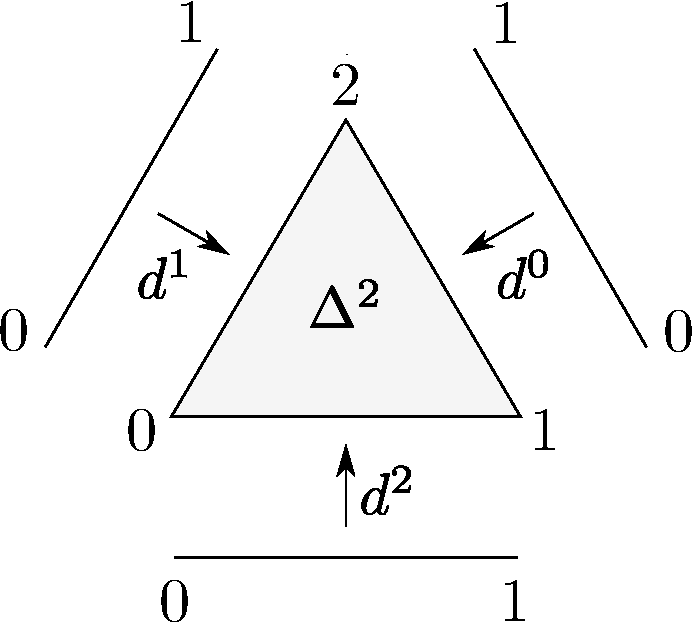
\includegraphics[width=2in]{905/Figures/01-2-simplex.pdf}
\end{center}

\begin{definition}
Let $X$ be any topological space. A \emph{singular $n$-simplex} in $X$ is a continuous map $\sigma:\Delta^n\to X$. Denote by $\mathrm{Sin}_n(X)$ the set of all $n$-simplices in $X$.
\end{definition}
    
This seems like a rather bold construction to make, as $\mathrm{Sin}_n(X)$ is huge. But be patient! 

For $0\leq i \leq n$, precomposition by the face inclusion $d^i$ produces a map $d_i\colon \Sin_n(X)\to\Sin_{n-1}(X)$ sending $\sigma\mapsto\sigma\circ d^i$. This is the ``$i$th face'' of $\sigma$. This allows us to make sense of the ``boundary'' of a simplex, and we are particularly interested in simplices for which that boundary vanishes.

For example, if $\sigma$ is a 1-simplex that forms a closed loop,
then $d_1\sigma = d_0\sigma$. To express the condition that the boundary vanishes, we would like to write $d_0\sigma - d_1\sigma=0$ -- but this difference is no longer a simplex. To accommodate such formal sums, we will enlarge $\mathrm{Sin}_n(X)$ further by forming the free abelian group it generates.
\begin{definition}
The abelian group $S_n(X)$ of \emph{singular $n$-chains} in $X$ is the free abelian group generated by $n$-simplices
$$S_n(X) = \mathbf{Z}\Sin_n(X).$$
\end{definition}
So an $n$-chain is a finite linear combination of simplices,
\[
\sum_{i=1}^ka_i\sigma_i\,,\quad a_i\in\mathbf{Z}\,,\quad\sigma_i\in\Sin_n(X)\,.
\]
If $n<0$, $\Sin_n(X)$ is declared to be empty, so $S_n(X)=0$. 

We can now define the {\em boundary operator}
$$d\colon \Sin_n(X)\to S_{n-1}(X),$$
by
$$d\sigma = \sum_{i=0}^n(-1)^i d_i\sigma.$$
This extends to a homomorphism $d \colon S_n(X) \to S_{n-1}(X)$ by additivity.

We use this homomorphism to obtain something more tractable than the entirety of $S_n(X)$. First we restrict our attention to chains with vanishing boundary.
\begin{definition}
An \emph{$n$-cycle} in $X$ is an $n$-chain $c$ with $dc = 0$. Notation:
\[
Z_n(X) = \ker(d:S_n(X)\rightarrow S_{n-1}(X))\,.
\]
\end{definition}
For example, if $\sigma$ is a $1$-simplex forming a closed loop, then 
$\sigma\in Z_1(X)$ since $d\sigma = d_0\sigma - d_1\sigma = 0$.

It turns out that there's a cheap way to produce a cycle:
\begin{theorem}
    Any boundary is a cycle; that is, $d^2=0$.
\end{theorem}
We'll leave the verification of this important result as a homework problem. 
What we have found, then, is that the singular chains form a ``chain complex,''
as in the following definition.
\begin{definition}
A {\em graded abelian group} is a sequence of abelian groups, indexed by 
the integers. 
A {\em chain complex} is a graded abelian group $\{A_n\}$ together with 
homomorphisms $d:A_n\to A_{n-1}$ with the property that $d^2=0$.
\end{definition}

The group of $n$-dimensional {\em boundaries} is 
\[
B_n(X) = \img(d:S_{n+1}(X)\to S_n(X))\,,
\]
and the theorem tells us that this is a subgroup of the group of cycles: the
``cheap'' ones. If we quotient by them, what's left is the ``interesting 
cycles,'' captured in the following definition.
\begin{definition}
The \emph{$n$th singular homology group} of $X$ is:
\[
H_n(X) = \frac{Z_n(X)}{B_n(X)} = \frac{\ker(d:S_n(X)\to S_{n-1}(X))}{\img(d:S_{n+1}(X)\to S_n(X))}\,.
\]
\end{definition}
We use the same language for any chain complex: it has cycles, boundaries, and
homology groups. The homology forms a graded abelian group. 

Both $Z_n(X)$ and $B_n(X)$ are free abelian groups because they are subgroups of the free abelian group $S_n(X)$, but the quotient $H_n(X)$ isn't necessarily free. While $Z_n(X)$ and $B_n(X)$ are uncountably generated, $H_n(X)$ turns out to be finitely generated for the spaces we are interested in. If $T$ is the torus, for example, then we will see that $H_1(T) \cong \mathbf{Z} \oplus \mathbf{Z}$, with generators given by the 1-cycles illustrated below. 

\medskip
\begin{center}
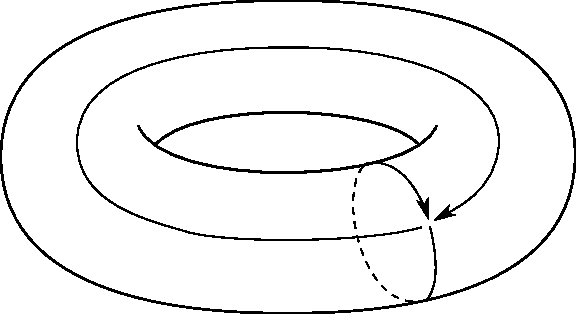
\includegraphics[width=2in]{905/Figures/01-torus-generating-cycles}
\end{center}

\medskip
We will learn to compute the homology groups of a wide variety of spaces. 
The $n$-sphere for example has the following homology groups:
\[
H_q(S^n)=\begin{cases}\ZZ & \hbox{if}\quad q=n>0\\
                \ZZ & \hbox{if}\quad q=0,n>0\\
                \ZZ\oplus\ZZ & \hbox{if}\quad q=n=0\\
                0 & \hbox{otherwise}\,.
\end{cases}
\]






%Some d^i and s^i fixed to d_i and s_i.
%Rhetorical questions are okay in spoken lectures but I think they should be used more sparingly in text.

\section{More about homology}
In the last lecture we introduced the standard $n$-simplex $\Delta^n\subseteq\mathbf{R}^{n+1}$. Singular simplices in a space $X$ are maps $\sigma\colon\Delta^n\to X$ and constitute the set $\Sin_n(X)$. For example, $\Sin_0(X)$ consists of points of $X$. We also described the face inclusions $d^i:\Delta^{n-1}\to\Delta^n$, and the induced ``face maps'' 
\[
d_i:\Sin_n(X)\to\Sin_{n-1}(X)\,,0\leq i\leq n\,,
\]
given by precomposing with face inclusions: $d_i\sigma=\sigma\circ d^i$. 
For homework you established some quadratic relations satisfied by these maps.
A collection of sets $K_n,n\geq0$, together with maps $d_i:K_n\to K_{n-1}$
related to each other in this way, is a {\em semi-simplicial set}. 
So we have assigned to any space $X$ a semi-simplicial set $S_*(X)$. 

To the semi-simplicial set $\{\Sin_n(X),d_i\}$ we then applied the free abelian group functor, obtaining a semi-simplicial abelian group. Using the $d_i$s, we constructed a boundary map $d$ which makes $S_\ast(X)$ a \emph{chain complex} -- that is, $d^2=0$. We capture this process in a diagram:
\begin{equation*}
\xymatrix{
\{\text{spaces}\}\ar[d]^{\Sin_*}\ar[r]^{H_*} & 
\{\text{graded abelian groups}\} \\
\{\text{semi-simplicial sets}\}\ar[d]^{\mathbf{Z}(-)} \\ 
\{\text{semi-simplicial abelian groups}\}\ar[r] & 
\{\text{chain complexes}\}\ar[uu]_{\text{take homology}}\\
}\end{equation*}
%Given a chain complex $\partial\colon A_n\to A_{n-1}$, one can define its homology $H_n(A,\partial)=\ker\partial_n/\img\partial_n$.

\begin{example} Suppose we have $\sigma\colon \Delta^1\to X$. Define $\phi\colon\Delta^1\to\Delta^1$ by sending $(t,1-t)$ to $(1-t,t)$. Precomposing $\sigma$ with $\phi$ gives another singular simplex $\overline{\sigma}$ which reverses the orientation of $\sigma$. It is \textit{not} true that $\overline{\sigma}=-\sigma$ in $S_1(X)$.

However, we claim that $\overline{\sigma}\equiv -\sigma\bmod B_1(X)$. This means that there is a $2$-chain in $X$ whose boundary is $\overline{\sigma}+\sigma$. If $d_0\sigma=d_1\sigma$, so that $\sigma\in Z_1(X)$, then $\overline{\sigma}$ and $-\sigma$ are homologous: $[\overline{\sigma}]=-[\sigma]$ in $ H_1(X)$.

To construct an appropriate boundary, consider the projection map 
$\pi:\Delta^2\to\Delta^1$ that is the affine extension of the map sending
$e_0$ and $e_2$ to $e_0$ and $e_1$ to $e_1$.  

\fbox{picture needed}
 
We'll compute $d(\sigma\circ\pi)$. Some of the terms will be constant
singular simplicies. Let's write $c_x^n:\Delta^n\to X$ for the constant map 
with value $x\in X$. Then
\[
d(\sigma\circ\pi)=\sigma\pi d^0-\sigma\pi d^1 +\sigma\pi d^2=\overline{\sigma}-c^1_{\sigma(0)}+\sigma\,.
\]
The constant simplex $c^1_{\sigma(0)}$ is an error term, and we wish to 
eliminate it. To achieve this we can use the constant $2$-simplex $c^2_{\sigma(0)}$ at $\sigma(0)$; its boundary is
\[
c^1_{\sigma(0)}-c^1_{\sigma(0)}+c^1_{\sigma(0)}=c^1_{\sigma(0)}\,.
\] 
So 
\[
\overline{\sigma}+\sigma=d(\sigma\circ\pi + c^2_{\sigma(0)})\,,
\] 
and $\overline{\sigma}\equiv -\sigma\bmod B_1(X)$ as claimed.

Some more language: two cycles that differ by a boundary $dc$ are said to be {\em homologous}, and the chain $c$ is a {\em homology} between them. 

\end{example}

Let's compute the homology of the very simplest spaces, $\varnothing$ and $\ast$. For the first , $\Sin_n(\varnothing)=\varnothing$, so $S_\ast(\varnothing)=0$. Hence $\cdots\to S_2\to S_1\to S_0$ is the zero chain complex. This means that $Z_\ast(\varnothing)=B_\ast(\varnothing)=0$. The homology in all dimensions is therefore $0$.

For $\ast$, we have $\Sin_n(\ast)=\{c^n_\ast\}$ for all $n\geq 0$. Consequently $S_n(\ast)=\mathbf{Z}$ for $n\geq0$ and $0$ for $n\leq0$. 
For each $i$, $d_ic^n_\ast=c^{n-1}_\ast$, so
the boundary maps $d\colon S_n(\ast)\to S_{n-1}(\ast)$ in the chain complex depend on the parity of $n$ as follows:
\[d(c^n_\ast)=\sum_{i=0}^{n}(-1)^i c^{n-1}_\ast=
\begin{cases}
    c^{n-1}_* & \text{for } n \text{ even, and}\\
    0 & \text{for } n \text{ odd.}
  \end{cases}
\]
This means that our chain complex is:
\[
0\leftarrow0\leftarrow\ZZ\xleftarrow{1}\ZZ\xleftarrow{0}\ZZ\xleftarrow{1}\cdots\,.\]
The boundaries coincide with the cycles except in dimension zero, where $B_0(\ast)=0$ while $Z_0(\ast)=\mathbf{Z}$. Therefore $ H_0(\ast)=\mathbf{Z}$ and $ H_i(\ast)=0$ for $i\neq0$.

We've defined homology groups for each space, but haven't yet considered what happens to maps between spaces. A continuous map $f\colon X\to Y$ induces a map $f_\ast\colon \Sin_n(X)\to\Sin_n(Y)$ by composition: 
\[
f_\ast:\sigma\mapsto f\circ \sigma\,.
\] 
For $f_\ast$ to be a map of semi-simplicial sets, it needs to commute with face maps. Explicitly, we need $f_\ast \circ d_i = d_i \circ f_\ast$. A diagram is said to be \emph{commutative} if all composites with the same source and target are equal, so this equation is equivalent to commutativity of the diagram
\begin{eqnarray*}
\xymatrix{\Sin_n(X)\ar[r]^{f_\ast}\ar[d]^{d_i} & \Sin_n(Y)\ar[d]^{d_i}\\
\Sin_{n-1}(X)\ar[r]^{f_\ast} & \Sin_{n-1}(Y)\,.}
\end{eqnarray*}
We see that $d_if_\ast\sigma=(f_\ast\sigma)\circ d^i=f\circ\sigma\circ d^i$, and $f_\ast(d_i\sigma)=f_\ast(\sigma\circ d^i)=f\circ\sigma\circ d^i$ as desired. The diagram remains commutative when we pass to the free abelian groups of chains.

If $C_\ast$ and $D_\ast$ are chain complexes, a \emph{chain map} $f\colon C_\ast\to D_\ast$ is a collection of maps $f_n\colon C_n\to D_n$ such that the following diagram commutes for every $n$:
\begin{equation*}
    \xymatrix{
	C_n\ar[r]^{f_n}\ar[d]^{d_C} & D_n\ar[d]^{d_D}\\
	C_{n-1}\ar[r]^{f_{n-1}} & D_{n-1}
    }
\end{equation*}
For example, if $f\colon X\to Y$ is a continuous map, then $f_\ast \colon S_\ast(X)\to S_\ast(Y)$ is a chain map as discussed above.

A chain map induces a map in homology $f_\ast: H_n(C)\to H_n(D)$. The method of proof is a so-called ``diagram chase'' and it will be the first of many. We check that we get a map $Z_n(C)\to Z_n(D)$. Let $c\in Z_n(C)$, so that $d_C c = 0$. Then $d_D f_n(c) = f_{n-1}d_C c = f_{n-1}(0) = 0$, because $f$ is a chain map. This means that $f_n(c)$ is also an $n$-cycle, i.e., $f$ gives a map $Z_n(C)\to Z_n(D)$.

Similarly, we also get a map $B_n(C)\to B_n(D)$. Let $c\in B_n(C)$, so that there exists $c^\prime \in C_{n+1}$ such that $d_C c^\prime = c$. Then $f_n(c) = f_nd_C c^\prime = d_D f_{n+1}(c^\prime)$. Thus $f_n(c)$ is the boundary of $f_{n+1}(c^\prime)$, and $f$ gives a map $B_n(C)\to B_n(D)$.

The two maps $Z_n(C)\to Z_n(D)$ and $B_n(C)\to B_n(D)$ quotient to give a map on homology $f_\ast: H_n(X)\to H_n(Y)$, as desired.

\section{Categories, functors, natural transformations}\label{categories}
%Office hours. Hood Chatham's are Mondays, 1:30 - 3:30, in 2-390A. Miller's is Tuesdays, 3:00-5:00 in 2-478. (commented out because not relevant to readers)
%Replaced \mathbf{C} with \cC as brought up in ``Stuff to fix.''
%Rearranged some stuff. Added a notational remark following the definition of a category.
From spaces and continuous maps, we constructed graded abelian groups and homomorphisms. We now cast this construction in the more general language of category theory.

Our discussion of category theory will be interspersed throughout the text, introducing new concepts as they are needed. Here we begin by introducing the basic definitions.

\begin{definition}
A \emph{category} $\cc$ consists of the following data.
\begin{itemize}
\item a class $\mathrm{ob}(\cc)$ of objects;
\item for every pair of objects $X$ and $Y$, a set of \emph{morphisms} 
$\cc(X,Y)$;
\item for every object $X$ a {\em identity morphism} $1_X\in\cc(X,X)$; and
\item for every triple of objects $X,Y,Z$, a {\em composition} map
$\cc(X,Y)\times\cc(Y,Z)\to\cc(X,Z)$, written $(f,g)\mapsto g \circ f$. 
\end{itemize}
These data are required to satisfy the following:
\begin{itemize}
\item $1_Y\circ f=f$, and $f\circ 1_X=f$.
\item Composition is associative: $(h\circ g)\circ f=h\circ(g\circ f)$.
\end{itemize}
\end{definition}
Note that we allow the collection of objects to be a class. This enables us to talk about a ``category of all sets'' for example. But we require each 
$\cc(X,Y)$ to be set, and not merely a class. Some interesting categories have
a {\em set} of objects; they are called {\em small categories}.

We will often write $X\in\cc$ to mean $X\in\mathrm{ob}(\cc)$, and $f\colon X\to Y$ to mean $f\in \cc(X,Y)$.
\begin{definition}
If $X,Y\in \cc$, then $f\colon X\to Y$ is an \emph{isomorphism} if there exists $g\colon Y\to X$ with $f \circ g=1_Y$ and $g\circ f=1_X$. We may write
\[
f:X\xrightarrow{\cong}Y
\]
to indicate that $f$ is an isomorphism. 
\end{definition}

\begin{example}
Many common mathematical structures can be arranged in categories.
\begin{itemize}
\item Sets and functions between them form a category $\set$.
\item Abelian groups and homomorphisms form a category $\mathbf{Ab}$.
\item Topological spaces and continuous maps form a category $\mathbf{Top}$.
\item Simplicial sets and their maps form a category $s\set$.
\item A monoid is the same as a category with one object, where the elements of the monoid are the morphisms in the category. It's a small category.
\item The sets $[n]=\{0,\ldots,n\}$ for $n\geq 0$ together with weakly order-preserving maps between them form the {\em simplex category} $\Deltab$, 
another small category. It contains as a subcategory the {\em semi-simplex
category} $\Deltab_{inj}$ with the same objects but only injective weakly order-preserving maps. 
\item A poset forms a category in which there is a morphism from $x$ to $y$ iff $x\leq y$. A small category with this property comes from a poset provided 
that the only isomorphisms are identities. 
\end{itemize}
\end{example}

Categories may be related to each other by rules describing effect on both
objects and morphisms. 
\begin{definition}
Let $\cc,\cd$ be categories. A \emph{functor} $F\colon\cc\to\cd$ consists
of the data of 
\begin{itemize}
\item an assignment  $F:\mathrm{ob}(\cc)\to\mathrm{ob}(\cd)$, and
\item for all $x,y\in\mathrm{ob}(\cc)$, map $F:\cc(x,y)\to\cc(F(x),F(y))$ \,.
\end{itemize}
These data are required to satisfy the following two properties:
\begin{itemize}
\item For all $X\in\mathrm{ob}\cc$, $F(1_X)=1_{F(X)}\in\cd(F(X),F(X))$, and
\item For all composable pairs of morphisms $f,g$ in $\cc$, 
$F(g\circ f)=F(g)\circ F(f)$.
\end{itemize}
\end{definition}

We have defined quite a few functors already:
\[
\Sin_n:\Top\to\mathbf{Set}\,,\quad S_n:\Top\to\Ab\,,\quad H_n:\Top\to\Ab\,,
\]
for example. We also have defined, for each $X$, 
a morphism $d:S_n(X)\to S_{n-1}(X)$. This is a ``morphism between 
functors.'' This property is captured by another definition.
\begin{definition}
Let $F,G\colon \cc\to\cd$. A \emph{natural transformation} 
or \emph{natural map} $\theta\colon F\to G$ consists of maps $\theta_X\colon F(X)\to G(X)$ for all $X\in\mathrm{ob}(\cc)$ such that for all $f\colon X\to Y$ the following diagram commutes. 
\begin{equation*}
\xymatrix{F(X)\ar[d]^{F(f)}\ar[r]^{\theta_X} & G(X)\ar[d]^{G(f)}\\
F(Y)\ar[r]^{\theta_Y} & G(Y)}
\end{equation*}
\end{definition}
So for example 
the boundary map $d\colon S_n\to S_{n-1}$ is a natural transformation.

Natural transformations are so \ldots well, so {\em natural} that their
occurance is indicated by a variety of terms: a {\em natural} or 
{\em canonical} map is precisely a natural transformation. 

\begin{example}
Suppose that $\cc$ and $\cd$ are two categories, and assume that $\cc$ is
small. We may then form the {\em category of functors} $\mathrm{Fun}(\cc,\cd)$.
Its objects are the functors fron $\cc$ to $\cd$, and given two functors
$F,G$, $\Fun(\cc,\cd)(F,G)$ is the set of natural transformations from $F$
to $G$. We let the reader define the rest of the structure of this category,
and check the axioms. We needed to assume that $\cc$ is small in order to
guarantee that there is no more than a set of natural transformations between
functors.

For example, let $G$ be a group (or a monoid) viewed as a one-object category. Any element $F\in\mathrm{Fun}(G,\mathbf{Ab})$ is simply a group action of $G$ on $F(\ast)=A$, i.e., a representation of $G$ in abelian groups. Given another $F^\prime\in\mathrm{Fun}(G,\mathbf{Ab})$ with $F^\prime(\ast)=A^\prime$, then a natural transformation from $F\to F^\prime$ is precisely a $G$-equivariant homomorphism $A\to A^\prime$.
\end{example}


\section{Categorical language}

Let $\mathrm{Vect}_k$ be the category of vector spaces over a field $k$, and linear transformations between them. Given a vector space $V$, you can consider the dual $V^\ast=\Hom(V,k)$. Does this give us a functor? If you have a linear transformation $f:V\to W$, you get a map $f^\ast:W^\ast\to V^\ast$, so this is like a functor, but the induced map goes the wrong way. This operation does preserve composition and identities, in an appropriate sense. This is an example of a {\em contravariant functor}. 

I'll leave it to you to spell out the definition, but notice that there is a univeral example of a contravariant functor out of a category $\cc$: $\cc\to\cc^{op}$, where $\cc^{op}$ has the same objects as $\cc$, but $\cc^{op}(X,Y)$ is declared to be the set $\cc(Y,X)$. The identity morphisms remain the same. To describe the composition in $\cc^{op}$, I'll write $f^{op}$ for $f\in\cc(Y,X)$ regarded as an element of $\cc^{op}(X,Y)$; then $f^{op}\circ g^{op}=(g\circ f)^{op}$. 

Then a contravariant functor from $\cc$ to $\cd$ is the same thing as a (``covariant'') functor from $\cc^{op}$ to $\cd$. 

Let $\cc$ be a category, and let $Y\in\mathrm{ob}(\cc)$. We get a map $\cc^{op}\to\mathbf{Set}$ that takes $X\mapsto \cc(X,Y)$, and takes a map $X\to W$ to the map defined by composition $\cc(W,Y)\to \cc(X,Y)$. This is called the functor {\em represented by} $Y$. It is very important to note that $\cc(-,Y)$ is contravariant, while, on the other hand, for any fixed $X$, $\cc(X,-)$ is a covariant functor (and is said to be ``corepresentable'' by $X$).

\begin{example}
Recall that the simplex category $\Deltab$ has objects the totally ordered sets
$[n]=\{0,1,\ldots,n\}$, with order preserving maps as morphisms. The ``standard simplex'' gives us a functor $\Delta\colon\Deltab\to\mathbf{Top}$. Now fix a space $X$, and consider 
\[
[n]\mapsto\mathbf{Top}(\Delta^n,X)\,.
\]
This gives us a contravariant functor $\Deltab\to\Set$, or a covariant
functor $\Deltab^{op}\to\Set$. This functor carries in it all the face and degeneracy maps we discussed earlier, and their compositions. Let us make a definition.
\end{example}

\begin{definition} Let $\cc$ be any category. A {\em simplicial object} in $\cc$ is a functor $K:\Deltab^{op}\to\cc$. Simplicial objects in $\cc$ form a category with natural transformations as morphisms. Similarly, {\em semi-simplicial object} in $\cc$ is a functor $\Deltab_{inj}^{op}\to\cc$,
\end{definition}

So the singular functor $\Sin_\ast$ gives a functor from spaces to simplicial sets (and so, by restriction, to semi-simplicial sets). 

I want to interject one more bit of categorical language that will often be useful to us. 

\begin{definition}
A morphism $f:X\to Y$ in a category $\cc$ is a \textit{split epimorphism} (``split epi'' for short) if there exists $g:Y\to X$ (called a section or a splitting) such that the composite $Y\xrightarrow{g}X\xrightarrow{f}Y$ is the identity.
\end{definition}
\begin{example}
In the category of sets, a map $f:X\to Y$ is a split epimorphism exactly when, 
for every element of $Y$ there exists some element of $X$ whose image in $Y$ is the original element. So $f$ is surjective. Is every surjective map a split epimorphism? This is equivalent to the axiom of choice! because a section of $f$ is precisely a choice of $x\in f^{-1}(y)$ for every $y\in Y$.
\end{example}
Every categorical definition is accompanied by a ``dual'' definition. 
\begin{definition}
A map $g:Y\to X$ is a {\em split monomorphism} (``split mono'' for short) if there is $f:X\to Y$ such that $f\circ g=1_Y$.
\end{definition}
\begin{example}
Again let $\cc=\Set$. Any split monomorphism is an injection: If $y,y^\prime\in Y$, and $g(y)=g(y^\prime)$, we want to show that $y=y^\prime$. Apply $f$, to get $y=f(g(y))=f(g(y^\prime))=y^\prime$. But the injection $\varnothing\to Y$ 
is a split monomorphism only if $Y=\varnothing$. So there's an asymmetry 
in the category of sets.
\end{example}
\begin{lemma}
A map is an isomorphism if and only if it is both a split epimorphism and a
split monomorphism.
\end{lemma}
\begin{proof}
Easy!
\end{proof}
The importance of these definitions is this: Functors will not in general
respect ``monomorphisms'' or ``epimorphisms,'' but:
\begin{lemma}
Any functor sends split epis to split epis and split monos to split monos.
\end{lemma}
\begin{proof}
Apply $F$ to the diagram establishing $f$ as a split epi or mono.
\end{proof}
\begin{example}
Suppose $\cc=\mathbf{Ab}$, and you have a split epi $f:A\to B$. Let $g:B\to A$ be a section. We also have the inclusion $i:\ker f\to A$, and hence a map
\[
[\,g\quad i\,]:B\oplus\ker f\to A\,.
\]
I leave it to you to check that this map is an isomorphism, and to formulate a
dual statement.
\end{example}

\section{Homotopy, star-shaped regions}

We've computed the homology of a point. Let's now compare the homology of
a general space $X$ to this example. There's always a unique map $X\to\ast$: $\ast$ is a ``terminal object'' in $\mathbf{Top}$. We have an induced map 
\[ 
H_n(X)\to H_n(\ast)=
\begin{cases}\mathbf{Z} & n=0\\
0 & \text{otherwise}\,.\end{cases}
\]
Any formal linear combination $c=\sum a_i x_i$ of points of $X$ is a 0-cycle. 
The map to $\ast$ sends $c$ to $\sum a_i\in\mathbf{Z}$. This defines
the {\em augmentation} $\epsilon:H_*(X)\to H_*(\ast)$. 
If $X$ is nonempty, the map $X\to\ast$ is split by any choice of point in $X$,
so the augmentation is also split epi. The kernel of $\epsilon$ is the 
{\em reduced homology} $\widetilde H_*(X)$ of $X$, and we get a canonical 
splitting 
\[
H_*(X)\cong \widetilde H_*(X)\oplus\mathbf{Z}\,.
\]

Actually, it's useful to extend the definition to the empty space by the
following device. Extend the singular chain complex for any space to include 
$\ZZ$ in dimension $-1$, with $d:S_0(X)\to S_{-1}(X)$ given by the 
augmentation $\epsilon$ sending each $0$-simplex to $1\in\ZZ$. 
Let's write $\widetilde S_*(X)$ for this chain 
complex, and $\widetilde H_*(X)$ for its homology. 
When $X\neq\varnothing$, $\epsilon$ is surjective
and you get the same answer as above. But 
\[
\widetilde H_q(\varnothing)=
\begin{cases}\mathbf{Z} & \hbox{for}\,q=-1\\0 & \hbox{for}\,q\neq-1\,.
\end{cases}
\]
This convention is not universally accepted, but I find it useful.
$\widetilde H_*(X)$ is the {\em reduced homology} of $X$.

What other spaces have trivial homology? A slightly non-obvious way to reframe
the question is this:
\begin{quote}
When do two maps $X\to Y$ induce the same map in homology? 
\end{quote}
For example,
when do $1_X:X\to X$ and $X\to\ast\to X$ induce the same map in homology?
If they do, then $\epsilon:H_*(X)\to\mathbf{Z}$ is an isomorphism. 

The key idea is that homology is a discrete invariant, so it should be 
unchanged by deformation. Here's the definition that makes ``deformation''
precise.
\begin{definition}
Let $f_0,f_1:X\to Y$ be two maps. A {\em homotopy} from $f_0$ to $f_1$ is a map $h:X\times I\to Y$ (continuous, of course) such that $h(x,0)=f_0(x)$ and $f(x,1)=f_1(x)$. We say that $f_0$ and $f_1$ are {\em homotopic}, and that $h$ is a {\em homotopy} between them. This relation is denoted by $f_0\simeq f_1$. 
\end{definition}
Homotopy is an equivalence relation on maps from $X$ to $Y$.
Transitivity follows from the gluing lemma of point set topology.
We denote by $[X,Y]$ the set of {\em homotopy classes} of maps from $X$ to $Y$.
A key result about homology is this:
\begin{theorem}[Homotopy invariance of homology]\label{thm-homotopy-invariance}
If $f_0\simeq f_1$, then $ H_\ast(f_0)= H_\ast(f_1)$: homology cannot distinguish between homotopic maps.
\end{theorem}
Suppose I have two maps $f_0,f_1:X\to Y$ with a homotopy $h:f_0\simeq f_1$, and a map $g:Y\to Z$. Composing $h$ with $g$ gives a homotopy between $g\circ f_0$ and $g\circ f_1$. Precomposing also works: If $g:W\to X$ is a map and $f_0,f_1:X\to Y$ are homotopic, then $f_0\circ g\simeq f_1\circ g$. This lets us compose homotopy classes: we can complete the diagram:
\begin{equation*}
\xymatrix{\mathbf{Top}(Y,Z)\times\mathbf{Top}(X,Y)\ar[d]\ar[r] & \mathbf{Top}(X,Z)\ar[d]\\
[Y,Z]\times[X,Y]\ar@{-->}[r] & [X,Z]}
\end{equation*}
\begin{definition}
The {\em homotopy category} (of topological spaces) 
$\mathrm{Ho}(\mathbf{Top})$ has the same objects as $\mathbf{Top}$, but
$\mathrm{Ho}(\mathbf{Top})(X,Y)=[X,Y]=\mathbf{Top}(X,Y)/\simeq$.
\end{definition}
We may restate Theorem \ref{thm-homotopy-invariance} as follows:
\begin{quote}
For each $n$,
the homology functor $ H_n:\mathbf{Top}\to\mathbf{Ab}$ factors as $\mathbf{Top}\to\mathrm{Ho}(\mathbf{Top})\to\mathbf{Ab}$; it is a ``homotopy functor.''
\end{quote}
We will prove this in the next lecture, but let's stop now and think about some
consequences. 
\begin{definition}
A map $f:X\to Y$ is a {\em homotopy equivalence} if $[f]\in[X,Y]$ is an isomorphism in $\htop$. In other words, there is a map $g:Y\to X$ such that $fg\simeq 1_Y$ and $gf\simeq1_X$. 
\end{definition}
Such a map $g$ is a {\em homotopy inverse} for $f$; it is well-defined
only up to homotopy.

Most topological properties are not preserved by homotopy equivalences.
For example, compactness is not a homotopy-invariant property: Consider the inclusion $i:S^{n-1}\subseteq \mathbf{R}^n-\{0\}$. A homotopy inverse $p:\mathbf{R}^n-\{0\}\to S^{n-1}$ can be obtained by dividing a (always nonzero!) vector by its length. Clearly $p\circ i=1_{S^{n-1}}$. We have to find a homotopy $i\circ p\simeq1_{\mathbf{R}^n-\{0\}}$. This is a map $(\mathbf{R}^n-\{0\})\times I\to \mathbf{R}^n-\{0\}$, and we can use $(v,t)\mapsto tv+(1-t)\frac{v}{||v||}$.

On the other hand:
\begin{corollary}
Homotopy equivalences induce isomorphisms in homology.
\end{corollary}
\begin{proof} 
If $f$ has homotopy inverse $g$, then $f_*$ has inverse $g_*$.
\end{proof}
\begin{definition}
A space $X$ is {\em contractible} if the map $X\to\ast$ is a homotopy equivalence.
\end{definition}
\begin{corollary}
Let $X$ be a contractible space. The augmentation $\epsilon:H_*(X)\to\mathbf{Z}$ is an isomorphism. 
\end{corollary}

Homotopy equivalences in general may be somewhat hard to visualize. 
A particularly simple and important class of homotopy equivalences is 
given by the following definition. 
\begin{definition}
An inclusion $A\hookrightarrow X$ is a {\em deformation retract} 
provided that there is a map $h:X\times I\to X$ such that 
$h(x,0)=x$ and $h(x,1)\in A$ for all $x\in X$ and $h(a,t)=a$ for all
$a\in A$ and $t\in I$. 
\end{definition}

For example, $S^{n-1}$ is a deformation retract of $\RR^n-\{0\}$.

\bigskip
We now set about constructing a proof of homotopy invariance of homology. 
The first step is to understand the analogue of homotopy on the level of
chain complexes. 
	\begin{definition}
	Let $C_\ast,D_\ast$ be chain complexes, and $f_0,f_1:C_\ast\to D_\ast$ be chain maps. A {\em chain homotopy} $h:f_0\simeq f_1$ is a collection of homomorphisms $h:C_n\to D_{n+1}$ such that $dh+hd=f_1-f_0$.
	\end{definition}
This relation takes some getting used to. It is an equivalence relation.
Here's a picture (not a commutive diagram).
\begin{equation*}\xymatrix{
\cdots \ar[r] & 
C_{n+1}\ar[d]\ar[r]^d & C_n\ar@{-->}[dl]_h\ar[d]\ar[r]^d &
C_{n-1}\ar@{-->}[dl]_h\ar[d]\ar[r] & \cdots \\
\cdots \ar[r] & D_{n+1}\ar[r]^d & D_n \ar[r]^d & D_{n-1}\ar[r] & \cdots
}\end{equation*}

\begin{lemma}
If $f_0,f_1:C_\ast\to D_\ast$ are chain homotopic, then 
$f_{0\ast}=f_{1\ast}: H_\ast(C)\to H_\ast(D)$.
	\end{lemma}
		\begin{proof}
We want to show that for every $c\in Z_n(C_\ast)$, the difference 
$f_1c-f_0c$ is a boundary. Well, 
\[
f_1c-f_0c=(d h+hd)c=d hc+hd c=dhc\,.
\]
		\end{proof}

So homotopy invariance of homology will follow from
\begin{prop}
Let $f_0,f_1:X\to Y$ be homotopic. Then $f_{0*},f_{1*}:S_\ast(X)\to S_\ast(Y)$ are chain homotopic.
\end{prop}

To prove this we will begin with a special case. 
\begin{definition}
A subset $X\subseteq\RR^n$ is {\em star-shaped} with respect to $b\in X$ if
for every $x\in X$ the interval 
\[
\{tb+(1-t)x:t\in[0,1]\}
\]
lies in $X$. 
\end{definition}

\begin{center}
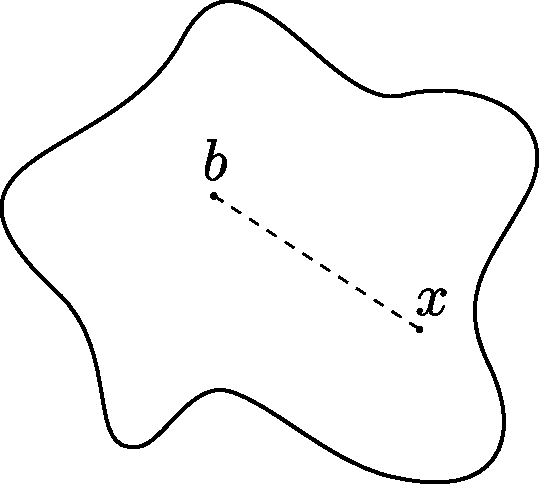
\includegraphics[width=2in]{905/Figures/05-star-shaped.pdf}
\end{center}

Any nonempty convex region is star shaped.
Any star-shaped region $X$ is contractible: A homotopy 
inverse to $X\to\ast$ is given by sending $\ast\mapsto b$. One composite is
perforce the identity. A homotopy from the other composite to the identity
$1_X$ is given by $(x,t)\mapsto tb+(1-t)x$.

So we should expect that $\epsilon:H_*(X)\to\mathbf{Z}$ is an isomorphism 
if $X$ is star-shaped. In fact, using a piece of language that the reader
can interpret:
\begin{prop}
$S_*(X)\to\mathbf{Z}$ is a chain homotopy equivalence.
\end{prop}

		\begin{proof}
		We have maps $S_\ast(X)\xrightarrow{\epsilon}\mathbf{Z}\xrightarrow{\eta}S_\ast(X)$ where $\eta(1)=c_b^0$. Clearly $\epsilon\eta=1$, and the claim is that $\eta\epsilon\simeq1:S_\ast(X)\to S_\ast(X)$. The chain map 
$\eta\epsilon$ concentrates everything at the point $b$: 
$\eta\epsilon\sigma=c_b^n$ for all $\sigma\in\Sin_n(X)$. 
Our chain homotopy $h:S_q(X)\to S_{q+1}(X)$ will actually send simplices to simplices. For $\sigma\in\Sin_q(X)$, define the chain homotopy evaluated on $\sigma$ by means of the following ``cone construction'': $h(\sigma)=b*\sigma$, where
\[
(b*\sigma)(t_0,\ldots,t_{q+1})=t_0b+(1-t_0)\sigma\left(\frac{(t_1,\ldots,t_{q+1})}{1-t_0}\right)\,.
\]
Explanation: The denominator $1-t_0$ makes the entries sum to 1, as they must if we are to apply $\sigma$ to this vector. When $t_0=1$, this isn't defined, but it doesn't matter since we are multiplying by $1-t_0$. So
$(b*\sigma)(1,0,\ldots,0)=b$; this is the vertex of the cone. 

\begin{center}
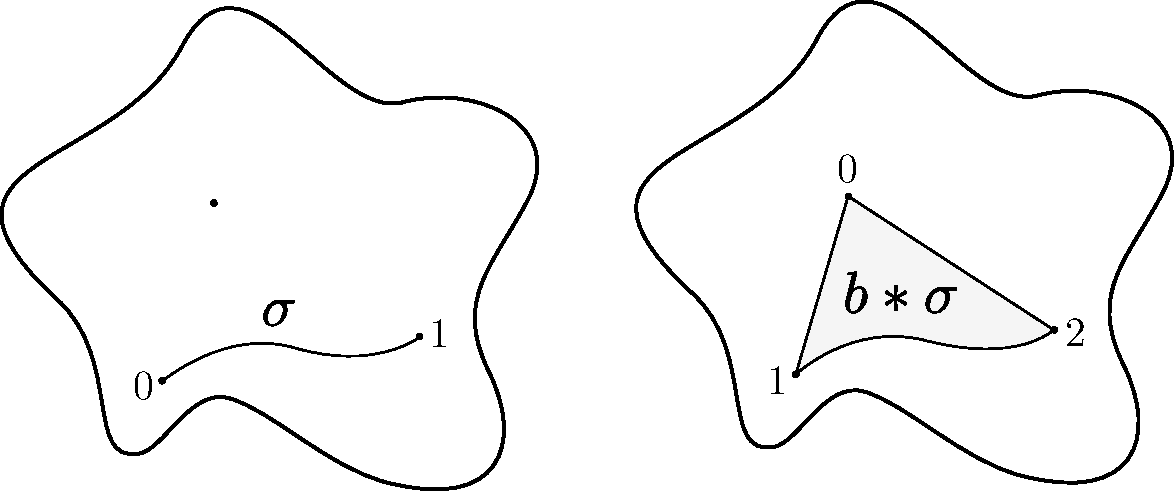
\includegraphics[width=5in]{905/Figures/05-homotopy.pdf}
\end{center}

Setting $t_0=0$, we find
\[
d_0b*\sigma=\sigma\,.
\]
Setting $t_i=0$ for $i>0$, we find
\[
d_ib*\sigma=hd_{i-1}\sigma\,.
\]
Using the formula for the boundary operator, we find
\[
db*\sigma=\sigma-b*d\sigma
\]
\ldots {\em unless} $q=0$, when 
\[
db*\sigma=\sigma-c_b^0\,.
\]
This can be assembled into the equation
\[
db*+b*d=1-\eta\epsilon
\]
which is what we wanted. 		
\end{proof}




% Continue indenting like this.

\section{Homotopy invariance of homology}
We now know that the homology of a star-shaped region is trivial: in such a space, every cycle with augmentation 0 is a boundary. We will use that fact, which is a special case of homotopy invariance of homology, to prove the general result, which we state in somewhat stronger form:
	\begin{theorem}
A homotopy $h:f_0\sim f_1:X\to Y$ determines a natural chain homotopy
$f_{0,\ast}\sim f_{1,\ast}:S_\ast(X)\to S_\ast(Y)$.
	\end{theorem}

The proof uses naturality (a lot). For a start, notice that if $k:g_0\sim g_1:C_*\to D_*$ is a chain homotopy, and $j:D_*\to E_*$ is another chain map, then the composites $j\circ k_n:C_n\to E_{n+1}$ give a chain homootpy $j\circ g_0\sim j\circ g_1$. So if we can produce a chain homotopy homotopy between the chain maps induced by the two inclusions $i_0,i_1:X\to X\times I$, we can get a chain homotopy $k$ between $f_{0*}=h_*\circ i_{0*}$ and 
$f_{1*}=h_*\circ i_{1*}$ in the form $h_*\circ k$. 

So now we want to produce a natural chain homotopy, with components 
$k_n:S_n(X)\to S_{n+1}(X\times I)$. The unit interval hosts a natural 1-simplex
given by an identification $\Delta^1\to I$, and we should imagine $k$ as being
given by ``multiplying'' by that 1-chain. This ``multiplication'' is a special
case of a chain map 
\[
\times:S_*(X)\times S_*(Y)\to S_*(X\times Y)\,,
\]
defined for any two spaces $X$ and $Y$, 
with lots of good properties. It will ultimately be used to compute the homology of a product of two spaces in terms of the homology groups of the factors. 

Here's the general result. 
\begin{theorem}
There exists a map $S_p(X)\times S_q(Y)\to S_{p+q}(X\times Y)$ that is:
	\begin{itemize}
	\item Natural, in the sense that if $f:X\to X^\prime$ and $g:Y\to Y^\prime$, and $a\in S_p(X)$ and $b\in S_p(Y)$ so that $a\times b\in S_{p+q}(X\times Y)$, then $f_\ast(a)\times g_\ast(b)=(f\times g)_\ast(a\times b)$.
	\item Bilinear, in the sense that $(a+a^\prime)\times b=(a\times b)+(a^\prime\times b)$, and $a\times (b+b^\prime)=a\times b+a\times b^\prime$.
	\item The Leibniz rule is satisfied, i.e., $d(a\times b)=(da)\times b + (-1)^pa\times db$.
	\item Normalized, in the following sense. Let $x\in X$ and $y\in Y$. Write $j_x:Y\to X\times Y$ sending $y\mapsto (x,y)$, and write $i_y:X\to X\times Y$ sending $x\mapsto (x,y)$. If $b\in S_q(Y)$, then $c^0_x\times b=(j_x)_\ast b\in S_q(X\times Y)$, and if $a\in S_p(X)$, then $a\times c^0_y=(i_y)_\ast a\in S_p(X\times Y)$.
	\end{itemize}
\end{theorem}
The Leibniz rule contains the first occurence of the ``topologists sign rule'';
we'll see these signs appearing often. Watch for when it appears in our proof.

\begin{proof} We're going to use induction on $p+q$; the normalization axiom 
gives us the cases $p+q=0,1$. Let's assume that we've constructed the cross-product in total dimension $p+q-1$. We want to define $\sigma\times\tau$ for 
$\sigma\in S_p(X)$ and $\tau\in S_q(Y)$. 

Note that there's a universal example of a $p$-simplex, namely the identity map $\iota_p:\Delta^p\to \Delta^p$. It's universal in the sense that given any $p$-simplex $\sigma:\Delta^p\to X$, you get $\sigma=\sigma_\ast(\iota_p)$ where $\sigma_\ast:\Sin_p(\Delta^p)\to \Sin_p(X)$ is the map induced by $\sigma$. To define $\sigma\times\tau$ in general, then, it suffices to define $\iota_p\times\iota_q\in S_{p+q}(\Delta^p\times\Delta^q)$; we can (and must) then take
$\sigma\times\tau=(\sigma\times\tau)_*(\iota_p\times\iota_q)$. 

Our long list of axioms is useful in the induction. For one thing, if $p=0$ or
$q=0$, normalization provides us with a choice. So now assume that both $p$ and $q$ are positive. We want the cross-product
to satisfy the Leibnitz rule: 
		\begin{equation*}
d(\iota_p\times\iota_q) = (d\iota_p)\times\iota_q + (-1)^p\iota_p\times d\iota_q\in		S_{p+q-1}(\Delta^p\times\Delta^q)
		\end{equation*}
Since $d^2=0$, a necessary condition for $\iota_p\times\iota_q$ to exist is that $d((d\iota_p)\times\iota_q + (-1)^p\iota_p\times d\iota_q) =0$. Let's compute what this is, using the Leibnitz rule in dimension
$p+q-1$ where we have it by the inductive assumption:
		\begin{equation*}
		d((d\iota_p)\times\iota_q + (-1)^p\iota_p\times(d\iota_q)) = (d^2\iota_p)\times\iota_q + (-1)^{p-1}(d\iota_p)\times(d\iota_q) + (-1)^p(d\iota_p)\times d\iota_q + (-1)^q\iota_p\times(d^2\iota_q) = 0
		\end{equation*}
because $d^2=0$. Note that this calculation would not have worked without the sign! 

The subspace $\Delta^p\times\Delta^q\subseteq\mathbf{R}^{p+1}\times\mathbf{R}^{q+1}$ is convex, so by translation, it's homeomorphic to a star-shaped region. Therefore we know that $ H_{p+q-1}(\Delta^p\times\Delta^q)=0$ (remember, $p+q>1$), which means that every cycle is a boundary. In other words, our necessary condition is also sufficient! So, choose any element 
with the right boundary and declare it to be $\iota_p\times\iota_q$.

The induction is now complete provided we can check that this choice satisfies naturality, bilinearity, and the Leibniz rule. We leave this as a relaxing exercise for the reader. 
\end{proof}

The essential point here is that the space supporting the universal pair of
simplices -- $\Delta^p\times\Delta^q$ -- has trivial homology. Naturality 
transports the result of that fact to the general situation. 
 
The cross-product that this procedure constructs is not unique; it depends on a choice a choice of the chain $\iota_p\times\iota_q$ for each pair $p,q$ with $p+q>1$. The cone construction in the proof that star-shaped regions have vanishing homology provids us with a specific choice; but it turns out that any two choices are equivalent up to natural chain homotopy. 

We return to homotopy invariance. To define our chain homotopy
$h_X:S_n(X)\to S_{n+1}(X\times I)$, pick any 1-simplex $\iota:\Delta^1\to I$
such that $d_0\iota=1$ and $d_1\iota=0$, and define
\[
h_X\sigma =(-1)^n\sigma\times\iota\,.
\]
Let's compute:
		\begin{equation*}
		dh_X\sigma =(-1)^nd(\sigma\times \iota) = 
(-1)^n(d\sigma)\times\iota + \sigma\times(d\iota)
		\end{equation*}
But $d\iota = c_1^0 - c_0^0\in S_0(I)$, 
which means that we can continue (remembering that $|\partial\sigma|=n-1$):
\[
=-h_X d\sigma+(\sigma\times c_1^0-\sigma\times c_0^0)
=-h_X d\sigma+(\iota_{1*}\sigma-\iota_{0*}\sigma)\,,
\]
using the normalization axiom of the cross-product. This is the result.



\section{Homology cross product}

In the last lecture we proved homotopy invariance of homology using the
construction of a chain level bilinear cross-product
\[
\times:S_p(X)\times S_q(Y)\to S_{p+q}(X\times Y)
\]
that satisfied the Leibniz formula
\[
d(a\times b)=(da)\times b+(-1)^pa\times(db)\,
\]
What else does this map give us? 

Let's abstract a little bit. Suppose we have three chain complexes $A_*$, $B_*$, and $C_*$, and suppose we have maps $\times: A_p\times B_q\to C_{p+q}$ that satisfy bilinearity and the Leibniz formula. What does this induce in homology?
\begin{lemma}
This determines a bilinear map $ H_p(A)\times H_q(B)\xrightarrow{\times} H_{p+q}(C)$.
\end{lemma}
\begin{proof}
Let $a\in Z_p(A)$ and $b\in Z_q(A)$. We want to define $[a]\times [b]\in H_{p+q}(C)$. We hope that $[a]\times [b]=[a\times b]$. We need to check that $a\times b$ is a cycle. By Leibniz, $d(a\times b)=da\times b+(-1)^pa\times db$. Because $a,b$ are boundaries, this is zero. Now we need to check that this thing is well-defined. Let's pick other cycles $a^\prime$ and $b^\prime$ in the same homology classes. We want $[a\times b]=[a^\prime\times b^\prime]$. In other words, we need to show that $a\times b$ differs from $a^\prime\times b^\prime$ by a boundary. We can write $a^\prime=a+d\overline{a}$ and $b^\prime=b+d\overline{b}$, and compute, using bilinearity:
	\begin{equation*}
	a^\prime\times b^\prime=(a+d\overline{a})+(b+d\overline{b})
	= a\times b+a\times d\overline{b} + (d\overline{a})\times b+(d\overline{a})\times(d\overline{b})
	\end{equation*}
We need to deal with the last three terms here. But since $da=0$,
\[
d(a\times\overline b)=(-1)^pa\times(d\overline b)\,.
\]
Since $d\overline b=0$, 
\[
d((\overline a)\times b)=(d\overline a)\times b\,.
\]
And since $d^2\overline b=0$, 
\[ 
d(a\times\overline{b})=
(d\overline a)\times(d\overline{b})\,.
\]
This means that $a^d\times b^d$ and $a\times b$ differ by 
\[
d((-1)^p(a\times \overline{b}) + \overline{a}\times b + \overline{a}\times d\overline{b})\,,
\]
and so are homologous. 

The last step is to check bilinearity, which is left to the reader.
\end{proof}
This gives the following result.
\begin{theorem}
There is a map 
\[
\times:H_p(X)\times H_q(Y)\to H_{p+q}(X\times Y)
\]
that is natural, bilinear, and normalized. 
\end{theorem}

This map is also \emph{uniquely defined} by these conditions, unlike the chain-level cross product.

I just want to mention an explicit choice of $\iota_p\times\iota_q$. This is called the Eilenberg-Zilber chain. You're highly encouraged to think about this yourself. It comes from a triangulation of the prism. 

The simplices in this triangulation are indexed by order preserving injections
\[
\omega:[p+q]\to[p]\times[q]
\]
Injectivity forces $\omega(0)=(0,0)$ and $\omega(p+q)=(p,q)$. Each such map
determines an affine map $\Delta^{p+q}\to\Delta^p\times\Delta^q$ of the same name. These will be
the singular simplices making up $\iota_p\times\iota_q$. To specify the coefficients, think of $\omega$ as a staircase in the rectangle $[0,p]\times[0,q]$. 
Let $A(\omega)$ denote the area under that staircase. Then the Eilenberg-Zilber chain is given by 
\[
\iota_p\times\iota_q=\sum(-1)^{A(\omega)}\overline{\omega}
\]

This description is in a paper by Eilenberg and Moore. 
It's very pretty, but it's combinatorially annoying to check that this satisfies the conditions of the theorem. It provides an explicit chain map
\[
\beta_{X,Y}:S_*(X)\times S_*(Y)\to S_*(X\times Y)
\]
that satisfies many good properties on the nose and not just up to chain homotopy. For example, it's {\em associative} --
\[
\xymatrix{
S_*(X)\times S_*(Y)\times S_*(Z) \ar[r]^{\beta_{X,Y}\times 1} 
\ar[d]^{1\times\beta{Y,Z}} & 
S_*(X\times Y)\times S_*(Z) \ar[d]^{\beta_{X\times Y,Z}} \\
S_*(X)\times S_*(Y\times Z) \ar[r]^{\beta_{X,Y\times Z}} &
S_*(X\times Y\times Z)
}\]
commutes -- and {\em commutative} --
\[
\xymatrix{
S_*(X)\times S_*(Y) \ar[r]^{\beta_{X,Y}} \ar[d]^{T} & 
S_*(X\times Y) \ar[d]^{S_*(T)} \\
S_*(Y)\times S_*(X) \ar[r]^{\beta_{Y,X}} \ar[r] & S_*(X\times Y)
}\]
commutes, where on spaces $T(x,y)=(y,x)$, and on chain complexes
$T(a,b)=(-1)^{pq}(b,a)$ when $a$ has degree $p$ and $b$ has degree $q$. 

We will see that these properties hold up to chain homotopy for any 
choice of chain-level cross product.


\section{Relative homology}

An ultimate goal of algebraic topology is to find means to compute the set of homotopy classes of maps from one space to another. This is important because many geometrical problems can be rephrased as such a computation. It's a lot more modest than wanting to characterize, somehow, all continuous maps from $X$ to $Y$; but the very fact that it still contains a great deal of interesting information means that it is still very challenging to compute. 

Homology is in a certain sense the best ``additive'' approximation to this problem; and its additivity makes it much more computable. To justify this, we want to describe the sense in which homology is ``additive.'' Here are two related aspects of this claim.
	\begin{enumerate}
	\item If $A\subseteq X$ is a subspace, then $ H_\ast(X)$ a combination of $ H_\ast(A)$ and $H_\ast(X-A)$. 
	\item The homology $ H_\ast(A\cup B)$ is like $ H_\ast(A)+ H_\ast(B)- H_\ast(A\cap B)$. 
	\end{enumerate}
The first hope is captured by the long exact sequence of a pair, the second
by the Meyer-Vietoris Theorem. 
Both facts show that homology behaves like a measure. 
The precise statement of both facts uses the machinery of exact sequences.
We'll use the following language.

\begin{definition}
A {\em sequence} of abelian groups is a diagram of abelian groups of the form 
\[
\cdots\rightarrow C_{n+1}\xrightarrow{f_n}C_n\xrightarrow{f_{n-1}}C_{n-1}
\rightarrow\cdots\,,
\]
finite or infinite in either or direction or both directions, in which all composites are zero; that is, $\img f_n\subseteq f_{n-1}$ for all $n$. It is 
{\em exact} at $C_n$ provided that this inequality is an equality. 
\end{definition}
\begin{example}
A sequence infinite in both directions is just a chain complex; it is exact at 
$C_n$ if and only if $H_n(C_\ast)=0$. So homology measures the failure of exactness.
\end{example}
\begin{example}
$0\to A\xrightarrow{i}B$ is exact iff $i$ is injective, and $B\xrightarrow{p}C\to 0$ is exact iff $p$ is surjective.
\end{example}
Exactness is a key property in the development of algebraic topology, and ``exact'' is a great word for the concept. A foundational treatment of algebraic topology was published by Sammy Eilenberg and Norman Steenrod published in 1952.
The story is that in the galleys for the book they left a blank space whenever the word representing this concept was used, and filled it in at the last minute. 
\begin{definition}
An exact sequence that's infinite in both directions
is a {\em long exact sequence}.
A {\em short exact sequence} is an exact sequence of the form 
\[
0\to A\xrightarrow{i}B\xRightarrow{p} C\to 0\,.
\]
\end{definition}

Any sequence of the form $0\to A\to B\to C\to0$ expands to a diagram
	\begin{equation*}
	\xymatrix{\ker(p) \ar[dr] & & \\
	A\ar[u]\ar[r]^i & B\ar[r]^p\ar[dr] & C\\
	 & & \coker(i)\ar[u]}
	\end{equation*}
It is short exact if and only if $A\rightarrow^{\cong}\ker p$ and 
$B\rightarrow^{\cong}\coker(i)$. 

As suggested above, we will study the homology of a space $X$ by comparing it to the homology of a subspace $A$ and a complement or quotient construction. 
Note that $S_*(A)$ injects into $S_*(X)$. This suggests considering the quotient group
\[
\frac{S_n(X)}{S_n(A)}\,.
\]
This is the group of {\em relative $n$-chains} of the pair $(X,A)$. 

Let's formalize this a bit. Along with the category $\mathbf{Top}$ of spaces,
we have the category $\mathbf{Top_2}$ of {\em pairs} of spaces. An object of
$\mathbf{Top_2}$ is a space $X$ together with a subspace $A$. A map
$(X,A)\to(Y,B)$ is a continuous map $X\to Y$ that sends $A$ into $B$. 

There are four obvious functors relating $\mathbf{Top}$ and $\mathbf{Top_2}$:
\[
X\mapsto(X,\varnothing)\,,\quad X\mapsto(X,X)\,,
\]
\[
(X,A)\mapsto X\,,\quad(X,A)\mapsto A\,.
\]

Do the relative chains form themselves into a chain complex? 
\begin{lemma}
Let $A_*$ be a subcomplex of the chain complex $B_*$. There is a unique
structure of chain complex on the quotient graded abelian group $C_*$ with 
entries $C_n=B_n/A_n$ such that $B_*\to C_*$ is a chain map.
\end{lemma}
\begin{proof}
To define $d:C_n\to C_{n-1}$, represent $c\in C_n$ by $b\in B_n$ and
hope that $[db]\in B_{n-1}/A_{n-1}$ is well defined. If we replace
$b$ by $b+a$ for $a\in A_n$, we find 
\[
d(b+a)=db+da\equiv da\mod A_{n-1}\,,
\]
so our hope is justified. Then $d^2[b]=[d^2 b]=0$. 
\end{proof}

\begin{definition} The {\em relative singular chain complex} of the pair 
$(X,A)$ is 
\[
S_*(X,A)=\frac{S_*(X)}{S_*(A)}\,.
\]
\end{definition}
This is a functor from pairs of spaces to chain complexes. Of course
\[
S_*(X,\varnothing)=S_*(X)\,,\quad S_*(X,X)=0\,.
\]

\begin{definition} The {\em relative singular homology} of the pair $(X,A)$
is the homology of the relative singular chain complex:
\[
H_n(X,A)=H_n(S_*(X,A))\,.
\]
\end{definition}

One of the nice features of the absolute chain group $S_n(X)$ is that it is free as an abelian group. Is that also the case for its quotent $S_n(X,A)$? The map $\Sin_n(A)\to\Sin_n(X)$ is an injection. As long as $A\neq\varnothing$, this injection admits a splitting. (If $A=\varnothing$, then $S_n(X,A)=S_n(X)$ is indeed free.) So when we apply the free abelian group functor we obtain a split monomorphism. Then the induced map $S_*(X)\to S_*(A)\oplus S_*(X,A)$ is an isomorphism, so $S_*(X,A)$ is again free. 

\begin{example}
Consider $\Delta^n$, relative to its boundary $\partial\Delta^n:=\bigcup \img d_i\cong S^{n-1}$. We have the identity map $\iota_n:\Delta^n\to \Delta^n$, the universal $n$-simplex, in $\Sin_n(\Delta^n)\subseteq S_n(\Delta^n)$. It is not a cycle; its boundary $d\iota_n\in S_{n-1}(\Delta^n)$ is the alternating sum of the faces of the $n$-simplex. Each of these singular simplices lies in $\partial\Delta^n$, so $d\iota_n\in S_{n-1}(\partial\Delta^n)$, and 
$[\iota_n]\in S_n(\Delta_n,\partial\Delta_n)$ {\em is} a {\em relative} cycle. 
We will see that the relative homology $H_n(\Delta^n,\partial\Delta^n)$ is infinite cyclic, with generator $[\iota_n]$. 
\end{example}

\section{The homology long exact sequence}

A pair of spaces $(X,A)$ gives rise to a short exact sequence of chain 
complexes:
\[
0\to S_*(A)\to S_*(X)\to S_*(X,A)\to0\,.
\]
In homology, this will relate $H_*(A)$, $H_*(X)$, and $H_*(X,A)$. 

To investigate what happens, let's suppse we have a general short exact 
sequence of chain complexes,
\[
0\to A_*\to B_*\to C_*\to0\,,
\]
and investigate what happens in homology. 

Here is an expanded part of this short exact sequence:
\begin{equation*}
\xymatrix{0\ar[r] & A_{n+1}\ar[r]^f\ar[d]^d & B_{n+1}\ar[r]^g\ar[d]^d & C_{n+1}\ar[r]\ar[d]^d & 0\\
0\ar[r] & A_n\ar[r]^f\ar[d]^d & B_n\ar[r]^g\ar[d]^d & C_n\ar[r]\ar[d]^d & 0\\
0\ar[r] & A_{n-1}\ar[r]^f & B_{n-1}\ar[r]^g & C_{n-1}\ar[r] & 0}
\end{equation*}
Clearly the composite $H(A_*)\to H_*(X)\to H_*(C)$ is trivial. Is this sequence
exact?  
Let $[b]\in H_n(B)$ such that $g([b])=0$. It's determined by some $b\in B_n$ such that $d(b)=0$. If $g([b])=0$, then there is some $\overline{c}\in C_{n+1}$ such that $d\overline{c}=gb$. Now, $g$ is surjective, so there is some $\overline{b}\in B_{n+1}$ such that $g(\overline{b})=\overline{c}$. Then we can consider $d\overline{b}\in B_n$, and $g(d(\overline{b}))=d(\overline{c})\in C_n$. What is $b-d\overline{b}$? This maps to zero in $C_n$, so by exactness there is some $a\in A_n$ such that $f(a)=b-d\overline{b}$. Is $a$ a cycle? Well, $f(da)=d(fa)=d(b-d\overline{b})=db-d^2\overline{b}=db$, but we assumed that $db=0$, so $f(da)=0$. This means that $da$ is zero because $f$ is an injection by exactness. Therefore $a$ is a cycle. What is $[a]\in H_n(A)$? Well, $f([a])=[b-d\overline{b}]=[b]$ because $d\overline{b}$ is a cycle. Is the composite $ H_n(A)\to H_n(B)\to H_n(C)$ zero? Yes, because the composite factors through zero. This proves exactness of $ H_n(A)\to H_n(B)\to H_n(C)$.

On the other hand, $H_*(A)\to H_*(B)$ may fail to be injective, and 
$H_*(B)\to H_*(C)$ may fail to be surjective. Instead:

\begin{theorem}[homology long exact sequence]
Let $0\to A_\ast\to B_\ast\to C_\ast\to 0$ be a short exact sequence of chain complexes. Then there is a natural homomorphism $\partial: H_n(C)\to H_{n-1}(A)$ such that the sequence 
\begin{equation*}
\xymatrix{ & \cdots \ar[r] & H_{n+1}(C) \ar[dll] \\
 H_n(A)\ar[r] & H_n(B)\ar[r] & H_n(C)\ar[dll]_\partial\\
 H_{n-1}(A)\ar[r] & \cdots & }
\end{equation*}
is exact.
\end{theorem}
\begin{proof}
We'll construct $\partial$, and leave the rest as an exercise. Again:
\begin{equation*}
\xymatrix{0\ar[r] & A_{n+1}\ar[r]^f\ar[d]^d & B_{n+1}\ar[r]^g\ar[d]^d & C_{n+1}\ar[r]\ar[d]^d & 0\\
0\ar[r] & A_n\ar[r]^f\ar[d]^d & B_n\ar[r]^g\ar[d]^d & C_n\ar[r]\ar[d]^d & 0\\
0\ar[r] & A_{n-1}\ar[r]^f & B_{n-1}\ar[r]^g & C_{n-1}\ar[r] & 0}
\end{equation*}
Let $c\in C_n$ such that $dc=0$. The map $g$ is surjective, so pick a $b\in B_n$ such that $g(b)=c$. Then consider $db\in B_{n-1}$. But $g(d(b))=0=d(g(b))=dc$. So by exactness, there is some $a\in A_{n-1}$ such that $f(a)=db$. How many choices are there of picking $a$? One, because $a$ is injective. We need to check that $a$ is a cycle. What is $d(a)$? Well, $d^2b=0$, so $da$ maps to $0$ under $f$. But because $f$ is injective, $da=0$, i.e., $a$ is a cycle. This means we can define $\partial[c]=[a]$.

To make sure that this is well-defined, let's make sure that this choice of homology class $a$ didn't depend on the $b$ that we chose. Pick some other $b^\prime$ such that $g(b^\prime)=c$. Then there is $a^\prime\in A_{n-1}$ such that $f(a^\prime)=db^\prime$. We want $a-a^\prime$ to be a boundary, so that $[a]=[a^\prime]$. We want $\overline{a}\in A_n$ such that $d\overline{a}=a-a^\prime$. Well, $g(b-b^\prime)=0$, so by exactness, there is $\overline{a}\in A_n$ such that $f(\overline{a})=b-b^\prime$. What is $d\overline{a}$? Well, $d\overline{a}=d(b-b^\prime)=db-db^\prime$. But $f(a-a^\prime)=b-b^\prime$, so because $f$ is injective, $d\overline{a}=a-a^\prime$, i.e., $[a]=[a^\prime]$. What else do I have to check? It's an exercise to check that $\partial$ as defined here is a homomorphism. Also, left as an exercise to check that this doesn't depend on $c\in[c]$, and that $\partial$ actually makes the exact sequence above exact.
\end{proof}

\begin{example} A pair of spaces $(X,A)$ gives rise to a natural long exact 
sequence in homology:
\begin{equation*}
\xymatrix{ 
& \cdots \ar[r] & H_{n+1}(X,A) \ar[dll]_\partial\\
 H_n(A)\ar[r] & H_n(X)\ar[r] & H_n(X,A)\ar[dll]_\partial\\
 H_{n-1}(A)\ar[r] & \cdots & 
}\,.
\end{equation*}
\end{example}

\begin{example} Let's think again about the pair $(D^n,S^{n-1})$. By homotopy invariance we know that $H_q(D^n)=0$ for $q>0$, since $D^n$ is contractible. So 
\[
\partial:H_q(D^n,S^{n-1})\to H_{q-1}(S^{n-1})
\] 
is an isomorphism for $i>1$. The bottom of the long exact sequence looks like 
this: 
\[
\xymatrix{
& 0 \ar[r] & H_1(D^n,S^{n-1}) \ar[lld] \\
H_0(S^{n-1}) \ar[r] & H_0(D^n) \ar[r] & H_0(D^n,S^{n-1}) \ar[r] & 0
}\]
When $n>1$, both $S^{n-1}$ and $D^n$ are path-connected, so the map
$H_0(S^{n-1})\to H_0(D^n)$ is an isomorphism, and 
\[
H_1(D^n,S^{n-1})=H_0(D^n,S^{n-1})=0\,.
\]
When $n=1$, we discover that
\[
H_1(D^1,S^0)=\mathbf{Z} \quad\hbox{and}\quad H_0(D^1,S^0)=0\,.
\]
The generator of $H_1(D^1,S^0)$ is represented by any 1-simplex 
$\iota_1:\Delta^1\to D^1$ such that $d_0\iota=1$ and $d_1\iota=0$ (or vice 
versa). 
To go any further in this analysis, we'll need another tool, known as
``excision.'' 
\end{example}

We can set this up for reduced homology (as in Lecture 5) as well. 
Note that any map induces an isomorphism in $\widetilde S_{-1}$, so to
a pair $(X,A)$ we can associate a short exact sequence
\[
0\to\widetilde S_*(A)\to\widetilde S_*(X)\to S_*(X,A)\to0
\]
and hence a long exact sequence 
\begin{equation*}
\xymatrix{ 
& \cdots \ar[r] & H_{n+1}(X,A)\ar[dll]_\partial\\
\widetilde H_n(A)\ar[r] & \widetilde H_n(X)\ar[r] & H_n(X,A)\ar[dll]_\partial\\\widetilde H_{n-1}(A)\ar[r] & \cdots &
}\,.
\end{equation*}

The homology long exact sequence is often used in conjunction with 
an elementary fact about a map between exact sequences known as the 
{\em five lemma}.
Suppose you have two exact sequences of abelian groups and a map between them
-- a ``ladder'':
\begin{equation*}
\xymatrix{A_4\ar[r]^d\ar[d]^{f_4} & A_3\ar[r]^d\ar[d]^{f_3} & A_2\ar[r]^d\ar[d]^{f_2} & A_1\ar[r]^d\ar[d]^{f_1} & A_0\ar[d]^{f_0}\\
B_4\ar[r]^d & B_3\ar[r]^d & B_2\ar[r]^d & B_1\ar[r]^d & B_0}
\end{equation*}
When can we guarantee that $f_2$ is an isomorphism? We're going to ``diagram chase.'' Just follow your nose, making assumptions as necessary.

Surjectivity:
Let $b_2\in B_2$. We want to show that there is something in $A_2$ mapping to $b_2$. We can consider $db_2\in B_1$. Let's assume that $f_1$ is surjective. Then there's $a_1\in A_1$ such that $f_1(a_1)=db_2$. What is $da_1$? Well, $f_0(da_1)=d(f_1(a_1))=d(db)=0$. So we want $f_0$ to be injective. Then $da_1$ is zero, so by exactness of the top sequence, there is some $a_2\in A_2$ such that $da_2=a_1$. What is $f_2(a_2)$? To answer this, begin by asking: What is $d(f_2(a_2))$? By commutativity, $d(f_2(a_2))=f_1(d(a_2))=f_1(a_1)=db_2$. Let's consider $b_2-f_2(a_2)$. This maps to zero under $d$. So by exactness, there is $b_3\in B_3$ such that $d(b_3)=b_2-f_2(a_2)$. If we assume that $f_3$ is surjective, then there is $a_3\in A_3$ such that $f_3(a_3)=b_3$. But now, $d(a_3)\in A_2$, and $f_2(d(a_3))=d(f_3(a_3))=b_2-f_2(a_2)$. This means that $b_2=f(a_2+d(a_3))$, which guarantees surjectivity of $f_2$. 

This proves the first half of the following important fact.
\begin{prop}[Five lemma]
In the map of exact sequences above, 
\begin{itemize}
\item If $f_0$ is injective and $f_1$ and $f_3$ are surjective, then $f_2$ is surjective.
\item If $f_4$ is surjective and $f_3$ and $f_1$ are injective, then $f_2$ is injective.
\end{itemize}
\end{prop}

Very commonly one knows that $f_0,f_1,f_3$, and $f_4$ are all isomorphisms, 
and concludes that $f_2$ is also an isomorphism. For example:
\begin{corollary}
Let 
\[
\xymatrix{
0 \ar[r] & A'_* \ar[r] \ar[d]^f & B'_* \ar[r] \ar[d]^g & C'_* \ar[r] \ar[d]^h 
& 0 \\
0 \ar[r] & A_* \ar[r] & B_* \ar[r] & C_* \ar[r]  & 0 
}\]
be a map of short exact sequences of chain complexes. If two of the three maps induced in homology by $f,g$, and $h$ are isomorphisms, then so is the third. 
\end{corollary}

Here's an application.
\begin{prop}
Let $(A,X)\to(B,Y)$ be a map of pairs, and assume that an two of 
$A\to B$, $X\to Y$, and $(X,A)\to(Y,B)$ induce isomorphims in homology. 
Then the third one does as well.
\end{prop}
\begin{proof}
Just apply the five lemma to the map between the two homology long exact 
sequences.
\end{proof}

\section{Excision and applications}
We have found two general properties of singular homology: homotopy invariance and the long exact sequence of a pair. We also claimed that $H_\ast(X,A)$ ``depends only on $X-A$.'' You have to be careful about this. The following definition gives conditions that will capture the sense in which the relative homology of a pair $(X,A)$ depends only on the complement of $A$ in $X$. 
\begin{definition}
A triple $(X,A,U)$ where $U\subseteq A\subseteq X$, is \emph{excisive} if $\overline{U}\subseteq\mathrm{Int}(A)$. 
The inclusion $(X-U,A-U)\subseteq (X,A)$ is then called an {\em excision}.
\end{definition}

\begin{theorem}
An excision induces an isomorphism in homology,
\[
H_\ast(X-U,A-U)\xrightarrow{\cong}H_\ast(X,A)\,.
\]
\end{theorem}
So you can cut out closed bits of the interior of $A$ without changing the relative homology. The proof will take us a couple of days. Before we give applications, let me pose a different way to interpret the motto ``$H_*(X,A)$ depends only on $X-A$.'' Collapsing the subspace $A$ to a point gives us a map of pairs
\[
(X,A)\to(X/A,\ast)\,.
\]
When does this map induce an isomorphism in homology? Excision has the following consequence.
\begin{corollary} Assume that there is a subspace $B$ of $X$ such that 
{\em(1)} $\overline A\subseteq\mathrm{Int}B$ and 
{\em(2)} $A\to B$ is a deformation retract.
Then 
\[
H_*(X,A)\to H_*(X/A,*)
\]
is an isomorphism. 
\end{corollary}
\begin{proof} 
The diagram of pairs
\[
\xymatrix{
(X,A) \ar[d] \ar[r]^i & (X,B) \ar[d] & (X-A,B-A) \ar[d]^k \ar[l]_j \\
(X/A,\ast) \ar[r]^{\overline\imath} & (X/A,B/A) & 
(X/A-\ast,B/A-\ast) \ar[l]_{\overline\jmath} 
}\]
commutes. We want the left vertical to be a homology isomorphism, and
will show that the rest of the perimeter consists of homology isomorphisms.  
The map $k$ is a homeomorphism of pairs while $j$ is an excision by assumption
(1). The map $i$ induces an isomorphism in homology by assumption (2),
the long exact sequences, and the five-lemma.
Since $I$ is a compact Hausdorff space, the map $B\times I\to B/A\times I$
is again a quotient map, so the deformation $B\times I\to B$, that restricts
to the constant deformation on $A$, descends to show that $\ast\to B/A$ 
is a deformation retract. So the map $\overline\imath$ 
is also a homology isomorphism. 
Finally, $\overline\ast\subseteq\mathrm{Int}(B/A)$ in $X/A$, by definition
of the quotient topology, so $\overline\jmath$ induces an isomorphism by
excision. 
\end{proof}

Now what are some consequences? For a start, we'll finally get around
to computing the homology of the sphere. 
It happens simultaneously with a computation of 
$ H^\ast(D^n,S^{n-1})$. (Note that $S^{-1}=\varnothing$.)
To describe generators, for each $n\geq0$ pick a homeomorphism
\[
(\Delta^n,\partial\Delta^n)\to(D^n,S^{n-1})\,,
\]
and write 
\[
\iota_n\in S_n(D^n,S^{n-1})
\]
for the corresponding relative $n$-chain.
\begin{prop} Let $\ast\in S^{n-1}$ be any point (for $n>0$). 
	 \begin{equation*}
	 H_q(S^n)=\begin{cases}
\Z = \langle[\partial\iota_{n+1}]\rangle & \hbox{if}\quad q=n>0 \\ 
\Z = \langle[c^0_\ast]\rangle & \hbox{if}\quad q=0,n>0\\ 
\Z\oplus\Z = \langle[c^0_\ast],[\partial\iota_1]\rangle & \hbox{if}\quad  q=n=0 \\
0 & \hbox{otherwise} \end{cases}
	\end{equation*}

	\item \begin{equation*}
	 H_q(D^n,S^{n-1}) = \begin{cases}
	\Z=\langle [\iota_n]\rangle & \hbox{if}\quad q=n\\
	0 & \hbox{otherwise}
	\end{cases}
	\end{equation*}
\end{prop}

\begin{proof}
The division into cases for $H_q(S^n)$ can be eased by employing reduced 
homology. Then the claim is merely that for $n\geq0$
\[
\widetilde H_q(S^{n-1})=
\begin{cases}\ZZ & \hbox{if}\quad q=n-1 \\ 
0 & \hbox{if}\quad q\neq n-1\end{cases}
\]
and the map 
\[
\partial:H_q(D^n,S^{n-1})\to \widetilde H_{q-1}(S^{n-1})
\]
is an isomorphism.  The second statement follows from the long exact sequence
in reduced homology together with the fact that $\widetilde H_*(D^n)=0$ 
since $D^n$ is contractible. The first uses induction and the pair of
isomorphisms
\[
\widetilde H_{q-1}(S^{n-1}) \xleftarrow{\cong}H_q(D^n,S^{n-1})
\xrightarrow{\cong}H_q(D^n/S^{n-1},\ast)
\]
since $D^n/S^{n-1}\cong S^n$. The right hand arrow is an isomorphism 
since $S^{n-1}$ is a deformation retract of a neighborhood in $D^n$.
\end{proof}

Why should you care about this complicated homology calculation?
\begin{corollary}
If $m\neq n$, then $S^m$ and $S^n$ are not homotopy equivalent.
\end{corollary}
\begin{proof}
Their homology groups are not isomorphic.
\end{proof}
\begin{corollary}
If $m\neq n$, then $\mathbf{R}^m$ and $\mathbf{R}^n$ are not homeomorphic.
\end{corollary}
\begin{proof}
If $m$ or $n$ is zero, this is clear, so 
let $m,n>0$. Assume we have a homeomorphism $f:\mathbf{R}^m\to \mathbf{R}^n$. This restricts to a homeomorphism $\mathbf{R}^m-\{0\}\to \mathbf{R}^n-\{0\}$.
But these are homotopy equivalent to spheres, of different dimension.
\end{proof}
\begin{theorem}[Brouwer fixed-point theorem]
If $f:D^n\to D^n$ is continuous, 
then there is some point $x\in D^n$ such that $f(x)=x$.
\end{theorem}
\begin{proof}
Suppose not. Then you can draw a ray from $f(x)$ through $x$. It meets the boundary of $D^n$ at a point $g(x)\in S^{n-1}$. Check that $g$ is continuous. If $x$ is on the boundary, then $x=g(x)$, so $g$ is a null-homotopy of the identity map on $S^{n-1}$. This is inconsistent with our computation because the identity map induces the identity map on $\widetilde H_{n-1}(S^{n-1})\cong\ZZ$.
\end{proof}

\begin{center}
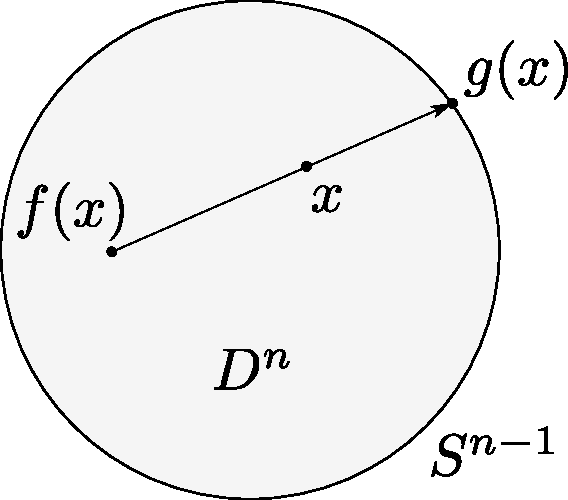
\includegraphics[width=3in]{905/Figures/10-Brouwer-FPT.pdf}
\end{center}


Our computation of the homology of a sphere also implies that there are many non-homotopic self-maps of $S^n$, for any $n\geq1$. We will distinguish them by means of the ``degree'': A map $f:S^n\to S^n$ induces an endomorphism of the infinite cyclic group $H_n(S^n)$. Any endomorphism of an infinite cyclic group is given by multiplication by an integer. This integer is well defined (independent of a choice of basis), and any integer occurs. Thus $\mathrm{End}(\ZZ)=\ZZ_\times$, the monoid of integers under multiplication. The homotopy classes of self-maps of $S^n$ also form a monoid, under composition, and: 
\begin{theorem}
Let $n\geq 1$. The degree map provides us with a surjective monoid homomorphism
\[
\mathrm{deg}:[S^n,S^n]\to \Z_\times\,.
\]
\end{theorem}
\begin{proof}
Degree is multiplicative by functoriality of homology.

Construction of a map of degree $k$: If $n=1$, this is just the winding number; an example is given by regardeing $S^1$ as unit complex numbers and sending $z$ to $z^k$. The proof that this has degree $k$ is an exercise. 

Suppose we've constructed a map $f_k:S^{n-1}\to S^{n-1}$ of degree $k$. 
Extend it to a map $\overline f_k:D^n\to D^n$ by defining 
$\overline f_k(tx)=tf_k(x)$ for $t\in[0,1]$. We may then collapse the sphere
to a point and identify the quotient with $S^n$. This gives us a new map
$g_k:S^n\to S^n$ making the diagram below commute.
	\begin{equation*}
	\xymatrix{ H_{n-1}(S^{n-1})\ar[d]^{f_{k*}} & \ar[l] H_n(D^n,S^{n-1})\ar[r]\ar[d] & H_n(S^n) \ar[d]^{g_{k*}}\\
	 H_{n-1}(S^{n-1}) & \ar[l] H_n(D^n,S^{n-1})\ar[r] & H_n(S^n)}
	\end{equation*}
The horizontal maps are isomorphisms, so $\deg g_k=k$ as well.
\end{proof}

We will see (in 18.906) that this map is in fact an isomorphism. 


\section{The Eilenberg Steenrod axioms and the locality principle}


Before we proceed to prove the excision theorem, let's review the properties of homology theory as we have developed them. They are captured by a set of axioms, due to Sammy Eilenberg and Norman Steenrod. 
\begin{definition}
A {\em homology theory} (on $\mathbf{Top}$) is:
\begin{itemize}
\item a sequence of functors $h_n:\mathbf{Top}_2\to\mathbf{Ab}$ for all $n\in\ZZ$ and
\item a sequence of natural transformations $\partial:h_n(X,A)\to h_{n-1}(A,\varnothing)$
\end{itemize}
such that:
\begin{itemize}
\item if $f_0,f_1:(X,A)\to (Y,B)$ are homotopic, then $f_{0,\ast}=f_{1,\ast}:h_n(X,A)\to h_n(Y,B)$.
\item excisions induce isomorphisms.
\item for any pair $(X,A)$, the sequence 
\begin{equation*}
\cdots\to h_{q+1}(X,A)\xrightarrow{\partial}h_q(A)\to h_q(X)\to h_q(X,A)\xrightarrow{\partial}\cdots
\end{equation*}
is exact, where we have written $h_q(X)$ for $h_q(X,\varnothing)$.
\item (the dimension axiom): $h_n(\ast)$ is nonzero only in dimension zero. 
\end{itemize}
\end{definition}
We add the following ``Milnor axiom'' to our definition. To state it,
let $I$ be a set and suppose that for each $i\in I$ we have a space $X_i$. We can form their disjoint union or {\em coproduct} $\coprod X_i$. The inclusion maps $X_i\to\coprod X_i$ induce maps $h_n(X_i)\to h_n(\coprod X_i)$, and these in turn induce a map from the direct sum, or coproduct. 
\[
\alpha:\bigoplus_i h_n(X_i)\to h_n\left(\coprod_{i\in I} X_i\right)\,.
\]
Then:
\begin{itemize}
\item The map $\alpha$ is an isomorphism for all $n$.
\end{itemize}

Ordinary singular homology satisfies these, with $h_0(\ast)=\ZZ$. We will soon add ``coefficents'' to homology, producing a homology theory whose value on a point is any prescribed abelian group. In later developments, it 
emerges that the dimension axiom is rather like the parallel postulate
in Euclidean geometry: it's ``obvious,'' but, as it turns out, the remaining
axioms accomodate extremely interesting alternatives, in which
$h_n(*)$ is nonzero for infinitely many values of $n$ (both positive and negative). 

\bigskip
Excision is a statement that homology is ``localizable.'' To make this precise, we need some definitions. 

\begin{definition}
Let $X$ be a topological space. A family $\mathscr{A}$ of subsets of $X$ is a
{\em cover} if $X$ is the union of the interiors of elements of $\mathscr{A}$. 
\end{definition}
\begin{definition}
Let ${\mathscr{A}}$ be a cover of $X$. An $n$-simplex $\sigma$ is ${\mathscr{A}}$-small if there is $A\in \mathscr{A}$ such that the image of $\sigma$ is entirely in $A$.
\end{definition}
Notice that if $\sigma:\Delta^n\to X$ is ${\mathscr{A}}$-small, then so is $d^i\sigma$; in fact, for any simplicial operator $\phi$, $\phi^*\sigma$ is again $\mathscr{A}$-small. Let's denote by $\Sin^{\mathscr{A}}_*(X)$ the graded set of ${\mathscr{A}}$-small simplices. This us a sub-simplicial set of $\Sin_*(X)$.
Applying the free abelian group functor, we get the subcomplex 
\[
S^{\mathscr{A}}_\ast(X)
\]
of $\mathscr{A}$-{\em small simplices}. Write $H^{\mathscr{A}}_*(X)$ for its
homology.
\begin{theorem}
The inclusion $S^\mathscr{A}_\ast(X)\subseteq S_\ast(X)$ is a chain homotopy equivalence, so $H^\mathscr{A}_\ast(X)\to H_\ast(X)$ is an isomorphism.
\end{theorem}
This will take a little time to prove. Let's see right now how it implies excision.

Suppose $X\supset A\supset U$ is excisive, so that 
$\overline U\subseteq\mathrm{Int}A$, or $\mathrm{Int}(X-U)\cup\mathrm{Int}A=X$.
This if we let $B=X-U$, then $\mathscr{A}=\{A,B\}$ is a cover of $X$. 
Rewriting in terms of $B$,
\[
(X-U,A-U)=(B,A\cap B)\,,
\]
so we aim to show that 
\[
S_*(B,A\cap B)\rightarrow S_*(X,A)
\]
induces an isomorphism in homology. We have the following diagram of chain complexes with exact rows:
\[
\xymatrix{
0 \ar[r] & S_*(A) \ar[d]^= \ar[r] & S^{\mathscr{A}}_*(X) \ar[d]\ar[r] &
S^{\mathscr{A}}_*(X)/S_*(A) \ar[d]\ar[r] & 0 \\
0 \ar[r] & S_*(A) \ar[r] & S_*(X) \ar[r] & S_*(X,A) \ar[r] & 0 
}\]
The middle vertical induces an isomorphism in homology by the locality principle, so the homology long exact sequences combine with the five-lemma to show that the right hand vertical is also a homology isomorphism. But 
\[
S^{\mathscr{A}}_n(X)=S_n(A)+S_n(B)\subseteq S_n(X)\,
\]
and a simple result about abelian groups provides an isomorphism
\[
\frac{S_n(B)}{S_n(A\cap B)}=
\frac{S_n(B)}{S_n(A)\cap S_n(B)}\xrightarrow{\cong}
\frac{S_n(A)+S_n(B)}{S_n(A)}
=\frac{S_n^{\mathscr{A}}(X)}{S_n(A)}\,,
\]
so excision follows.

This case of a cover with two elements leads to another expression of 
excision, known as the ``Mayer-Vietoris sequence.'' In describing it we will
use the following notation for the various inclusion.
\begin{equation*}
\xymatrix{A\cap B\ar[r]^{j_1}\ar[d]^{j_2} & A\ar[d]^{i_1}\\
B\ar[r]_{i_2} & X}
\end{equation*}
\begin{theorem}[Mayer-Vietoris] 
Assume that $\mathscr{A}=\{A,B\}$ is a cover of $X$. There are natural
maps $\partial:H_n(X)\to H_{n-1}(A\cap B)$ such that the sequence
\[
\xymatrix{
& \cdots \ar[r]^\beta & H_{n+1}(X) \ar[dll]_\partial \\
H_n(A\cap B) \ar[r]^\alpha &
H_n(A)\oplus H_n(B) \ar[r]^\beta & H_n(X) \ar[dll]_\partial \\
H_{n-1}(A\cap B) \ar[r]^\alpha & \cdots 
}\]
is exact, where 
\[ 
\alpha=\left[\begin{array}{c}j_{1*}\\-j_{2*}\end{array}\right]\,,\quad
\beta=[\,i_{1*}\quad i_{2*}\,]\,.
\]
\end{theorem}
\begin{proof}
This is the homology long exact sequence associated to the short exact sequence
of chain complexes
\[
0\to S_*(A\cap B)\xrightarrow{\alpha}S_*(A)\oplus S_*(B)\xrightarrow{\beta}
S^{\mathscr{A}}_*(X)\to0\,,
\]
combined with the locality principle.
\end{proof}

The Mayer-Vietoris theorem follows from excision as well, via
the following simple observation.
Suppose we have a map of long exact sequences
\begin{equation*}
\xymatrix{
\cdots\ar[r] & C'_{n+1} \ar[r]\ar[d] & A'_n\ar[r]\ar[d] & 
B'_n\ar[r]\ar[d]^\cong & 
C'_n\ar[r]^k\ar[d]^h & A_{n-1}\ar[r]\ar[d]^f & \cdots\\
\cdots\ar[r] & C_{n+1} \ar[r] & A_n \ar[r] & B_n \ar[r] & C_n \ar[r]^k & 
A_{n-1}\ar[r] & \cdots
}
\end{equation*}
in which every third arrow is an isomorphism as indicated.
Define a map
\[
\partial:A_n\to B_n\xleftarrow{\cong} B'_n\to C'_n\,.
\]
An easy diagram chase shows:
\begin{lemma} 
\label{lem-ladder}
The sequence 
\begin{equation*}
\cdots\longrightarrow 
C'_{n+1}\xrightarrow{\left[\begin{array}{c}h\\-k\end{array}\right]}
C_{n+1}\oplus A_n\xrightarrow{\left[\begin{array}{cc}k&f\end{array}\right]}
A_n\xrightarrow{\,\,\partial\,\,} C'_n\longrightarrow\cdots
\end{equation*}
is exact.
\end{lemma}
To get the Mayer-Vietoris sequence, let $\{A,B\}$ be a cover of $X$ 
and apply the lemma to 
\[
\xymatrix{
\cdots \ar[r] & H_n(A\cap B) \ar[d] \ar[r] & H_n(B)  \ar[d] \ar[r] &
H_n(B,A\cap B) \ar[d]^\cong \ar[r] & H_{n-1}(A\cap B) \ar[d] \ar[r] &
H_{n-1}(B) \ar[d] \ar[r] & \cdots \\
\cdots \ar[r] & H_n(A) \ar[r] & H_n(X) \ar[r] & H_n(X,A) \ar[r] & 
H_{n-1}(A) \ar[r] & H_{n-1}(X) \ar[r] & \cdots\,.
}\]


\section{Subdivision}

We will begin the proof of the locality principle today, 
and finish it in the next lecture.
The key is a process of subdivision of singular simplices. It will use the 
``cone construction'' $b*$ from Lecture 5. The cone construction 
dealt with a region $X$ 
in Euclidean space, star-shaped with respect to $b\in X$, and gave a 
chain-homotopy between the identity and the ``constant map'' on $S_*(X)$:
\[
db*+b*d=1-\eta\epsilon
\]
where $\epsilon:S_*(X)\to\ZZ$ is the augmentation and $\eta:\ZZ\to S_*(X)$
sends 1 to the constant 0-chain $c_b^0$. 

Let's see how the cone construction can be used to ``subdivide'' an ``affine 
simplex.'' An {\em affine simplex} is the convex hull of a finite set of points in Euclidean space. To make this non-degenerate, assume that the points $v_0,v_1,\ldots,v_n$, have the property that $\{v_1-v_0,\ldots,v_n-b_0\}$ is linearly independent. 
The {\em barycenter} of this simplex is the center of mass of the vertices, 
\[
b=\frac{1}{n+1}\sum{v_i}\,.
\]

Start with $n=1$. To subdivide a 1-simplex, just cut it in half. 
For the $2$-simplex, look at the subdivision of each face, and form the cone
of them with the barycenter of the 2-simplex. This gives us a decomposition of
the 2-simplex into six sub-simplices. 

\begin{center}
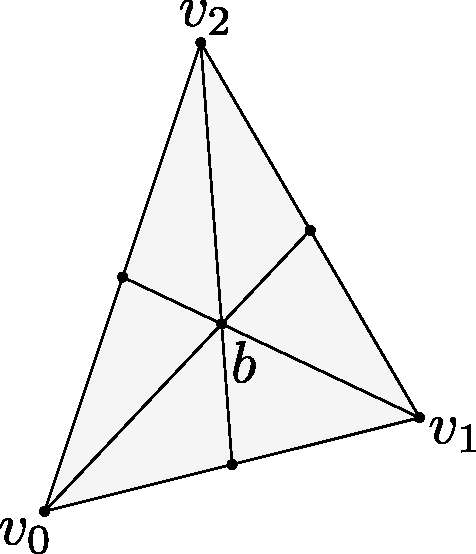
\includegraphics[width=3in]{905/Figures/12-subdivision.pdf}
\end{center}

We want to formalize this process, and extend it to singular simplices (using
naturality, of course). Define a natural transformation 
\[
\$:S_n(X)\to S_n(X)
\]
 by defining it on standard $n$-simplex, namely by specifying what $\$(\iota_n)$ is where $\iota_n:\Delta^n\rightarrow\Delta^n$ is the universal $n$-simplex, and then extending by naturality:
\[
\$(\sigma)=\sigma_\ast\$(\iota_n)\,.
\]
Here's the definition. When $n=0$, define $\$$ to be the identity; i.e., $\$\iota_0=\iota_0$. For $n>0$, define 
\[
\$\iota_n:=b_n\ast\$ d\iota_n
\]
where $b_n$ is the barycenter of $\Delta^n$. This makes a \emph{lot} of sense if you draw out a picture, and it's a very clever definition that captures the geometry we described. Here's what we'll prove.
\begin{prop}
$\$$ is a natural chain map $S_\ast(X)\to S_\ast(X)$ that is naturally chain-homotopic to the identity. 
\end{prop}

\noindent
\begin{proof}
Let's try to prove that it's a chain map. We'll use induction on $n$. It's enough to show that $d\$\iota_n=\$ d\iota_n$, because then, for any $n$-simplex $\sigma$,
$$
d\$\sigma=d\$\sigma_\ast\iota_n=\sigma_\ast d\$\iota_n=\sigma_\ast \$d\iota_n=\$ d\sigma_\ast\iota_n=\$ d\sigma\,.
$$

Dimension zero is easy:
since $S_{-1}=0$, $d\$\iota_0$ and $\$d\iota_0$ are both zero and hence equal.

For $n\geq 1$, we want to compute $d\$\iota_n$. This is:
\begin{align*}
d\$\iota_n & =d(b_n\ast \$ d\iota_n)  \\
 & = (1-\eta_b\epsilon-b_n\ast d)(\$ d\iota_n)
\end{align*}
What happens when $n=1$? Well,
$$
\eta_b\epsilon\$d\iota_1 = \eta_b\epsilon \$(c^0_1 - c^0_0)=\eta_b\epsilon(c^0_1 - c^0_0)=0\,,
$$
since $\epsilon$ takes sums of coefficients. So the $\eta_b\epsilon$ term drops out for any $n\geq1$. Let's continue, using the inductive hypothesis:
\begin{align*}
d\$\iota_n & = (1 - b_n\ast d)(\$ d\iota_n) \\
 & = \$d\iota_n - b_n\ast d\$ d\iota_n  \\
 & = \$d\iota_n - b_n\$d^2\iota_n &\\
 & = \$d\iota_n 
\end{align*}
because $d^2=0$. 

To define the chain homotopy $T$, we'll just write down a formula and not try to justify it. Making use of naturality, we just need to define $T\iota_n$. 
Here it is:
\[
T\iota_n = b_n\ast(\$\iota_n - \iota_n - Td\iota_n)\in S_{n+1}(\Delta^n) \,.
\]
Once again, we're going to check that $T$ is a chain homotopy by induction, and, again, we need to check only on the universal case.

When $n=0$, the formula gives $T\iota_0=0$, so it's true that $dT\iota_0-Td\iota_0=\$\iota_0-\iota_0$.
Now let's assume that $dTc-Tdc=\$c-c$ for every $(n-1)$-chain. Let's start by computing $dT\iota_n$:
\begin{align*}
dT\iota_n & = d_n(b_n\ast(\$\iota_n - \iota_n - Td\iota_n)) \\
& = (1-b_n\ast d)(\$\iota_n - \iota_n - Td\iota_n) \\
& = \$\iota_n-\iota_n-Td\iota_n-b_n\ast (d\$\iota_n - d\iota_n - dTd\iota_n)
\end{align*}
All we want now is that $b_n\ast(d\$\iota_n - d\iota_n - dTd\iota_n)=0$. We can do this using the inductive hypothesis, because $d\iota_n$ is in dimension $n-1$.
\begin{align*}
dTd\iota_n & = -Td(d\iota_n)+\$ d\iota_n - d\iota_n\\
& = \$d\iota_n - d\iota_n\\
& = d\$\iota_n - d\iota_n\,.
\end{align*}
This means that $d\$\iota_n-d\iota_n - dTd\iota_n=0$, so $T$ is indeed a chain homotopy. 
\end{proof}

\section{Proof of the Locality Principle}

We have constructed the subdivision operator $\$:S_*(X)\to S_*(X)$, with the
idea that it will shink chains and by iteration eventually render any chain 
$\mathscr{A}$-small. Does $\$$ succeed in making simplices smaller? Let's 
look first at the affine case. Recall that the ``diameter'' of a subset $X$ of 
a metric space is given by
\[
\mathrm{diam}(X)=\sup\{d(x,y):x,y\in X\}\,.
\]

\begin{lemma}
Let $\sigma$ be an affine $n$-simplex, and $\tau$ a simplex in $\$\sigma$.
Then $\mathrm{diam}(\tau)\leq \frac{n}{n+1}\mathrm{diam}(\sigma)$.
\end{lemma}
\begin{proof}
Suppose that the vertices of $\sigma$ are $v_0,v_1,\ldots,v_n$. Let $b$ be the 
barycenter of $\sigma$, and write the vertices of $\tau$ as $w_0=b,w_1,\ldots,w_n$. We compute
\[
|b-v_i|  =\left|\frac{v_0+\cdots+v_n-(n+1)v_i}{n+1}\right|
=\left|\frac{(v_0-v_i)+(v_1-v_i)+\cdots+(v_n-v_i)}{n+1}\right|\,.
\]
One of the terms in the numerator is zero, so we can continue: 
\[
|b-v_i| \leq \frac{n}{n+1}\max_{i,j}|v_i-v_j| 
= \frac{n}{n+1}\mathrm{diam}(\sigma)
\]
Since $w_i\in\sigma$, 
\[
|b-w_i| \leq\max_i|b-v_i| \leq \frac{n}{n+1}\mathrm{diam}(\sigma)\,.
\]
For the other cases, well, we use induction:
\[
|w_i-w_j| \leq \mathrm{diam}(\text{simplex in }\$d\sigma)
\leq \frac{n-1}{n}\mathrm{diam}(d\sigma)
\leq \frac{n}{n+1}\mathrm{diam}(\sigma)\,.
\]
\end{proof}

Now let's transfer this calculation to singular simplices in a space $X$ 
equipped with a cover $\mathscr{A}$. 
\begin{lemma}
For any singular chain $c$, some iterate of the subdivision operator sends $c$ to an $\mathscr{A}$-small chain.
\end{lemma}
\begin{proof} We may assume that $c$ is a single simplex $\sigma:\Delta^n\to X$, because in generaly you just take the largest iterate of $\$$ needed to send each simplex in $c$ to an $\mathscr{A}$-small chain.
We now encounter another of the great virtues of singular homology:
we pull $\mathscr{A}$ back to a cover of the standard simplex. 
Define an open cover $\sigma^{-1}\mathscr{A}$ of $\Delta^n$ defined by 
\[
\mathscr{U}:=\{\sigma^{-1}(\mathrm{Int}(A)):A\in\sca\}\,.
\]
The space $\Delta^n$ is a compact Hausdorff space, and so is subject to the
Lebsegue covering lemma, which we apply to the open cover 
$\{\mathrm{Int}B:B\in\sigma^{-1}\mathscr{A}\}$. 
\begin{lemma}[Lebsegue covering lemma]
Let $M$ be a compact metric space, and let $\mathscr{U}$ be an open cover. Then there is $\epsilon> 0$ such that for all $x\in M$, 
$B_\epsilon(x)\subseteq U$ for some $U\in \mathscr{U}$.
\end{lemma}
\end{proof}

To apply this, we will have to understand iterates of the subdivision operator.

\begin{lemma} For any $k\geq1$,
$\$^k\sim 1:S_\ast(X)\to S_\ast(X)$.
\end{lemma}
\begin{proof}
We construct $T_k$ such that $dT_k+T_kd=\$^k-1$. To begin, we take $T_1=T$, since $dT+Td=\$-1$. Let's apply $\$$ to this equation. We get $\$dT+\$Td=\$^2-\$$.Sum up these two equations to get 
\[
dT+Td+\$dT+\$Td = \$^2-1\,,
\] 
which simplifies to 
\[
d(\$+1)T+(\$+1)Td=\$^2-1
\]
since $\$d=d\$$.

So define $T_2=(\$+1)T$, and continuing, you see that we can define
\[
T_k=(\$^{k-1}+\$^{k-2}+\cdots+1)T\,.
\]
\end{proof}

We are now in position to prove the Locality Principle, which we recall:
\begin{theorem}
Let $\mathscr{A}$ be a cover of a space $X$. 
The inclusion $S^\mathscr{A}_\ast(X)\subseteq S_\ast(X)$ is a chain homotopy equivalence, so $H^\mathscr{A}_\ast(X)\to H_\ast(X)$ is an isomorphism.
\end{theorem}
\begin{proof}
To prove surjectivity let $c$ be an $n$-cycle in $X$. We want to find an $\sca$-small $n$-cycle that is homologous to $c$. There's only one thing to do. Pick $k$ such that $\$^k c$ is $\sca$-small. This is a cycle because because $\$^k$ is a chain map. I want to compare this new cycle with $c$. That's what the chain homotopy $T_k$ is designed for: 
\[
\$^kc-c=dT_k c+T_kdc=dT_kc
\]
since $c$ is a cycle. So $\$^kc$ and $c$ are homologous.

Now for injectivity. Suppose $c$ is a cycle in $S^\sca_n(X)$ such that $c=db$ for some $b\in S_{n+1}(X)$. We want $c$ to be a boundary of an $\sca$-small chain. Use the chain homotopy $T_k$ again: Suppose that $k$ is such that $\$^kc$ is $\sca$-small. Compute:
\[
d\$^kb-c=d(\$^k-1)b=d(dT_k+T_kd)b=dT_kc
\]
so 
\[
c=d\$^kb-dT_kc=d(\$^kb-T_kc)\,.
\]
Now, $\$^kb$ is $\sca$-small, by choice of $k$. Is $T_kc$ also $\sca$-small? I claim that it is. Why? It is enough to show that $T_k\sigma$ is $\sca$-small if $\sigma$ is. We know that $\sigma=\sigma_\ast\iota_n$. Because $\sigma$ is $\sca$-small, we know that $\sigma:\Delta^n\to X$ is the composition $i_\ast\overline{\sigma}$ where $\overline{\sigma}:\Delta^n\to A$ and $i:A\to X$ is the inclusion of some $A\in\sca$. By naturality, then, $T_k\sigma=T_ki_\ast\overline{\sigma}=i_\ast T_k\overline{\sigma}$, which certainly is $\sca$-small.
\end{proof}

This completes the proof of the Eilenberg Mac Lane axioms for singular homology. In the next chapter, we will develop a variety of practical tools, using these axioms to compute the singular homology of many spaces. 


\chapter{Computational methods}
\section{CW-complexes}

There are various ways to model geometrically interesting spaces. 
Manifolds provide one important model, well suited to analysis.  
Another model, one we have not talked 
about, is given by simplicial complexes. It's very combinatorial,
and constructing a simplicial complex model for a given space involves
making a lot of choices that are combinatorial rather than topological
in character. A more flexible model, one more closely reflecting topological
information, is given by the theory of CW-complexes. 

In building up a space as a CW-complex, we will successively ``glue'' cells
onto what has been already built. This is a general construction. 

Suppose we have a pair $(B,A)$, and a map $f:A\to X$. Define a space
$X\cup_f B$ (or $X\cup_A B$) in the diagram
\begin{equation*}
\xymatrix{A\ar[r]^f\ar@{^(->}[d] & X\ar[d]\\
B\ar[r] & X\cup_f B}
\end{equation*}
by
\[
X\cup_f B=X\sqcup B/\sim
\]
where the equivalence relation is generated by requiring that $a\sim f(a)$ 
for all $a\in A$. We say that we have ``attached $B$ to $X$ along $f$ (or 
along $A$).'' 

There are two kinds of equivalence classes in $X\cup_fB$: (1) singletons containing elements of $B-A$, and (2) $\{x\}\sqcup f^{-1}(x)$ for $x\in X$.
The topology on $X\cup_fB$ is the quotient topology, and is characterized
by a universal property: any solid-arrow commutative diagram
\begin{equation*}
\xymatrix{A\ar[r]^f\ar@{^(->}[d] & X\ar[d]^j\ar[ddr]^{\overline{j}} & \\
B\ar[r]\ar[drr]_{\overline{g}} & X\cup_f B\ar@{-->}[dr] & \\
 & & Y}
\end{equation*}
can be uniquely filled in. It's a ``push-out.''
\begin{example}
If $X=\ast$, then $\ast\cup_f B=B/A$.
\end{example}
\begin{example}
If $A=\varnothing$, then $X\cup_fB$ is the coproduct $X\sqcup B$. 
\end{example}
\begin{example}
If both, 
\[
B/\varnothing=\ast\cup_\varnothing B=\ast\sqcup B\,.
\]
For example, $\varnothing/\varnothing=\ast$. 
This is creation from nothing. We won't get into the religious ramifications.
\end{example}
\begin{example}[Attaching a cell]
A basic collection of pairs of spaces is given by the disks relative to their
boundaries: $(D^n,S^{n-1})$. (Recall that $S^{-1}=\varnothing$.) In this
context, $D^n$ is called an ``$n$-cell,'' and a map $f:S^{n-1}\to X$ allows
us to attach an $n$-cell to $X$, to form 
\begin{equation*}
\xymatrix{S^{n-1}\ar[r]^f\ar@{^(->}[d] & X\ar[d]\\
D^n\ar[r] & X\cup_f D^n}
\end{equation*}
You might want to generalize this a little bit, and attach a bunch of $n$-cells all at once:
\begin{equation*}
\xymatrix{\coprod_{\alpha\in A}S^{n-1}_\alpha\ar[r]^f\ar@{^(->}[d] & X\ar[d]\\
\coprod_{\alpha\in A}D^n_\alpha\ar[r] & X\cup_f \coprod_{\alpha\in A}D^n_\alpha}
\end{equation*}
\end{example}
What are some examples? When $n=0$, $(D^0,S^{-1})=(\ast,\varnothing)$, so 
you are just adding a discrete set to $X$:
\[
X\cup_f\coprod_{\alpha\in A}D^0=X\sqcup A
\]
More interesting: Let's attach two 1-cells to a point:
\begin{equation*}
\xymatrix{S^0\sqcup S^0\ar[r]^f\ar@{^(->}[d] & \ast\ar[d]\\
D^1\sqcup D^1\ar[r] & \ast\cup_f (D^1\sqcup D^1)}
\end{equation*}
Again there's just one choice for $f$, and 
$\ast\cup_f(D^1\sqcup D^1)$ is a figure $8$, because you start with 
two $1$-disks and identify the four boundary points together. Let me write 
$S^1\vee S^1$ for this space. We can go on and attach a single 2-cell to 
manufacture a torus. Think of the figure 8 as the perimeter of a square with opposite sides identified.

\medskip
\begin{center}
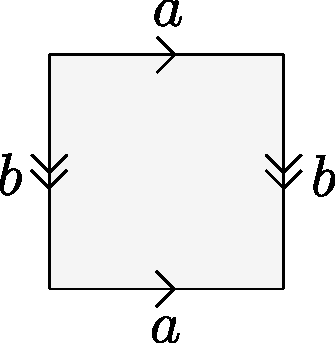
\includegraphics[width=1.75in]{905/Figures/14-torus-CW-structure.pdf}
\end{center}

The inside of the square is a 2-cell, attached to the perimeter by a map I'll denote by $aba^{-1}b^{-1}$: 
\begin{equation*}
\xymatrix{S^1\ar[r]^{aba^{-1}b^{-1}}\ar@{^(->}[d] & S^1\vee S^1\ar[d]\\
D^2\ar[r] & (S^1\vee S^1)\cup_f D^2=T^2\,.
}\end{equation*}

This example illuminates the following definition.

\begin{definition}
A \emph{CW-complex} is a space $X$ equipped with a sequence of subspaces 
\[
\varnothing=\Sk_{-1}X\subseteq\Sk_0X\subseteq\Sk_1X\subseteq\cdots\subseteq X
\]
such that 
\begin{itemize}
\item $X$ is the union of the $\Sk_nX$'s, and 
\item for all $n$, there is a pushout diagram like this:
\begin{equation*}
\xymatrix{\coprod_{\alpha\in A_n}S^{n-1}_\alpha\ar[r]^-{f_n}\ar@{^(->}[d] 
& \Sk_{n-1}X\ar[d]\\
\coprod_{\alpha\in A_n}D^n_\alpha\ar[r]^-{g_n} & \Sk_nX}\,.
\end{equation*}
\end{itemize}
\end{definition}
The subspace $\Sk_nX$ is the $n$-{\em skeleton} of $X$. 
Sometimes it's convenent to use the alternate notation $X_n$ 
for the $n$-skeleton.
The first condition is intended topologically, so that a subset of $X$ is open if and only if its intersection with each $\Sk_nX$ is open; or, equivalently, a map $f:X\to Y$ is continuous if and only if its restriction to each $\Sk_nX$ is continuous. The maps $f_n$ are the {\em attaching maps} and the maps $g_n$ are {\em characteristic maps}. 

\begin{example}
We just constructed the torus as a CW complex with $\Sk_0T^2=\ast$, $\Sk_1T^2=S^1\vee S^1$, and $\Sk_2T^2=T^2$.
\end{example}
\begin{definition}
A CW-complex is \emph{finite-dimensional} if $\Sk_nX=X$ for some $n$;
of \emph{finite type} if each $A_n$ is finite, i.e., finitely many cell in each dimension; and \emph{finite} if it's finite-dimensional and of finite type.
\end{definition}
The {\em dimension} of a CW complex is the largest $n$ for which there are 
$n$-cells. This is not obviously a topological invariant, but, have no fear,
it turns out that it is.

In ``CW,'' the ``C'' is for cell, and the ``W'' is for weak, because of the topology on a CW-complex. This definition is due to J. H. C. Whitehead. Here are a couple of important facts about them. 
\begin{theorem}
Any CW-complex is Hausdorff, and it's compact if and only if it's finite. \\
Any compact smooth manifold admits a CW structure.
\end{theorem}
\begin{proof} See \cite{bredon} Prop. IV.8.1, \cite{hatcher} Prop. A.3.
\end{proof}


\section{CW-complexes II}

We have a few more general things to say about CW complexes. 

Suppose $X$ is a CW complex, with skeleton filtration 
$\varnothing=X_{-1}\subseteq X_0\subseteq X_1\subseteq\cdots\subseteq X$ and 
cell structure
\begin{equation*}
\xymatrix{\coprod_{\alpha\in A_n}S^{n-1}_\alpha\ar[r]^{f_n}\ar@{^(->}[d] & X_{n-1}\ar[d]\\
\coprod_{\alpha\in A_n}D^n_\alpha\ar[r]^{g_n} & X_{n}}\,.
\end{equation*}
In each case, the boundary of a cell gets identified with part of the previous skeleton, but the ``interior''
\[
\mathrm{Int}D^n=\{x\in D^n:|x|<1\}
\]
does not. (Note that $\mathrm{Int}D^0=D^0$.) Thus as sets -- ignoring
the topology -- 
\[
X=\coprod_{n\geq 0}\coprod_{\alpha\in A_n}\mathrm{Int}(D^n_\alpha)\,.
\]
The subsets $\mathrm{Int}D^n_\alpha$ are called ``open $n$-cells,'' 
despite the fact that they not generally open in the topology on $X$,
and (except when $n=0$) they are not homeomorphic to compact disks.

\begin{definition}
Let $X$ be a CW-complex with a cell structure $\{g_\alpha:D^n_\alpha\to X_n|\alpha\in A_n\}$. A {\em subcomplex} is a subspace $Y\subseteq X$ such that for all $n$, there is a subset $B_n$ of $A_n$ such that $Y_n=Y\cap X_n$ provides $Y$ with a CW-structure with characteristic maps $\{g_\beta|\beta\in B_n\}$.
\end{definition}
\begin{example}
$\Sk_nX\subseteq X$ is a subcomplex.
\end{example}
\begin{prop}[\cite{bredon}, p. 196]
Let $X$ be a CW-complex with a chosen cell structure. Any compact subspace
of $X$ lies in some finite subcomplex. 
\end{prop}
\begin{remark}
For fixed cell structures, unions and intersections of subcomplexes are subcomplexes.
\end{remark}

The $n$-sphere $S^n$ (for $n>0$) 
admits a very simple CW structure:
Let $\ast=\mathrm{Sk}_0(S^n)=\mathrm{Sk}_1(S^n)=\cdots=\mathrm{Sk}_{n-1}(S^n)$,
and attach an $n$-cell using the unique map $S^{n-1}\to\ast$. This is a 
minimal CW structure -- you need at least two cells to build $S^n$. 

This is great -- much simpler than the simplest construction of $S^n$ as 
a simplicial complex -- but it is not ideal for all applications.  
Here's another CW-structure on $S^n$. Regard $S^n\subseteq\RR^{n+1}$, 
filter the Euclidean space by leading subspaces
\[
\RR^k=\langle e_1,\ldots,e_k\rangle\,.
\]
and define 
\[
\mathrm{Sk}_kS^n=S^n\cap\RR^{k+1}=S^k\,.
\]

\fbox{picture needed}

Now there are two $k$-cells for each $k$ with $0\leq k\leq n$, given by the
two hemispheres of $S^k$. For each $k$ there are two characteristic maps,
\[
u,\ell:D^k\to S^k 
\]
defining the upper and lower hemispheres:
\[
u(x)=(x,\sqrt{1-|x|^2})\,,\quad\ell(x)=(x,-\sqrt{1-|x|^2})\,.
\]
Note that if $|x|=1$ then $|u(x)|=|\ell(x)|=1$, so each characteristic map
restricts on the boundary to a map to $S^{k-1}$, and serves as an attaching 
map. This cell structure has the advantage that $S^{n-1}$ is a subcomplex 
of $S^n$. 

The case $n=\infty$ is allowed here. Then $\RR^\infty$ denotes the countably
infinite dimensional inner product space that is the topological union of the
leading subspaces $\RR^n$. The CW-complex $S^\infty$ is of finite type but
not finite dimensional. It has the following interesting property. We know that
$S^n$ is not contractible (because the identity map and a constant map have 
different behavior in homology), but: 
\begin{prop}
$S^\infty$ is contractible.
\end{prop}
\begin{proof}
This is an example of a ``swindle,'' making use of infinite dimensionality. 
Let $T:\RR^\infty\to\RR^\infty$ send $(x_1,x_2,\ldots)$ to 
$(0,x_1,x_2,\ldots)$. This sends $S^\infty$ to itself. The location of the 
leading nonzero entry is different for $x$ and $Tx$, so the line segment 
joining $x$ to $Tx$ doesn't pass through the origin. Therefore 
\[
x\mapsto\frac{tx+(1-t)Tx}{|tx+(1-t)Tx|} 
\]
provides a homotopy $1\simeq T$. On the other hand, $T$ is homotopic to the 
constant map with value $(1,0,0,\ldots)$, again by an affine homotopy. 
\end{proof}

This ``inefficient'' CW structure on $S^n$ has a second advantage: it's
``equivariant'' with respect to the antipodal involution. This provides us
with a CW structure on the orbit space for this action. 

Recall that $\mathbf{RP}^k=S^k/\sim$ where $x\sim -x$. The quotient map
$S^k\to\mathbf{RP}^k$ is a double cover, identifying upper and lower 
hemispheres. The inclusion of one sphere in the next is compatible with
this equivalence relation, and gives us ``linear'' embeddings 
$\mathbf{RP}^{k-1}\subseteq\mathbf{RP}^k$. 
This suggests that
\[
\varnothing\subseteq\mathbf{RP}^0\subseteq\mathbf{RP}^1\subseteq\cdots
\subseteq\mathbf{RP}^n
\]
might serve as a CW filtration. Indeed, for each $k$,
\begin{equation*}
\xymatrix{
S^{k-1} \ar[r] \ar[d] & D^k \ar[d]^u \\
\mathbf{RP}^{k-1} \ar[r] & \mathbf{RP}^k 
}\end{equation*}
is a pushout: A line in $\RR^{k+1}$ either lies in $\RR^k$ or is determined 
by a unique point in the upper hemisphere of $S^k$.




\section{Homology of CW-complexes}


The skeleton filtration of a CW complex leads to a long exact sequence in 
homology, showing that the relative homology $H_*(X_k,X_{k-1})$ controls how
the homology changes when you  pass from $X_{k-1}$ to $X_k$. What is this
relative homology? If we pick a set of attaching maps, we get the following 
diagram.
\begin{equation*}
\xymatrix{\coprod_{\alpha}S^{k-1}\ar@{^(->}[r]\ar[d]^f & \coprod_{\alpha}D^k_\alpha\ar[r]\ar[d] & \bigvee_{\alpha}S^k_\alpha\ar@{-->}[d]\\
X_{k-1}\ar@{^(->}[r] & X_k\cup_f B\ar[r] & X_k/X_{k-1}}
\end{equation*}
where $\bigvee$ is the wedge sum (disjoint union with all basepoints identified): $\bigvee_{\alpha}S^k_\alpha$ is a bouquet of spheres. The dotted
map exists and is easily seen to be a homeomorphism. 

Luckily, the inclusion $X_{k-1}\subseteq X_k$ satisfies what's needed to conclude that 
\[
H_q(X_k,X_{k-1})\to H_q(X_k/X_{k-1},\ast)
\]
is an isomorphism. After all, $X_{k-1}$ is a deformation retract of the space 
you get from $X_k$ by deleting the center of each $k$-cell. 

We know $ H_q(X_k/X_{k-1},\ast)$ very well:
\[
H_q(\bigvee_{\alpha\in A_k}S^k_\alpha,*)\cong\begin{cases}\Z[A_k] & q=k \\ 0 & q\neq k\end{cases}\,.
\]
Lesson: The relative homology $ H_k(X_k,X_{k-1})$ keeps track of the $k$-cells of $X$.
\begin{definition}
The group of {\em cellular $n$-chains} in a CW complex $X$ is
\[
C_k(X):= H_k(X_k,X_{k-1})=\Z[A_k]\,.
\]
\end{definition}
If we put the fact that $H_q(X_k,X_{k-1})=0$ for $q\neq k,k+1$
into the homology long exact sequence of the pair, we find first that
\[
H_q(X_{k-1})\xrightarrow{\cong}H_q(X_k)\quad\hbox{for}\quad q\neq k,k-1\,,
\]
and then that there is a short exact sequence
\[
0\to H_k(X_k)\to C_k(X) \to H_{k-1}(X_{k-1}) \to 0\,.
\]

So if we fix a dimension $q$, and watch how $H_q$ varies as we move through the
skelata of $X$, we find the following picture. Say $q>0$. Since $X_0$ is
discrete, $H_q(X_0)=0$. Then $H_q(X_k)$ continues to be 0 till you get up to
$X_q$. $H_q(X_q)$ is a subgroup of the free abelian group $C_q(X)$ and hence is
free abelian. Relations may get introduced into it when we pass to $X_{q+1}$; 
but thereafter all the maps 
\[
H_q(X_{q+1})\to H_q(X_{q+2})\to\cdots
\]
are isomorphisms. All the $q$-dimensional homology of $X$ is created on $X_q$,
and all the relations in $H_q(X)$ occur by $X_{q+1}$. 

This stable value of $H_q(X_k)$ maps isomorphically to $H_q(X)$, 
even if $X$ is infinite 
dimensional. This is because the union of the images of any finite set of 
singular simplices in $X$ is compact and so lies in a finite subcomplex and in
particular lies in a finite skeleton. So any chain in $X$ is the image of 
a chain in some skeleton. Since $H_q(X_k)\xrightarrow{\cong}H_q(X_{k+1})$ for 
$k>q$, we find that $H_q(X_q)\to H_q(X)$ is surjective. Similarly, 
if $c\in S_q(X_k)$ is a boundary in $X$, then it's a boundary in $X_\ell$ 
for some $\ell\geq k$. This shows that the map $H_q(X_{q+1})\to H_q(X)$ is
injective. We summarize:
\begin{prop} 
Let $k,q\geq 0$. Then 
\[
H_q(X_k)=0\quad\hbox{\em for}\,\,k<q
\]
and
\[
H_q(X_k)\xrightarrow{\cong}H_q(X)\quad\hbox{\em for}\,\,k>q\,.
\]
In particular, $H_q(X)=0$ if $q$ exceeds the dimension of $X$. 
\end{prop}

We have defined the cellular $n$-chains of a CW complex $X$,
\[
C_n(X)=H_n(X_n,X_{n-1})\,,
\]
and found that it is the free abelian group on the set of $n$ cells. 
We claim that these abelian groups are related to each other; they form 
the groups in a chain complex. 

What should the boundary of an $n$-cell be? It's represented by 
a characteristic map $D^n\to X_n$ whose boundary is the attaching map 
$\alpha:S^{n-1}\to X_{n-1}$.
This is a lot of information, and hard to interpret because $X_{n-1}$ is itself
potentially a complicated space. But things get much simpler if I pinch out
$X_{n-2}$. This suggests defining 
\[
d:C_n(X)=H_n(X_n,X_{n-1})\xrightarrow{\partial} H_{n-1}(X_n)\rightarrow 
H_{n-1}(X_{n-1},X_{n-2})=C_{n-1}(X)\,.
\]

The fact that $d^2=0$ is embedded in the following large diagram, in which 
the two columns and the central row are exact. 
\begin{equation*}
\xymatrix{C_{n+1}(X)= H_{n+1}(X_{n+1},X_n)\ar[d]^{\partial_n}\ar[dr]^d & & 0= H_{n-1}(X_{n-2})\ar[d]\\
 H_n(X_n)\ar@{>->}[r]^{j_n}\ar[d] & C_n(X)= H_n(X_n,X_{n-1})\ar[r]^{\partial_{n-1}}\ar[dr]^d & H_{n-1}(X_{n-1})\ar[d]^{j_{n-1}}\\
 H_n(X_{n+1})\ar[d] & & C_{n-1}(X)= H_{n-1}(X_{n-1},X_{n-2})\\
0 = H_n(X_{n+1},X_n)}
\end{equation*}
Now, $\partial_{n-1}\circ j_n=0$. So the composite of the diagonals is zero, i.e., $d^2=0$, and we have a chain complex! This is the ``cellular chain complex'' of $X$. 

We should compute the homology of this chain complex, $ H_n(C_\ast(X))=\ker d/\img d$. Now
\[
\ker d=\ker (j_{n-1}\circ\partial_{n-1})\,.
\]
But $j_{n-1}$ is injective, so 
\[
\ker d=\ker\partial_{n-1}=\img j_n=H_n(X_n)\,.
\]

On the other hand 
\[
\img d=j_n(\img\partial_n)=\img\partial_n\subseteq H_n(X_n)\,.
\]
So 
\[
H_n(C_*(X))=H_n(X_n)/\img\partial_n=H_n(X_{n+1})
\]
by exactness of the left column; but as we know this is exactly $H_n(X)$!
We have proven the following result.
\begin{theorem} \label{thm-cw-homology}
For a CW complex $X$, there is an isomorpphism
\[
H_\ast(C_\ast(X))\cong H_\ast(X)
\]
natural with respect to filtration-preserving maps between CW complexes.
\end{theorem}
This has an immediate and surprisingly useful corollary.
\begin{corollary}
Suppose that the CW complex $X$ has only even cells -- that is, 
$X_{2k}\hookrightarrow X_{2k+1}$ is an isomorphism for all $k$.
Then 
\[
H_*(X)\cong C_*(X)\,.
\]
That is, $H_n(X)=0$ for $n$ odd, is free abelian for all $n$, 
and the rank of $H_n(X)$ for $n$ even is the number of $n$-cells. 
\end{corollary}
\begin{example}
Complex projective space $\CP^n$ has a CW structure in which 
\[
\Sk_{2k}\CP^n=\Sk_{2k+1}\CP^n=\CP^k\,.
\] 
The attaching $S^{2k-1}\to\CP^k$
sends $v\in S^{2k-1}\subseteq\CC^n$ to the complex line through $v$. So 
\[
H_k(\CP^n)=\begin{cases}\Z & \hbox{for}\,\,0\leq k\leq 2n,\, k\,\,\hbox{even}\\
0 & \hbox{otherwise}
\,.\end{cases}
\]
\end{example}

Finally, notice that in our proof of Theorem \ref{thm-cw-homology} we used only properties contained in the Eilenberg-Steenrod axioms. As a result,
any construction of a homology theory satisfying the Eilenberg-Steenrod axioms gives you the same values on CW complexes as singular homology. 

\section{Real projective space}


Let's try to compute $H_\ast(\mathbf{RP}^n)$. This computation will invoke a 
second way to think of the cellular chain group $C_n(X)$. Each cell has a 
characteristic map $D^n\to X_n$, and we have the diagram
\[
\xymatrix{
\coprod(D^n,S^{n-1}) \ar[r] \ar[dr] & (X_n,X_{n-1}) \ar[d] \\
& (\bigvee S^n,\ast).
}\]
We've shown that the vertical map induces an isomorphism in homology, and
the diagonal does as well. (For example, $\coprod D^n$ has a CW structure 
in which the $(n-1)$-skeleton is $\coprod S^{n-1}$.) So 
\[
H_n(\textstyle{\coprod}(D^n,S^{n-1}))\xrightarrow{\cong}C_n(X).
\]
 
We have a CW structure on $\RP^n$ with $\mathrm{Sk}_k(\RP^n)=\RP^k$;
there is one $k$-cell -- which we'll denote by $e_k$ -- for each $k$ between $0$ and $n$. So the cellular chain complex looks like this:
\begin{equation*}
\xymatrix{0  & C_0(\mathbf{RP}^n)\ar@{=}[d]\ar[l] & C_1(\mathbf{RP}^n)\ar@{=}[d]\ar[l] & \cdots\ar[l] & C_n(\mathbf{RP}^n)\ar@{=}[d]\ar[l] & 0 \ar[l]\\
0 & \Z\langle e^0\rangle \ar[l] & \Z\langle e^1\rangle\ar[l]_{d=0} & \cdots\ar[l] & \Z\langle e^n\rangle\ar[l] & 0 \ar[l] }
\end{equation*}
The first differential is zero because we know what $ H_0(\mathbf{RP}^n)$ is (it's $\Z$!). The differential in the cellular chain complex is given by the top
row in the following commutative diagram.
\begin{equation*}
\xymatrix{C_n= H_n(\mathbf{RP}^n,\mathbf{RP}^{n-1})\ar[r]^\partial & 
H_{n-1}(\mathbf{RP}^{n-1}) \ar[r] \ar[dr] & 
H_{n-1}(\mathbf{RP}^{n-1},\mathbf{RP}^{n-2})=C_{n-1} \ar[d]_{\cong} \\
H_n(D^n,S^{n-1}) \ar[u]_\cong \ar[r]^\partial_\cong & 
H_{n-1}(S^{n-1}) \ar[u]_{\pi_*} \ar[r] & H_{n-1}(D^{n-1}/S^{n-2},\ast)\,.
}
\end{equation*}
The map $\pi:S^{n-1}\to\RP^{n-1}$ is the attaching map of the top cell of $RP^n$; that is, the double cover. The diagonal composite pinches the subspace 
$\RP^{n-2}$ to a point. The composite map $S^{n-1}\to D^{n-1}/S^{n-2}$ 
factors as follows: 
\begin{equation*}
\xymatrix{S^{n-1}\ar[r]^{\text{double cover}}\ar[dr] & \mathbf{RP}^{n-1}\ar[r]^{\text{pinch}} & D^{n-1}/S^{n-2}\cong S^{n-1}\\
 & S^{n-1}/S^{n-2}=S^{n-1}\vee S^{n-1}\ar[ur]}
\end{equation*}
One of the maps $S^{n-1}\to S^{n-1}$ from the wedge is the identity, and the other map is the antipodal map $\alpha:S^{n-1}\to S^{n-1}$. Write $\sigma$ for a generator of $ H_{n-1}(S^{n-1})$. Then in $H_{n-1}$ we have $\sigma\mapsto (\sigma,\sigma)\mapsto \sigma+\alpha_\ast\sigma$. So we need to know the degree of the antipodal map on $S^{n-1}$. The antipodal map reverses all $n$ coordinates in $\RR^n$. Each reversal is a reflection, and acts on $S^{n-1}$ by a map of degree $-1$. So 
\[
\deg\alpha=(-1)^n\,.
\]
Therefore the cellular complex of $\RP^n$ is as follows: 
\begin{equation*}
\xymatrix@R=8pt{
\hbox{dim} & -1 & 0 & 1 & \cdots & n & n+1 & \cdots \\
& 0 & \Z\ar[l]_0 & \Z\ar[l]_2 & \cdots\ar[l]_0 & \Z\ar[l]_{2\text{ or }0} & 0\ar[l] & \cdots\ar[l]}
\end{equation*}
The homology is then easy to read off.
\begin{prop}
The homology of real projective space is as follows.
\begin{equation*}
 H_k(\RP^n)=\begin{cases}
\Z & k=0\\
\Z & k=n\text{ odd}\\
\Z/2\Z & k\text{ odd, }0<k<n\\
0 & \text{otherwise}\,.
\end{cases}
\end{equation*}
\end{prop}
Here's a table. Missing entries are $0$.
\[
\xymatrix@R=8pt{
\text{dim} & 0 & 1 & 2 & 3 & 4 & 5 & \cdots \\
\RP^0 & \ZZ \\
\RP^1 & \ZZ & \ZZ \\
\RP^2 & \ZZ & \ZZ/2 \\
\RP^3 & \ZZ & \ZZ/2 & 0 & \ZZ \\
\RP^4 & \ZZ & \ZZ/2 & 0 & \ZZ/2 \\
\RP^5 & \ZZ & \ZZ/2 & 0 & \ZZ/2 & 0 & \ZZ 
\vdots & \vdots & \vdots & \vdots & \vdots & \vdots & \vdots
}\]
Summary: In real projective space, 
odd cells create new generators; even cells (except for the zero-cell) create
torsion in the previous dimension. 

This example illustrates the significance of cellular homology, and, therefore,
of singular homology. A CW structure involves attaching maps 
\[
\textstyle{\coprod}S^{n-1}\to\Sk_{n-1} X\,.
\]
Knowing these, up to homotopy, determines the full homotopy type of the CW 
complex. Homology does not record all this information. Instead, it records 
only information about the composite obtained by pinching out $\Sk_{n-2}X$.
\[
\xymatrix{ 
\coprod_{a\in A_n} S^{n-1}_a \ar[r] \ar[dr] & \Sk_{n-1} X \ar[d] \\
& \bigvee_{b\in A_{n-1}} S^{n-1}_b\,.
}\]
In $H_{n-1}$, this can be identified with a map
\[
\partial:\Z[A_n]\to\Z[A_{n-1}]
\]
that is none other than the differential in the cellular chain complex.

The moral: homology picks off only the ``first order'' structure of a CW 
complex. 

On the other hand, we'll see in the next lecture that it does a very good job
of that. 



\section{Euler characteristic and homology approximation}


\begin{theorem} Let $X$ be a finite CW-complex with $a_n$ $n$-cells. Then 
\[
\chi(X)=\sum^\infty_{k=0}(-1)^k a_k
\]
depends only on the homotopy type of $X$; it is independent of the choice of
CW structure. 
\end{theorem}
This integer $\chi(X)$ is called the {\em Euler characteristic} of $X$. We will prove this theorem by showing that $\chi(X)$ equals a number computed from the homology groups of $X$, which are themselves homotopy invariants. 

We'll need a little bit of information about the structure of finitely generated abelian groups.

Let $A$ be an abelian group. The set of {\em torsion} elements of $A$,
\[
\mathrm{Tors}(A)=\{a\in A:na=0\,\,\text{for some}\,\,n\neq0\}\,,
\]
is a subgroup of $A$. A group is \emph{torsion free}
if $\mathrm{Tors}(A)=0$. For any $A$ the quotient group 
$A/\mathrm{Tors}(A)$ is torsion free. 

For a general abelian group, that's about all you can say. But now assume $A$ is finitely generated. Then $\mathrm{Tors}(A)$ is a finite abelian group and
$A/\mathrm{Tors}(A)$ is a finitely generated free abelian group, isomorphic to $\Z^r$ for some integer $r$ called the \emph{rank} of $A$. Pick elements of
$A$ that map to a set of generators of $A/\mathrm{Tors}(A)$, and use them
to define a map $A/\mathrm{Tors}A\to A$ splitting the projection map. This shows that if $A$ is finitely generated then
\[
A\cong\mathrm{Tors}(A)\oplus\Z^r\,.
\]

A finite abelian group $A$ is necessarily of the form 
\[
\Z/n_1\oplus\Z/n_2\oplus\cdots\oplus\Z/n_t\,\,\hbox{where}\,\,
n_1|n_2|\cdots|n_t\,.
\]
The $n_i$ are the ``torsion coefficients'' of $A$. 
They are well defined natural numbers.

\begin{lemma} Let $0\to A\to B\to C\to 0$ be a short exact sequence of finitely
generated abelian groups. Then
\[
\mathrm{rank}\,A-\mathrm{rank}\,B+\mathrm{rank}\,C=0\,.
\]
\end{lemma}

\begin{theorem} Let $X$ be a finite CW complex. Then
\[
\chi(X)=\sum_k(-1)^k\mathrm{rank}\,H_k(X)\,.
\]
\end{theorem}

\begin{proof}
Pick a CW-structure with, say, $a_k$ $k$-cells for each $k$. We have the 
cellular chain complex $C_*$. Write $H_*,Z_*$, and $B_*$ for the homology,
the cycles, and the boundaries, in this chain complex. From the definitions, 
we have two families of short exact sequences: 
\[
0\to Z_k\to C_k\to B_{k-1}\to 0
\]
and
\[
0\to B_k\to Z_k\to H_k\to 0\,.
\]
Let's use them and facts about rank rewrite the alternating sum:
\begin{align*}
\sum_k (-1)^ka_k & = \sum_k(-1)^k\mathrm{rank}(C_k)\\
& = \sum_k(-1)^k(\mathrm{rank}\,(Z_k)+\mathrm{rank}\,(B_{k-1}))\\
& = \sum_k(-1)^k(\mathrm{rank}\,(B_k)+\mathrm{rank}\,(H_k)+
\mathrm{rank}\,(B_{k-1}))
\end{align*}
The terms $\mathrm{rank}\,B_k\,+\,\mathrm{rank}\,B_{k-1}$ cancel because it's an alternating sum. This leaves $\sum_k(-1)^k\mathrm{rank}\,H_k$. But 
$H_k\cong H_k^\text{sing}(X)$.
\end{proof}

In the early part of the 20th century, ``homology groups'' were not discussed. 
It was Emmy Noether who first described things that way. Instead, 
people worked mainly with the sequence of ranks, 
\[
\beta_k=\mathrm{rank}\,H_k(X)\,,
\]
which are known (following Poincar\'e) as the {\em Betti numbers} of $X$.

Given a CW-complex $X$ of finite type, can we give a lower bound on the number of $k$-cells in terms of the homology of $X$? Let's see. $H_k(X)$ is finitely generated because $C_k(X)\hookleftarrow Z_k(X)\twoheadrightarrow H_k(X)$. Thus 
\[
H_k(X)=\bigoplus^{t(k)}_{i=1}\Z/n_i(k)\Z\oplus \Z^{r(k)}
\]
where the $n_1(k)|\cdots|n_{t(k)}(k)$ are the torsion coefficients of $H_k(X)$ 
and $r(k)$ is the rank.

The minimal chain complex with $H_k=\Z^r$ and $H_q=0$ for $q\neq k$ is just the chain complex with $0$ everywhere except for $\Z^r$ in the $k$th degree. The minimal chain complex {\em of free abelian groups} with $ H_k=\Z/n\Z$ and $ H_q=0$ for $q\neq k$ is the chain complex with $0$ everywhere except in dimensions $k+1$ and $k$, where we have $\Z\xrightarrow{n}\Z$ 
These small complexes are called {\em elementary chain complexes}.

This implies that a lower bound on the number of $k$-cells is 
\[
r(k)+t(k)+t(k-1)\,.
\]
The first two terms give generators for $H_k$, and the last gives relations
for $H_{k-1}$.

These elementary chain complexes can be realized as the reduced cellular chains of CW complexes (at least if $k>0$). A wedge of $r$ copies of $S^k$ has a CW structure with one $0$-cell and $r$ $k$-cells, so its cellular chain complex 
has  $\Z^r$ in dimension $k$ and 0 in other positive dimensions.
To construct a CW complex with cellular chain complex given by $\Z\xrightarrow{n}\Z$ in dimensions $k+1$ and $k$ and $0$ in other positive dimensions, 
start with $S^k$ as $k$-skeleton and attach a $k+1$-cell 
by a map of degree $n$. For example, when $k=1$ and $n=2$, you have $\RP^2$. 
These CW complexes are called ``Moore spaces.'' 

This maximally efficient construction of a CW complex in a homotopy type
can in fact be achieved, at least in the simply connected case:

\begin{theorem}[Wall, \cite{wall}]
Let $X$ be a simply connected CW-complex of finite type. Then there exists a CW complex $Y$ with $r(k)+t(k)+t(k-1)$ $k$-cells, for all $k$, and a homotopy equivalence $Y\to X$.
\end{theorem}

We will prove this theorem in 18.906.

The construction of Moore spaces can be generalized:
\begin{prop} For any graded abelian group $A_*$ with $A_k=0$ for $k\leq0$, 
there exists a CW complex $X$ with $\widetilde H_*(X)=A_*$.
\end{prop}
\begin{proof}
Let $A$ be any abelian group. Pick generators for $A$. 
They determine a surjection
from a free abelian group $F_0$. The kernel $F_1$ of that surjection is free,
being a subgroup of a free abelian group. Write $G_0$ for minimal set of
generators of $F_0$, and $G_1$ for a minimal set of generators for $F_1$.

Let $k\geq1$. Define $X_k$ to be the wedge of $|G_0|$ copies of $S^k$,
so $H_k(X_k)=\Z G_0$. Now define an attaching map 
\[
\alpha:\coprod_{b\in G_1} S^k_b\to X_k
\]
by specifying it on each summand $S^k_b$. The generator 
$b\in G_1$ is given by a linear combination of the generators
of $F_0$, say 
\[
b=\sum_{i=1}^s n_ia_i\,.
\]
We want to mimic this in topology. To do this, first
map $S^k\to\bigvee^s S^k$ by pinching $(s-1)$ tangent circles to points. 
In homology, this map takes a generator of $H_k(S^k)$ to the sum of the
generators of the $k$-dimensional homology of the various spheres in the
bouquet.
Map the $i$th sphere in the wedge to $S^k_{a_i}\subseteq X_k$ by a map of
degree $n_i$. The map on the summand $S^k_b$ is then the composite of these 
two maps,
\[
S^k_b\to\bigvee_{i=1}^s S^k\to\bigvee_a S^k_a\,.
\]
Altogether, we get a map $\alpha$ that realizes $F_1\to F_0$ in $H_k$.
So using it as an attaching map produces a CW complex $X$ with 
$\widetilde H_q(X)=A$ for $q=k$ and 0 otherwise. Write $M(A,k)$ for 
a CW complex produced in this way.

Finally, given a graded abelian group $A_*$, form the wedge over $k$ of the
spaces $M(A_k,k)$. 
\end{proof}

Such a space $M(A,k)$, with $\widetilde H_q(M(A,k))=A$ for $q=k$ and 0 
otherwise, is called a {\em Moore space of type} $(A,k)$ \cite{moore}. 
The notation is a bit deceptive, since $M(A,k)$ cannot be made into a functor
$\mathbf{Ab}\to\mathrm{Ho}\mathbf{Top}$.



\section{Coefficients}

Abelian groups can be quite complicated, even finitely generated ones. Vector spaces over a field are so much simpler! A vector space is determined up to isomorphism by a single cardinality, its dimension. Wouldn't it be great to have a version of homology that took values in the category of vector spaces over a field? 

We can do this, and more. Let $R$ be any commutative ring at all.
Instead of forming the free abelian group on $\Sin_*(X)$, we could just as 
form the free $R$-module:
\[
S_*(X;R)=R\Sin_*(X)
\]
This gives, first, a simplicial object in the category of $R$-modules.
Forming the alternating sum of the face maps produces a chain complex 
{\em of $R$-modules}: $S_n(X;R)$ is an $R$-module for each $n$, and 
$d:S_n(X;R)\to S_{n-1}(X;R)$ is an $R$-module homomorphism. The homology
groups are then again $R$-modules:
\[
H_n(X;R)=\frac{\ker(d:S_n(X;R)\to S_{n-1}(X;R))}
{\img(d:S_{n+1}(X;R)\to S_n(X;R))}\,.
\]

This is the {\em singular homology of $X$ with coefficients in the commutative 
ring $R$}. It satisfies all the Eilenberg-Steenrod axioms, but 
\[
H_n(\ast;R)=
\begin{cases}R\,\,&\hbox{for}\quad n=0\\0\,\,&\hbox{otherwise}\,.\end{cases}
\]
We could actually have replaced the ring $R$ by any abelian group here, 
but this will become much clearer after we have the tensor product as a tool.

The coefficient rings that are most important in algebraic topology are 
simple ones: the integers and the prime fields $\FF_p$ and $\QQ$; 
typically, a PID.

As an experiment, let's compute $ H_\ast(\RP^n;R)$ for various rings $R$.
Let's start with $R=\FF_2$, the field with 2 elements. This is a favorite
among algebraic topologists, because using it for coefficients eliminates 
all sign issues. The cellular chain complex has $S_k(\RP^n;\FF_2)=\FF_2$ for 
$0\leq k\leq n$, and the differential alternates between multiplication by 
2 and by 0. But in $\FF_2$, $2=0$: so $d=0$, and the cellular chains
coincide with the homology:
\[
H_k(\RP^n;\FF_2)=
\begin{cases}\FF_2\,&\hbox{for}\quad 0\leq k\leq n\\0\,\,&\hbox{otherwise}\,.
\end{cases}
\]

On the other hand, suppose that $R$ is a ring in which $2$ is invertible.
The universal case is $\Z[1/2]$, but any subring of the rationals containing
$1/2$ would do just as well, as would $\FF_p$ for $p$ odd. 
Now the cellular chain complex (in dimensions 0 through $n$)
looks like
\[
R\xleftarrow{0}R\xleftarrow{\cong}R\xleftarrow{0}R
\xleftarrow{\cong}\cdots\xleftarrow{\cong}R
\]
for $n$ even, and
\[
R\xleftarrow{0}R\xleftarrow{\cong}R\xleftarrow{0}R
\xleftarrow{\cong}\cdots\xleftarrow{0}R
\]
for $n$ odd. Therefore
\[
H_k(\RP^n;R)=
\begin{cases}R\,&\hbox{for}\quad k=0\\0\,&\,\hbox{otherwise}\end{cases}
\]
for $n$ even, and 
\[
H_k(\RP^n;R)=
\begin{cases}R\,&\hbox{for}\quad k=0\\
R\,&\,\hbox{for}\quad k=n\\
0\,&\,\hbox{otherwise}\,.
\end{cases}
\]
You get a much simpler result: Away from 2, even projective spaces look like a point, and odd projective spaces look like a sphere!

I'd like to generalize this process a little bit, and allow coefficients 
not just in
a commutative ring, but more generally in a module $M$ over a commutative ring;
in particular, any abelian group. This is most cleanly done using the
mechinism of the tensor product. That mechanism will also let us address
the following natural question: 
\begin{question}
Given $H_*(X;R)$, can we deduce $H_*(X;M)$ for an $R$-module $M$?
\end{question}
The answer is called the ``universal coefficient theorem''. I'll spend a few days developing what we need to talk about this.




\section{Tensor product}

The category of $R$-modules is what might be called a ``categorical ring,'' in which addition corresponds to the direct sum, the zero element is the zero module, $1$ is $R$ itself, and multiplication is \ldots well, the subject for today. We care about the tensor product for two reasons: 
First, it allows us to deal smoothly with bilinear maps such at the cross-product. Second, and perhaps more important, it will allow us relate homology
with coefficients in an any $R$-module to homology with coefficients in the 
PID $R$; for example, relate $H_*(X;M)$ to $H_*(X)$, where $M$ is any
abelian group.

Let's begin by recalling the definition of a bilinear map over a commutative ring $R$.
\begin{definition}
Given three $R$-modules, $M,N,P$, a {\em bilinear map} (or, to be explicit, $R$-{\em bilinear map}) is a function $\beta:M\times N\to P$ such that
\[
\beta(x+x^\prime,y)=\beta(x,y)+\beta(x^\prime,y)\,,\quad
\beta(x,y+y^\prime)=\beta(x,y)+\beta(x,y^\prime)\,,
\]
and
\[
\beta(rx,y)=r\beta(x,y)\,,\quad\beta(x,ry)=r\beta(x,y)\,,
\]
for $x,x'\in M$, $y,y'\in N$, and $r\in R$.
\end{definition}

\begin{example}
$\RR^n\times\RR^n\to\RR$ given by the dot product is an $\RR$-bilinear map. The cross product $\RR^3\times\RR^3\to\RR^3$ is $\RR$-bilinear. If $R$ is a ring, the multiplication $R\times R\to R$ is $R$-bilinear, and the multiplication on an $R$-module $M$ given by $R\times M\to M$ is $R$-bilinear. This enters into topology because the cross-product $ H_m(X;R)\times H_n(Y;R)\xrightarrow{\times} H_{m+n}(X\times Y;R)$ is $R$-bilinear.
\end{example}
Wouldn't it be great to reduce stuff about bilinear maps to linear maps? We're going to do this by means of a universal property.
\begin{definition}
Let $M,N$ be $R$-modules. A \emph{tensor product} of $M$ and $N$ is an $R$-module $P$ and a bilinear map $\beta_0:M\times N\rightarrow P$ such that for every $R$-bilinear map $\beta:M\times N\rightarrow Q$ there is a unique factorization
\begin{equation*}
\xymatrix{M\times N\ar[r]^{\beta_0}\ar[dr]^\beta & P\ar@{-->}[d]^f\\
 & Q}
\end{equation*}
through an $R$-module homomorphism $f$. 
\end{definition}
We should have pointed out that the composition $f\circ\beta_0$ is indeed 
again $R$-bilinear; but this is easy to check.

So $\beta_0$ is a universal bilinear map out of $M\times N$. Instead of $\beta_0$ we're going to write $\otimes:M\times N\rightarrow P$. This means that $\beta(x,y)=f(x\otimes y)$ in the above diagram. There are lots of things to say about this. When you have something that is defined via a universal property, you know that it's unique \ldots but you still have to check that it exists!
\begin{construction}
I want to construct a univeral $R$-bilinear map out of $M\times N$. Let $\beta:M\times N\to Q$ be any $R$-bilinear map. This $\beta$ isn't linear. Maybe we should first extend it to a linear map. Consider $R\langle M\times N\rangle$, the free $R$-module generated by the set $M\times N$. There is a unique $R$-linear homomorphism $\overline{\beta}:R\langle M\times N\rangle\to Q$ extending it:
\begin{equation*}
\xymatrix{M\times N\ar[rr]^\beta\ar[dr]^{[-]} & & Q\\
& R\langle M\times N\rangle\ar[ur]^{\overline{\beta}} &}
\end{equation*}
The map $[-]$, including a basis, isn't bilinear. So we should quotient $R\langle M\times N\rangle$ by a submodule $S$ of relations to make it bilinear. So $S$ is the sub $R$-module generated by the four familes of elements (corresponding to the four relations in the definition of $R$-bilinearity): 
\begin{enumerate}
\item $[(x+x^\prime,y)]-[(x,y)]-[(x^\prime-y)]$
\item $[(x,y+y^\prime)]-[(x,y)]-[(x,y^\prime)]$
\item $[(rx,y)]-r[(x,y)]$
\item $[(x,ry)]-r[(x,y)]$
\end{enumerate}
for $x,x^\prime\in M$, $y,y^\prime\in N$, and $r\in R$. Now the composite
$M\times N\to R\langle M\times N\rangle/S$ {\em is} $R$-bilinear - we've quotiented out by all things that prevented it from being so! And the map $R\langle M\times N\rangle\to Q$ factors as $R\langle M\times N\rangle\to R\langle M\times N\rangle/S\xrightarrow{f} Q$, where $f$ is $R$-linear, and uniquely because the map to the quotient is surjective. This completes the construction.
\end{construction}

If you find yourself using this construction, stop and think about what you're doing. You're never going to use this construction to compute anything. 
Here's an example: for any abelian group $A$, 
\[
A\times \Z/n\Z\to A/nA\,,\quad (a,b)\mapsto ba\mod nA
\]
is clearly bilinear, and is universal as such. Just look: If 
$\beta:A\times\Z/n\Z\to Q$ is bilinear then 
$\beta(na,b)=n\beta(a,b)=\beta(a,nb)=\beta(a,0)=0$, so $\beta$ factors through 
$A/nA$; and $A\times\Z/n\Z\to A/nA$ is surjective.
\begin{remark}
Note that the image of $M\times N$ in $R\langle M\times N\rangle/S$ generates it as an $R$-module. These elements $x\otimes y$ are called ``decomposable tensors.'' 
\end{remark}
What are the properties of such a universal bilinear map? 

\begin{property}[Uniqueness]
Suppose $\beta_0:M\times N\to P$ and $\beta_0':M\times N\to P'$ are both universal. Then there's a linear map $f:P\to P'$ such that $\beta_0'=f\beta_0$ and a linear map $f':P'\to P$ such that $\beta_0=f'\beta_0'$. 
The composite $f'f:P\to P$ is a linear map such that $f'f\beta_0=f'\beta_0'=\beta_0$. The identity map is another. But by universality, there's only one such linear map, so $f'f=1_P$. An identical argument shows that $ff'=1_{P'}$ as well, so they are inverse linear isomorphism. In brief: 
\begin{quote}
The target of a univeral $R$-bilinear map $\beta_0:M\times N\to P$ is unique up to a unique linear isomorphism compatible with the map $\beta_0$.
\end{quote}
This entitles us to speak of ``the'' universal bilinear map out of $M\times N$,
and give the target a symbol: $M\otimes_R N$. If $R$ is the ring of integers, or otherwise understood, we will drop it from the notation. 
\end{property}

\begin{property}[Functoriality] Suppose $f:M\to M'$ and $:N\to N'$. Study the diagram
\begin{equation*}
\xymatrix{M\times N\ar[d]^{f\times g}\ar[r]^\otimes\ar[dr] & M\otimes N\ar@{-->}[d]^{f\otimes g}\\
M^\prime\times N^\prime\ar[r]^\otimes & M^\prime\otimes N^\prime}
\end{equation*}
There is a unique $R$-linear map $f\otimes g$ because the diagonal map 
is $R$-bilinear and the map $M\times N\to M\otimes N$ is the universal
$R$-bilinear map out of $M\times N$. 
You are invited to show that this construction is functorial. 
\end{property}

\begin{property}[Unitality, associativity, commutativity] 
I said that this was going to be a ``categorical ring,'' so we should check various properties of the tensor product. For example, $R\otimes_R M$ should be isomorphic to $M$. Let's think about this for a minute. We have an $R$-bilinear map $R\times M\to M$, given by multiplication. 
I just need to check the universal property. Suppose we have an $R$-bilinear map $\beta:R\times M\to P$. We have to construct a map $f:M\to P$ such that 
$\beta(r,x)=f(rx)$ and show it's unique. Our only choice is $f(x)=\beta(1,x)$,
and that works.

Similarly, we should check that there's a unique isomorphism $L\otimes(M\otimes N)\xrightarrow{\cong}(L\otimes M)\otimes N$ that's compatible with $L\times (M\times N)\cong (L\times M)\times N$, and that there's a unique isomorphism $M\otimes N\to N\otimes M$ that's compatible with the switch map $M\times N\to N\times M$. There are a few other things to check, too: Have fun!
\end{property}

\begin{property}[Sums]
What happens with $M\otimes\left(\bigoplus_{\alpha\in A}N_\alpha\right)$? This might be a finite direct sum, or maybe an uncountable collection. How does this relate to $\bigoplus_{\alpha\in A}(M\otimes N_\alpha)$? Let's construct a map 
\[
f:\bigoplus_{\alpha\in A}\left(M\otimes N_\alpha\right)\to 
M\otimes\left(\bigoplus_{\alpha\in A}N_\alpha\right)\,.
\]
We just need to define maps $M\otimes N_\alpha\to M\otimes\left(\bigoplus_{\alpha\in A}N_\alpha\right)$ because the direct sum is the coproduct. We can use $1\otimes\text{in}_\alpha$ where $\mathrm{in}_\alpha:N_\alpha\to \bigoplus_{\alpha\in A}N_\alpha$. These give you a map $f$. 

What about a map the other way? We'll define a map out of the tensor product
using the universal property. So we need to define a bilinear map out of
\[
M\times\left(\bigoplus_{\alpha\in A}N_\alpha\right)
=\bigoplus_{\alpha\in A}(M\times N_\alpha)\,
\]
Send
$(x,y)$ (where $y\in N_\beta$, say) to  $x\otimes\mathrm{in}_\beta y$, where
$\mathrm{in}_\beta:N_\beta\to \oplus N_\alpha$ is the incusion of a summand. 
This suffices to determine a bilinear map. It's up to you to check that these are inverses.
\end{property}

\begin{property}[Distributivity] 
Suppose $f:M'\to M$, $r\in R$, and $g_0,g_1:N'\to N$. Then
\[
f\otimes(g_0+g_1)=f\otimes g_0+f\otimes g_1:M'\otimes N'\to M\otimes N
\]
and
\[
f\otimes rg_0=r(f\otimes g_0):M'\otimes N'\to M\otimes N\,.
\]
Again I'll leave this to you to check. 
\end{property}

Our immediate use of this construction is to give a clean definition of 
``homology with coefficients in $M$,'' where $M$ is any abelian group. 
First, endow singular chains with coefficients in $M$ like this:
\[
S_\ast(X;M)=S_\ast(X)\otimes M
\]
Then we define
\[
H_n(X;M)=H_n(S_\ast(X;M))\,.
\]
Since $S_n(X)=\ZZ\Sin_n(X)$, $S_n(X;M)$ is a direct sum of copies of $M$
indexed by the $n$-simplices in $X$. If $M$ happens to be a ring, this coincides 
with the notation used in the last lecture. The boundary maps are just 
$d\otimes 1:S_n(X)\otimes M\to S_{n-1}(X)\otimes M$.

As we have noted, the sequence 
\[
0\to S_n(A)\to S_n(X)\to S_n(X,A)\to0
\]
is split short exact, and therefore applying the functor $-\otimes M$ 
to it produces another split short exact sequence. So 
\[
S_n(X,A)\otimes M=S_n(A;M)/S_n(X;M)\,,
\]
and it makes sense to use the notation $S_n(X,A;M)$ for this. This is
again a chain complex (by functoriality of the tensor product), and we define
\[
H_n(X,A;M)=H_n(S_n(X,A;M))\,.
\]

Notice that
\[
H_n(\ast;M)=
\begin{cases}M & \hbox{for}\,\, n=0\\0 & \hbox{otherwise}\,.\end{cases}
\]
The following result is immediate: 
\begin{prop}
For any abelian group $M$, $(X,A)\mapsto H_*(X,A;M)$ provides a homology 
theory satisfying the Eilenberg-Steenrod axioms with $H_0(\ast;M)=M$.
\end{prop}

Suppose $R$ is a commutative ring and $A$ is an abelian group. Then $A\otimes R$ is naturally an $R$-module. So $S_*(X;R)$ is a chain complex of $R$-modules -- {\em free} $R$-modules. We can go a little further: suppose that $M$ is an $R$-module. Then $A\otimes M$ is an $R$-module; and $S_*(X;M)$ is a chain complex of $R$-modules. We can also write 
\[
S_*(X;M)=S_*(X;R)\otimes_RM\,.
\]

This construction is natural in the $R$-module $M$; and, again using the fact
that sums of exact sequences are exact, a short exact sequence
of $R$-modules
\[
0\to M'\to M\to M''\to 0
\]
leads to a short exact sequence of chain complexes
\[
0\to S_*(X;M')\to S_*(X;M)\to S_*(X;M'')\to0
\]
and hence to a long exact sequence in homology, a ``coefficient long exact
sequence'':
\[
\xymatrix{ 
& \cdots \ar[r] & H_{n+1}(X;M'') \ar[dll]_\partial \\
H_n(X;M') \ar[r] & H_n(X;M) \ar[r] & H_n(X;M'') \ar[dll]_\partial \\
H_{n-1}(X;M') \ar[r] & \cdots\,.
}\]

A particularly important case is when $R$ is a field; then $S_*(X;R)$ is a 
chain complex of vector spaces over $R$, and $H_*(X;R)$ is a graded vector
space over $R$.

\begin{question}
A reasonable question is this: Suppose we know $H_*(X)$. Can we compute 
$H_*(X;M)$ for an abelian group $M$? More generally, suppose we know $H_*(X;R)$ and $M$ is an $R$-module. Can we compute $H_*(X;M)$?
\end{question}


\section{Tensor and Tor}

We continue to study properties of the tensor product. Recall that 
\[
A\otimes \Z/n\Z=A/nA\,.
\]
Consider the exact sequence 
\[
0\to \Z\xrightarrow{2}\Z\to \Z/2\Z\to 0\,.
\]
Let's tensor it with $\Z/2\Z$. We get
\[
0\to \Z/2\Z\to\Z/2\Z\to\Z/2\Z\to 0\,.
\]
This cannot be a short exact sequence! 
This is a major tragedy: tensoring doesn't preserve exact sequences; one says that the functor $\Z/n\Z\otimes-$ is not ``exact.'' This is why we can't form homology with coefficients in $M$ by simply tensoring homology with $M$. 

Tensoring does respect certain exact sequences:
\begin{prop}
The functor $N\mapsto M\otimes_R N$ preserves cokernels; it is \emph{right exact}. 
\end{prop}
\begin{proof}
Suppose that $N'\to N\to N''\to0$ is exact and let $f:M\otimes N\to Q$.  
We wish to show that there is a unique factorization as shown in the diagram
\[
\xymatrix{ 
M\otimes N' \ar[r] \ar[dr]^0 & M\otimes N \ar[d]^f \ar[r] &
M\otimes N'' \ar[r] \ar@{.>}[dl] & 0 \\
& Q\,.
}\]
This is equivalent to asking whether there is a unique factorization
of the corresponding diagram of bilinear maps,
\[
\xymatrix{
M\times N' \ar[r] \ar[dr]^0 & M\times N \ar[d]^\beta \ar[r] &
M\times N'' \ar[r] \ar@{.>}[dl] & 0 \\
& Q 
}\]
-- uniqueness of the linear factorization is guaranteed by the fact that
$M\times N''$ generates $M\otimes N''$. This unique factorization reflects
the fact that $M\times-$ preserves cokernels. 
\end{proof}

Failure of exactness is bad, so let's try to repair it. A key observation 
is that if $M$ is {\em free}, then $M\otimes_R-$ {\em is} exact. 
If $M=RS$, the
free $R$-module on a set $S$, then $M\otimes_RN=\oplus_SN$, since tensoring
distributes over direct sums. Then we remember the following ``obvious'' fact:
\begin{lemma}
If $M'_i\to M_i\to M''_i$ is exact for all $i\in I$, then so is 
\[
\bigoplus M'_i\to\bigoplus M_i\to\bigoplus M''_i\,.
\]
\end{lemma}
\begin{proof} Clearly the composite is zero. Let 
$(x_i\in M_i,i\in I)\in\bigoplus M_i$ and suppose it maps to zero. 
That means that each $x_i$ maps to zero in $M''_i$ and hence is in the
image of some $x'_i\in M'_i$. Just make sure to take $x'_i=0$ if $x_i=0$. 
\end{proof}

To exploit this observation, we'll ``resolve'' $M$ by free modules. This means:
find a surjection from a free $R$-module, $F_0\to M$. This amounts to specifying $R$-module generators. For a general ring $R$, the kernel of $F_0\to M$ may
not be free. For the moment,
let's make sure that it is by assuming that $R$ is a PID, and write $F_1$ for
the kernel. The failure of $M\otimes-$ to be exact is measured, at least
partially, by the leftmost term (defined as a kernel) in the exact sequence
\[
0\to\Tor_1^R(M,N)\to F_1\otimes_RN\to F_0\otimes_RN\to M\otimes_RN\to0\,.
\]

The notation suggests that this Tor term is independent of the resolution. 
This is indeed the case, as we shall show presently. But before we do, let's 
compute some Tor groups. 

\begin{example} 
For any PID $R$, if $M=F$ is free over $R$ we can take $F_0=F$
and $F_1=0$, and discover that then $\Tor_1^R(F,N)=0$ for any $N$. 
\end{example}
\begin{example} 
Let $R=\Z$ and $M=\Z/n\Z$, and $N$ any abelian group. When $R=\Z$ it is often
omitted from the notation for Tor.
There is a nice free resolution staring at us:
$F_0=F_1=\Z$, and $F_1\to F_0$ given by multiplication by $n$. The sequence
defining $\Tor_1$ looks like 
\[
0\to\Tor_1(\Z/n\Z,N)\to\Z\otimes N\xrightarrow{n\otimes1}\Z\otimes N\to
\Z/n\Z\otimes N\to 0\,,
\]
so
\[
\Z/n\Z\otimes N=N/nN\,,\quad\Tor_1(\Z/n\Z,N)=\ker(n|N)\,.
\]
The torsion in this case is the ``$n$-torsion'' in $N$. This accounts for
the name.
\end{example}

Functors like $\Tor_1$ can be usefully defined for any ring, and moving to that
general case makes their significance clearer and illuminates the reason why 
$\Tor_1$ is independent of choice of generators. 

So let $R$ be any ring and $M$ a module over it. By picking $R$-module
generators I can produce a surjection from a free $R$-module, $F_0\to M$.
Write $K_0$ for the kernel of this map. It is the module of relations among
the generators. We can no longer guarantee that it's free, but we can at 
least find a set of module generators for it, and construct a surjection
from a free $R$-module, $F_1\to K_0$. Continuing in this way, we get a 
diagram like this -- 
\begin{equation*}
\xymatrix{\cdots\ar[rr]\ar[dr] && F_2\ar[dr]\ar[rr]^d & & 
F_1\ar[dr]\ar[rr]^d & & F_0\ar[dr]\\
& K_2\ar[ur]\ar[dr] & & K_1\ar[ur]\ar[dr] & & K_0\ar[ur]\ar[dr] & & N\ar[dr]\\
0\ar[ur] & & 0\ar[ur] & & 0\ar[ur] & & 0\ar[ur] & & 0}
\end{equation*}
-- in which the upside-down V subdiagrams are short exact sequences
and $F_s$ is free for all $s$. Splicing these exact sequences gives you an 
exact sequence in the top row. This is a \emph{free resolution of $N$}.
The top row, $F_*$, is a chain complex. It maps to the very short chain
complex with $N$ in degree 0 and 0 elsewhere, and this chain map is a 
homology isomorphism (or ``quasi-isomorphism''). We have in effect replaced
$N$ with this chain complex of free modules. The module $N$ may be very
complicated, with generators, relations, relations between relations \ldots.
All this is laid out in front of us by the free resolution. Generators of $F_0$
map to generators for $N$, and generators for $F_1$ map to relations among
those generators. 

Now we can try to define higher Tor functors by tensoring $F_*$ with $N$
and taking homology. If $R$ is a PID and the resolution is just $F_1\to F_0$,
forming homology is precisely taking cokernel and kernel, as we did above. 
In general, we define
\[
\Tor^R_n(M,N)=H_n(M\otimes_R F_\ast)\,.
\]

In the next lecture we will check that this is well-defined -- independent 
of free resolution, and functorial in the arguments. For the moment, notice 
that \[
\Tor^R_n(M,F)=0\quad\hbox{for}\, n>0 \quad\hbox{if $F$ is free}\,,
\]
since I can take $F\xleftarrow{\cong}F\leftarrow0\leftarrow\cdots$ as a
free resolution; and that 
\[
\Tor^R_0(M,N)=M\otimes_RN
\]
since we know that $M\otimes_R-$ is right-exact.


\section{The fundamental lemma of homological algebra}

We will now show that the $R$-modules $\Tor^R_n(M,N)$ are well-defined 
and functorial. This will be an application of a very general principle.
\begin{theorem}[Fundamental theorem of homological algebra]
Let $M$ and $N$ be $R$-modules; let
\[
0\leftarrow M\leftarrow E_0\leftarrow E_1\leftarrow\cdots
\]
be a sequence in which each $E_n$ is free, and 
\[
0\leftarrow N\leftarrow F_0\leftarrow F_1\leftarrow\cdots
\]
be an exact sequence; and let $f:M\to N$ be a homomorphism.
Then we can lift $f$ to a chain map $f_*:E_*\to F_*$, uniquely up to chain
homotopy.
\end{theorem}
\begin{proof} Let's try to construct $f_0$. Consider:
\begin{equation*}
\xymatrix{0\ar[r] & K_0=\ker(\epsilon_M)\ar[r]\ar@{-->}[d]^{g_0} & E_0\ar[r]^{\epsilon_M}\ar@{-->}[d]^{f_0} & M\ar[d]^f &\\
0\ar[r] & L_0=\ker(\epsilon_N)\ar[r] & F_0\ar@{->>}[r]^{\epsilon_N} & N\ar[r] & 0}
\end{equation*}
We know that $E_0=R\langle S\rangle$. What we do is push the generators of $E$ into $M$ via $\epsilon_M$ and then into $F$ via $f$, and then lift them to $F_0$ via  $\epsilon_N$ (which is possible because it's surjective). Then extend to
a homomorphism, to get $f_0$. You can restrict it to kernels to get $g_0$. 

Now the map $d:E_1\to E_0$ satisifes $\epsilon_M\circ d=0$, and so factors through a map to $K_0=\ker\epsilon_M$. Similarly, $d:F_1\to F_0$ factors through 
a map $F_1\to L_1$, and this map must be surjective because the sequence
$F_1\to F_0\to N$ is exact. We find ourselves in exactly the same situation:
\begin{equation*}
\xymatrix{0\ar[r] & K_1\ar[r]\ar@{-->}[d]^{g_1} & E_1\ar[r]\ar@{-->}[d]^{f_1} & K_0\ar[d]^{g_0} &\\
0\ar[r] & L_1\ar[r] & F_1\ar[r] & L_0\ar[r] & 0}
\end{equation*}
So by we construct $f_*$ by induction.

Now we need to prove the chain homotopy claim. So suppose I have $f_\ast,f'_\ast:E_\ast\to F_\bullet$, both lifting $f:M\to N$. Then $f^\prime_n-f_n$ (which we'll rename $\ell_n$) is a chain map lifting $0:M\to N$. 
We want to consruct a chain null-homotopy of $\ell_\ast$; that is, we want $h:E_n\to F_{n+1}$ such that $dh+hd=\ell$. At the bottom, $E_{-1}=0$ so we want
$h:E_0\to F_1$ such that $dh=\ell_0$. This factorization happens in two steps. 
\begin{equation*}
\xymatrix{ & & E_0\ar[d]_{\ell_0}\ar[dl]\ar@{-->}[dll]_h \ar[r] & M\ar[d]^0 \\
F_1\ar@{->>}[r] & L_0\ar[r] & F_0 \ar[r] & N \,.
}\end{equation*}
First, $d\ell_0=0$ implies that $\ell_0$ factors through $L_1=\ker\epsilon_N$.
Next, $F_1\to L_0$ is surjective, by exactness, and $E_0$ is free, so we can lift generators and extend $R$-linearly as indicated. 

The next step is organized by the diagram
\begin{equation*}
\xymatrix{ & & E_1\ar[r]^d\ar[d]^{\ell_1}\ar@{-->}[dl]\ar@{-->}[dll]_h & 
E_0\ar[d]^{\ell_0}\ar[dl]_h & \\
F_2\ar@{->>}[r]\ar@/_/[rr]_d & L_1\ar[r] & F_1\ar[r]^d & F_0}
\end{equation*}
This diagram doesn't commute; while $dh=\ell_0$, we want to construct 
$h:E_1\to F_2$ such that $dh=\ell_1-hd$. Since 
\[
d(\ell_1-hd)=\ell_0d-dhd=(\ell_0-dh)d=0\,.
\]
the map $\ell_1-hd$ lifts to $L_1=\ker d$. But then it lifts through $F_2$, 
since $F_2\to L_1$ is surjective and $E_1$ is free. 

Exactly the same process continues.
\end{proof}

This proof uses a property of freeness that is shared by a broader class of
modules. 

\begin{definition}
An $R$-module $P$ is {\em projective} if any map out of $P$ factors through 
any surjection:
\begin{equation*}
\xymatrix{ & M\ar@{->>}[d]\\
P\ar@{-->}[ur]\ar[r] & N}
\end{equation*}
\end{definition}
Every free module is projective; this is what we have been using;
our proof of the fundamental lemma of homogolical algebra uses only that 
$E_n$ is projective. 
Anything that's a direct summand in a projective is also projective. Any projective module is a direct summand of a free module. Over a PID, every projective is free, because any submodule of a free is free. But there are examples of
nonfree projectives: 
\begin{example}
Let $k$ be a field and let $R$ be the product ring $k\times k$. It acts on $k$
in two ways, via $(a,b)c=ac$ and via $(a,b)c=bc$. This are both projective $R$-modules that are not free.
\end{example}

Now we will apply the Fundamental Lemma 
to verify that our proposed construction of 
$\Tor$ is independent of free (or projective!) resolution, and is functorial. 

Suppose I have $f:N'\to N$. Pick arbitrary free resolutions 
$N'\leftarrow N'_*$ and $N\leftarrow N_*$, and pick any chain map 
$f_*F'_*\to F_*$ lifting $f$. We claim that the map
induced in homology by $1\otimes f_*:M\otimes_RF'_*\to M\otimes_RF_*$
is independent of the choice of lift. Suppose $f'_*$ is another lift,
and pick a chain homotopy $h:f\sim f'$. Since $M\otimes_R-$ is additive, 
the relation 
\[
1\otimes h:1\otimes f\sim 1\otimes f'
\] 
still holds. So $1\otimes f$ and $1\otimes f'$ induce the same map in homology.

For example, suppose that $F_*$ and $F'_*$ are two projective resolutions of 
$N$. Any two lifts of the identity map are chain-homotopic, and so induce
the same map $H_*(M\otimes_RF_*)\to H_*(M\otimes_RF'_*)$. So if $f:F_*\to F'_*$
and $g:F'_*\to F_*$ are chain maps lifing the identity, then $f_*\circ g_*$
induces the same self-map of $H_*(M\otimes_RF'_*)$ as the identity self-map 
does, and so (by functoriality) is the identity. Similarly, $g_*\circ f_*$
induces the identity map on $H_*(M\otimes_RF_*)$. So they induce inverse
isomorphisms. 

Putting all this together shows that any two projective resolutions of $N$ 
induce canonically isomorphic modules $\Tor_n^R(M,N)$, and that a homomorphism
$f:N'\to N$ induces a well defined map $\Tor_n^R(M,N')\to\Tor_n^R(M,N)$
that renders $\Tor^R_n(M,-)$ a functor. 

Last comment about $\Tor$ is that there's a symmetry there. Of course, $M\otimes_R N\cong N\otimes_R M$. This uses the fact that $R$ is commutative. This leads right on to saying that $\Tor^R_n(M,N)\cong \Tor^R_n(N,M)$. We've been computing $\Tor$ by taking a resolution of the second variable. But I could equally have taken a resolution of the first variable. This follows from the fundamental theorem of homological algebra.


\begin{example}
I want to give an example when you do have higher $\Tor$ modules. Let $k$ be a field, and let $R=k[d]/(d^2)$. This is sometimes called the ``dual numbers'', or the exterior algebra over $k$. We're going to consider $R$-modules. Let's construct a projective resolution of $k$. What is an $R$-module $M$? It's just a $k$-vector space $M$ with an operator $d$ (given by multiplication by $e$) that satisfies $d^2=0$. Even though there's no grading around, I can still define the ``homology'' of $M$:
\[
H(M;d)=\frac{\ker d}{\img d}\,.
\]

This $k$-algebra is {\em augmented} by an algebra map $\epsilon:R\to k$ splitting the unit; $\epsilon(d)=0$. Let's construct a free $R$-module resolution of this module. Here's a picture.
\[
\xymatrix@R=8pt{
&&&& \bullet \ar@{..}[r] \ar@{-}[d] & \\
&&& \bullet \ar@{-}[d] & \bullet \ar[l]  \\
&& \bullet \ar@{-}[d] & \bullet \ar[l] \\
& \bullet \ar@{-}[d] & \bullet \ar[l] \\
\bullet & \bullet \ar[l]
}\]
The vertical lines indicate multiplication by $e$. We could write this as
\[
0\leftarrow 
k\xleftarrow{\epsilon}R\xleftarrow{e}R\xleftarrow{e}R\leftarrow\cdots\,.
\]

Now tensor this over $R$ with an $R$-module $M$; so $M$ is a vector space 
equipped with an operator $d$ with $d^2=0$. Each copy of $R$ gets replaced by
a copy of $M$, and the differential gives multiplication by $d$ on $M$. So 
taking homology gives 
\[
\Tor^R_n(k,M)=
\begin{cases}k\otimes_RM=M/dM\,&\,\hbox{for}\,\,n=0\\
H(M;d)\,&\,\hbox{for}\,n>0\,.
\end{cases}
\]
So for example 
\[
\Tor^R_n(k,k)=k\,\,\,\hbox{for}\,\,n\geq0\,.
\]
\end{example}


\section{Hom and Lim}\label{limits}

We will now develop more properties of the tensor product: its relationship to
homomorphisms and to direct limits. 

The tensor product arose in our study of bilinear maps. Even more natural are
{\em linear maps}. Given a commutative ring $R$ and two $R$-modules $M$ and 
$N$, we can think about the collection of all $R$-linear maps from $M$ to $N$.
Not only does this set form an abelian group (under pointwise addition of 
homomorphisms); it forms an $R$-module, with
\[
(rf)(y)=f(ry)=rf(y)\,,\quad r\in R,\, y\in M\,.
\]
The check that this is again an $R$-module homomorphism uses commutativity of
$R$. We will write $\Hom_R(M,N)$, or just $\Hom(M,N)$, for this $R$-module. 

Since $\Hom(M,N)$ is an $R$-module, we are entitled to think about what 
an $R$-module homomorphism into it is. Given 
\[
f:L\to\Hom(M,N)
\]
we can define a new function 
\[
\hat f:L\times M\to N\,,\quad \hat f(x,y)=(f(x))(y)\in N\,.
\]
You should check that this new function $\hat f$ is $R$-bilinear! So we get 
a natural map
\[
\Hom(L,\Hom(M,N))\to\Hom(L\otimes M,N)\,.
\]

Conversely, given a map $\hat f:L\otimes M\to N$ and $x\in L$, we can define
$f(x):M\to N$ by the same formula. These are inverse operations, so:
\begin{lemma}
The natural map $\Hom(L,\Hom(M,N))\to\Hom(L\otimes M,N)$ is an isomorphism.
\end{lemma}

One says that $\otimes$ and $\Hom$ are {\em adjoint}, a word suggested by 
Sammy Eilenberg to Dan Kan, who first formulated this relationship between
functors \cite{kan}. 

%This relationship makes a number of things obvious. For example, it's clear 
%that 
%\[
%\Hom(\bigoplus_\alpha N_\alpha,L)=\prod_\alpha\Hom(N_\alpha,L)
%\]
%and this implies that the tensor product distributes over arbitrary
%direct sums
%We'll see another example in a minute. 

The second thing we will discuss is a generalization of one perspective on
how the rational numbers are constructed from the integers -- by a limit 
process: there are compatible maps in the diagram 
\[
\xymatrix{
\Z \ar[r]^2 \ar[d]^1 & \Z \ar[r]^3 \ar[d]^{1/2} & \Z \ar[r]^4 \ar[d]^{1/3!}
& \Z \ar[r]^5 \ar[d]^{1/4!} & \cdots \\
\QQ \ar[r]^= & \QQ \ar[r]^= & \QQ \ar[r]^= & \QQ \ar[r]^= & \cdots
}\]
and $\QQ$ is the ``universal,'' or ``initial,'' abelian group you can map to.

We will formalize this process, using partially ordered sets as indexing sets.
Recall from Lecture 3 
that a {\em partially ordered set}, or {\em poset}, is a small category $\cI$ such that $\#\cI(i,j)\leq 1$ and the only isomorphisms are the identity maps. We will be interested in a particular class of posets.
\begin{definition}
A poset $(\cI,\leq)$ is \emph{directed} if for every $i,j\in\cI$
there exists  $k\in\cI$ such that $i\leq k$ and $j\leq k$.
\end{definition}
\begin{example}
This is a very common condition.
A first example is the natural numbers $\NN$ with $\leq$ as the order. Another example is the positive natural numbers, with $i\leq j$ if $i|j$. This is because $i,j|(ij)$. A topological example: if $X$ is a space, $A$ a subspace, and 
$I$ is the set of open subsets of $X$ containing $A$, directed by saying that $U\leq V$ if $U\supseteq V$. This is because an intersection of two opens is 
again open.
\end{example}
\begin{definition}
Let $\cI$ be a directed set. An $\cI$-{\em directed system} in  a category $\cc$ is a functor $\cI\to\cc$. This means that for every $i\in \cI$ we are given an object $X_i\in\cc$, and for every $i\leq j$ we are given a map $f_{i,j}:X_i\to X_j$, in such a way that $f_{i,i}=1_{X_i}$ and if $i\leq j\leq k$
then $f_{i,k}=f_{j,k}\circ f_{i,j}:X_i\to X_k$. 
\end{definition}
\begin{example}\label{linear}
If $\cI=(\NN,\leq)$, then you get a ``linear system'' $X_0\xrightarrow{f_{01}}X_1\xrightarrow{f_{12}}X_2\to\cdots$. 
\end{example}
\begin{example}
Suppose $\cI=(\NN_{>0},|)$, i.e., the second example above. You can consider $\cI\to\mathbf{Ab}$, say assigning to each $i$ the integers $\Z$, and $f_{ij}:\Z\xrightarrow{j/i}\Z$. 
\end{example}
These directed systems can be a little complicated. But there's a simple one, namely the constant one. 
\begin{example}
Let $\cI$ be any directed system. Any object $A\in\cc$ determines an $\cI$-directed set, namely the constant functor $c_A:\cI\to\cc$.
\end{example}
Not every directed system is constant, but we can try to find a best approximating constant system. To compare systems, we need morphisms. 
$\cI$-directed systems in $\cc$ are functors $\cI\to\cc$. They are related by natural transformations, and those are the morphisms in the category of $\cI$-directed systems. That is to say, a morphism is a choice of map $g_i:X_i\to Y_i$, for each $i\in\cI$, such that 
\begin{equation*}
\xymatrix{X_i\ar[r]\ar[d]^{g_i} & X_j\ar[d]^{g_j}\\
Y_i\ar[r] & Y_j}
\end{equation*}
commutes for all $i\leq j$.

\begin{definition}
Let $X:\cI\to\cc$ be a directed system.
A {\em direct limit} is an object $L$ and a map $X\to c_L$ that is initial among maps to constant systems. This means that given any other map to a constant system, say $X\to c_A$, there is a unique map $f:L\to A$ such that 
\[
\xymatrix@R=8pt{
& c_L \ar[dd]^{c_f} \\
X \ar[ur] \ar[dr] \\
& c_A
}\]
commutes.
\end{definition}
This is a ``universal property.'' So two different direct limits are canonically isomorphic; but a directed system may fail to have a direct limit. For example, the linear directed systems we used to create the rational numbers exists in the category of finitely generated abelian groups; but $\QQ$ is not finitely generated, and there's no finitely generated group that will serve as a direct limit of this system in the category of finitely generated abelian groups. 
\begin{example}
Suppose we have an increasing sequence of subspaces, 
$X_0\subseteq X_1\subseteq\cdots\subseteq X$. This gives us a directed system
of spaces, directed by the poset $(\NN,\leq)$. It's pretty clear that as a 
{\em set} the direct limit of this system is the union of the subspaces. 
Saying that $X$ is the direct limit of this directed system of spaces is 
saying first that $X$ is the union of the $X_i$'s, and second 
that the topology on $X$ is determined
by the topology on the subspaces; it's the ``weak topology,'' characterized
by the property that a map $f:X\to Y$ is continuous if and only if the 
restriction of $f$ to each $X_n$ is continuous. This is saying that a subset 
of $X$ is open if and only if its intersection with each $X_n$ is open in $X$.
Our example is that a CW-complex is the direct limit of its skelata. 
\end{example}
Direct limits may be constructed from the material of coproducts and quotients. So suppose $X:\cI\to\cc$ is a directed system. To construct the direct limit, begin by forming the coproduct over the elements of $\cI$,
\[
\coprod_{i\in\cI}X_i\,.
\]
There are maps $\mathrm{in}_i:X_i\to\coprod X_i$, but they are not yet compatible with the order relation in $\cI$. Form a quotient of the coproduct to enforce that compatibility: 
\[
\varinjlim_{i\in\cI}X_i=\left(\coprod_{i\in\cI}X_i\right)/\sim
\]
where $\sim$ is the equivalence relation generated by requiring that 
for any $i\in\cI$ and any $x\in X_i$, 
\[
\mathrm{in}_ix\sim\mathrm{in}_j f_{ij}(x)\,.
\]
The process of forming the coproduct and the quotient will depend upon the 
category you are working in, and may not be possible. 
In sets, coproduct is disjoint union and the
quotient just forms equivalence classes. In abelian groups, the coproduct
is the direct sum and to form the quotient you divide by the subgroup 
generated by differences. 

Direct limits and the tensor product are nicely related, and the way to see
that is to use the adjunction with Hom that we started with today.

\begin{prop}
Let $\cI$ be a direct set, and let $M:\cI\to\mathbf{Mod}_R$ be a $\cI$-directed system of $R$-modules. There is a natural isomorphism 
\[
(\varinjlim_I M_i)\otimes_R N\cong \varinjlim_I (M_i\otimes_R N)\,.
\]
\end{prop}
\begin{proof}
Let's verify that both sides satisfy the same universal property. 
A map from $(\varinjlim_I M_i)\otimes_R N$ to an $R$-module $L$ is the same
thing as a linear map $\varinjlim_IM_i\to\Hom_R(N,L)$. This is the same as
a compatible family of maps $M_i\to\Hom_R(N,L)$, which in turn is the same
as a compatible family of maps $M_i\otimes_RN\to L$, which is the same as
a linear map $\varinjlim_I(M_i\otimes_RN)\to L$. 
\end{proof}

Here's a lemma that lets us identify when a map to a constant functor is a
direct limit.
\begin{lemma}
\label{lem-dir-lim}
Let $X:\cI\to\mathbf{Ab}$ (or $\mathbf{Mod}_R$). A map $f:X\to c_L$ (given
by $f_i:X_i\to L$ for $i\in\cI$) is the direct limit if and only if:
\begin{enumerate}
\item For every $x\in L$, there exists an $i$ and an $x_i\in X_i$ such that $f_i(x_i)=x$.
\item Let $x_i\in X_i$ be such that $f_i(x_i)=0$ in $L$. Then there exists some $j\geq i$ such that $f_{ij}(x_i)=0$ in $X_j$.
\end{enumerate}
\end{lemma}
\begin{proof}
Straightforward.
\end{proof}
\begin{prop}
The direct limit functor $\varinjlim_I:\Fun(\cI,\mathbf{Ab})\to\mathbf{Ab}$ is exact. In other words, if $X\xrightarrow{p}Y\xrightarrow{q}Z$ is an exact sequence of $\cI$-directed systems (meaning that at every degree we get an exact sequence of abelian groups), then $\varinjlim_IX\rightarrow \varinjlim_IY\rightarrow\varinjlim_IZ$ is exact.
\end{prop}
\begin{proof}
First of all, $qp:X\to Z$ is zero, which is to say that it factors through the constant zero object, so $\varinjlim_IX\to \varinjlim_I Z$ is certainly the zero map. Let $y\in \varinjlim_IY$, and suppose $y$ maps to $0$ in $\varinjlim_IZ$. By condition (1) of Lemma \ref{lem-dir-lim}, there exists $i$ such that $y=f_i(y_i)$ for some $y_i\in Y_i$. Then $0=q(y)=f_iq(y_i)$ because $q$ is a map of direct systems. By condition (2), this means that there is $j\geq i$ such that $f_{ij}q(y_i)=0$ in $Z_j$. So $qf_{ij}y_i=0$,
again because $q$ is a map of direct systems. We have an element in $Y_j$ that maps to zero under $q$, so there is some $x_j\in X_j$ such that $p(x_j)=y_j$.
Then $f_j(x_j)\in \varinjlim_IX$ maps to $y$.
\end{proof}

The exactness of the direct limit has many useful consequences. For example:
\begin{corollary}
Let $i\mapsto C(i)$ be a directed system of chain complexes. 
Then there is a natural isomorphism 
\[
\varinjlim_{i\in\cI} H_*(C(i))\to H_*(\varinjlim_{i\in\cI}C(i))\,.
\]
\end{corollary}
Putting together things we have just said: 
\begin{corollary}
$H_*(X;\QQ)=H_*(X)\otimes\QQ$.
\end{corollary}
So we can redefine the Betti numbers of a space $X$ as 
\[
\beta_n=\dim_\QQ H_n(X;\QQ)
\]
and discuss the Euler characteristic entirely in terms of the rational vector
spaces making up the rational homology of $X$. 







\section{Universal coefficient theorem}

Suppose that we are given $ H_\ast(X;\Z)$. Can we compute $ H_\ast(X;\Z/2\Z)$? 
This is non-obvious. Consider the map $\RP^2\to S^2$ that pinches $\RP^1$ to a point. In $H_2(\RP^2;\Z)=0$, so in $H_2$ this map is zero. But in $\Z/2\Z$-coefficients, in dimension $2$, this map gives an isomorphism. This shows that there's not a {\em functorial} relationship between $ H_\ast(X;\Z)$ and $ H_\ast(X;\Z/2\Z)$; the effect of a map in integral homology does not determine its effect in mod 2 homology. So how \emph{do} we go between different coefficients? That's the mystery.

Let $R$ be a commutative ring and $M$ an $R$-module, and suppose we have a chain complex $C_\ast$ of $R$-modules. It could be the singular complex of a space, but it doesn't have to be. Let's compare $ H_n(C_\ast)\otimes M$ with $ H_n(C_\ast\otimes M)$. (Here and below we'll just write $\otimes$ for $\otimes_R$.) The latter thing gives homology with coefficients in $M$. How can we compare these two? Let's investigate, and build up conditions on $R$ and $C_\ast$ as we go along. 

First, there's a natural map 
\[
\alpha: H_n(C_\ast)\otimes M\to H_n(C_\ast\otimes M)\,,
\]
sending $[z]\otimes m$ to $[z\otimes m]$. We propose to show that it is 
injective. The map $\alpha$ fits into a commutative 
diagram with exact columns like this:
\[
\xymatrix{
0 & 0 \\
H_n(C_*)\otimes M \ar[r]^\alpha \ar[u] & H_n(C_*\otimes M) \ar[u] \\
Z_n(C_*)\otimes M \ar[r] \ar[u] & Z_n(C_*\otimes M) \ar[u] \\
C_{n+1}\otimes M \ar[r]^= \ar[u] & C_{n+1}\otimes M\,.
}\]
Now, $Z_n(C_*\otimes M)$ is a submodule of $C_n\otimes M$, but the map
$Z_n(C)\otimes M\to C_n\otimes M$ need not be \ldots unless we impose more
restrictions. If we can guarantee that it is, then a diagram chase shows
that $\alpha$ is a monomorphism. 

So let's assume that $R$ is a PID and that $C_n$ is a free $R$-module for 
all $n$. Then the submodule $B_{n-1}(C_*)\subseteq C_{n-1}$ is again free, 
so the short exact sequence 
\[
\xymatrix{
0 \ar[r] & Z_n(C_*) \ar[r] & C_n \ar[r] \ar[dr] & 
B_{n-1}(C_*) \ar[r] \ar[d] & 0 \\
&&& C_{n-1} 
}\]
splits. So $Z_n(C_*)\to C_n$ is a split monomorphism, and hence 
$Z_n(C_*)\otimes M\to C_n\otimes M$ is too. 

In fact, a little thought shows that this argument produces a splitting of
the map $\alpha$. 

Now, $\alpha$ is not always an isomorphism. But it certainly is if $M=R$, 
and it's compatible with direct sums, so it certainly is if $M$ is free. 
The idea is now to resolve $M$ by frees, and see where that idea takes us.

So let 
\[
0\to F_1\to F_0\to M\to0
\]
be a free resolution of $M$. Again, we're using the assumption that $R$ is
a PID, to guarantee that $\ker(F_0\to M)$ is free. Again using the assumption
that each $C_n$ is free, we get a short exact sequence of chain complexes
\[
0\to C_*\otimes F_1\to C_*\otimes F_0\to C_*\otimes M\to0\,.
\]

In homology, this gives a long exact sequence. Unsplicing it gives the
left-hand column in the following diagram.
\begin{equation*}
\xymatrix{
0 \ar[d] & 0\ar[d] \\
\coker(H_n(C_\ast\otimes F_1)\to H_n(C_\ast\otimes F_0) \ar[d] \ar[r]^\cong 
& \coker(H_n(C_\ast)\otimes F_1\to H_n(C_\ast)\otimes F_0)) \ar[d] \\
H_n(C_\ast\otimes M) \ar[d]^\partial \ar[r]^= & 
H_n(C_\ast\otimes M) \ar[d]\\
\ker( H_{n-1}(C_\ast\otimes F_1)\to H_{n-1}(C_\ast\otimes F_0))
\ar[r]^\cong\ar[d] & 
\ker(H_{n-1}(C_*)\otimes F_1\to H_{n-1}(C_*)\otimes F_0) \ar[d]\\
0 & 0}
\end{equation*}
The right hand column occurs because $\alpha$ is an isomorphism when the module
involved is free. But 
\[
\coker(H_n(C_\ast)\otimes F_1\to H_n(C_\ast)\otimes F_0))=H_n(C_*)\otimes M
\]
and
\[
\ker(H_{n-1}(C_\ast)\otimes F_1\to H_{n-1}(C_\ast)\otimes F_0)=
\Tor^R_1(H_{n-1}(C_\ast),M)\,.
\]

\begin{theorem}[Universal Coefficient Theorem]
Let $R$ be a PID and $C_\ast$ a chain complex of $R$-modules such that $C_n$ 
is free for all $n$. Then there is a natural short 
exact sequence of $R$-modules
\begin{equation*}
0\to H_n(C_\ast)\otimes M\xrightarrow{\alpha} H_n(C_\ast\otimes M)\xrightarrow{\partial}\Tor^R_1( H_{n-1}(C_\ast),M)\to 0
\end{equation*}
that splits (but not naturally).
\end{theorem}
\begin{example}
The pinch map $\RP^2\to S^2$ induces the following map of universal
coefficient short exact sequences:
\[
\xymatrix{
0 \ar[r] & H_2(\RP^2)\otimes\Z/2\Z \ar[d]^0 \ar[r] & 
H_2(\RP^2;\Z/2\Z) \ar[d]^\cong \ar[r]^\cong & 
\Tor_1(H_1(\RP^2),\Z/2\Z) \ar[d]^0 \ar[r] & 0 \\
0 \ar[r] & H_2(S^2)\otimes\Z/2\Z \ar[r]^\cong & H_2(S^2;\Z/2\Z) \ar[r] &
\Tor_1(H_1(S^2),\Z/2\Z) \ar[r] & 0 
}\]
This shows that the splitting of the universal coefficient short exact 
sequence cannot be made natural, and it explains the mystery that we began 
with.
\end{example}
\begin{remark}
The hypotheses are essential. Exercise: construct two counterexamples:
one with $R=\Z$ but in which the groups in the chain complex are not free,
and one in which $R=k[d]/d^2$ and the modules in $C_*$ are free over $R$.  
\end{remark}


\section{K\"{u}nneth and Eilenberg-Zilber}
We want to compute the homology of a product. Long ago, in Lecture 7, we constructed a bilinear map $S_p(X)\times S_q(Y)\to S_{p+q}(X\times Y)$, called the cross product. So we get a linear map $S_p(X)\otimes S_q(Y)\to S_{p+q}(X\times Y)$, and it satisfies the Leibniz formula, i.e., $d(x\times y)=dx\times y+(-1)^px\times dy$. The method we used works with any coefficient ring, not just the integers. 
\begin{definition}
Let $C_\ast,D_\ast$ be two chain complexes. Their {\em tensor product} is 
the chain complex with
\[
(C_\ast\otimes D_\ast)_n=\bigoplus_{p+q=n}C_p\otimes D_q\,.
\]
The differential $(C_\ast\otimes D_\ast)_n\to (C_\ast\otimes D_\ast)_{n-1}$ sends $C_p\otimes D_q$ into the submodule $C_{p-1}\otimes D_q\bigoplus C_p\otimes D_{q-1}$ by 
\[
x\otimes y\mapsto dx\otimes y+(-1)^p x\otimes dy\,.
\]
\end{definition}
So the cross product is a map of chain complexes $S_\ast(X)\otimes S_\ast(Y)\to S_\ast(X\times Y)$. There are two questions:\\
(1) Is this map an isomorphism in homology? \\
(2) How is the homology of a tensor product of chain complexes related to the
tensor product of their homologies? 

It's easy to see what happens in dimension zero, because 
$\pi_0(X)\times \pi_0(Y)=\pi_0(X\times Y)$
implies that 
$H_0(X)\otimes H_0(Y)\xrightarrow{\cong}H_0(X\times Y)$.

Let's dispose of the purely algebraic question (2) first. 

\begin{theorem}
Let $R$ be a PID and $C_\ast,D_\ast$ be chain complexes of $R$-modules. 
Assume that $C_n$ is a free $R$-module for all $n$. There is a short
exact sequence
\begin{equation*}
0\to\bigoplus_{p+q=n} H_p(C)\otimes H_q(D)\to H_n(C_\ast\otimes D_\ast)
\to \bigoplus_{p+q=n-1}\Tor^R_1( H_p(C), H_q(D))\to 0
\end{equation*}
natural in these data, that splits (but not naturally).
\end{theorem}
\begin{proof}
This is exactly the same as the proof for the UCT. It's a good idea to work through this on your own.
\end{proof}

\begin{corollary}\label{acyclic-tensor}
Let $R$ be a PID and assume $C'_n$ and $C_n$ are $R$ free for all $n$.
If $C_*'\to C_\ast$ and $D_*'\to D_\ast$ 
are homology
isomorphisms then so is $C_*'\otimes D_*'\to C_\ast\otimes D_\ast$. 
\end{corollary}

Our attack on question (1) is via the method of ``acyclic models.'' This is
really a special case of the Fundamental Theorem of Homological Algebra,
Theorem \ref{thm-ftha}.

\begin{definition}
Let $\cc$ be a category, and fix a set $\MM$ of objects in $\cc$, 
to be called the ``models.'' 
A functor $F:\cc\to\Ab$ is $\MM$-{\em free} if it is the free abelian 
group generated by a coproduct of corepresentable functors. That is, $F$ is a 
direct sum of functors of the form $\Z\cc(M,-)$ where $M\in\MM$.
\end{definition}
\begin{example}
Since we are interested in the singular homology of a product of two spaces, 
it may be sensible to take as $\cc$ the category of ordered pairs of spaces,
$\cc=\mathbf{Top}^2$, and for $\MM$ the set of pairs of
simplicies, $\MM=\{(\Delta^p,\Delta^q):p,q\geq0\}$. Then 
\[
S_n(X\times Y)=\Z[\mathbf{Top}(\Delta^n\times X)\times
\mathbf{Top}(\Delta^n,Y)]=
\Z\mathbf{Top}^2((\Delta^n,\Delta^n),(X,Y))\,.
\]
is $\MM$-free.
\end{example}
\begin{example}
With the same category and models, 
\[
(S_*(X)\otimes S_*(Y))_n=\bigoplus_{p+q=n}S_p(X)\otimes S_q(Y)\,,
\]
is $\MM$-free, since the tensor product has as free basis the set
\[
\coprod_{p+q=n}\mathrm{Sin}_p(X)\times\mathrm{Sin}_q(Y)
=\coprod_{p+q=n}\mathbf{Top}^2((\Delta^p,\Delta^q),(X,Y))\,.
\]
\end{example}
\begin{definition}
A natural transformation of functors $\theta:F\to G$ is an $\MM$-{\em epimorphism} if $\theta_M:F(M)\to G(M)$ is a surjection of abelian groups for every $M\in\MM$. A {\em sequence} of natural transformations is a composable pair 
$G^\prime\to G\to G^{\prime\prime}$ with trivial composition. 
Let $K$ be the objectwise kernel of $G\to G^{\prime\prime}$. There is a factorization $G^\prime\to K$. The sequence is $\MM$-{\em exact} if $G^\prime\to K$ is a $\MM$-epimorphism. Equivalently, $G^\prime(M)\to G(M)\to G^{\prime\prime}(M)$ is exact for all $M\in\MM$.
\end{definition}
\begin{example}
We claim that 
\[
\cdots\to S_n(X\times Y)\to S_{n-1}(X\times Y)\to\cdots\to S_0(X\times Y)\to H_0(X\times Y)\to 0
\]
is $\MM$-exact. Just plug in $(\Delta^p,\Delta^q)$: you get an exact sequence, since $\Delta^p\times\Delta^q$ is contractible.
\end{example}
\begin{example}
The sequence
\[
\cdots\to(S_\ast(X)\otimes S_\ast(Y))_n\to(S_\ast(X)\otimes S_\ast(Y))_{n-1}\to
\cdots\to S_0(X)\otimes S_0(Y)\to H_0(X)\otimes H_0(Y)\to 0\,.
\]
is also $\MM$-exact, by Corollary \ref{acyclic-tensor}.
\end{example}
The terms ``$\MM$-free'' and ``$\MM$-exact'' relate to each other in the 
expected way:
\begin{lemma}
Let $\cc$ be a category with a set of models $\MM$ and let $F,G,G^\prime:\cc\to\mathbf{Ab}$ be functors. Suppose that $F$ is $\MM$-free, let $G^\prime\to G$ be a $\MM$-epimorphism, and let $f:F\to G$ be any natural transformation.  
Then there is a lifting:
\begin{equation*}
\xymatrix{ & G^\prime\ar[d]\\
F\ar@{-->}[ur]^{\overline{f}}\ar[r]^f & G}
\end{equation*}
\end{lemma}
\begin{proof}
Clearly we may assume that $F(X)=\Z\cc(M,X)$. Suppose that $X=M\in\MM$. 
We get:
\begin{equation*}
\xymatrix{ & G^\prime(M)\ar@{->>}[d]\\
\Z\cc(M,M)\ar@{-->}[ur]^{\overline{f}_M}\ar[r]^{f_M} & G(M)}
\end{equation*}
Consider $1_M\in\Z\cc(M,M)$. Its image  $f_M(1_M)\in G(M)$ is hit by
some element in $c_M\in G'(M)$, since $G'\to G$ is an $\MM$-epimorphism. Define
$\overline f_M(1_M)=c_M$.

Now we exploit naturality! Any $\varphi:M\to X$ produces a commutative 
diagram
\begin{equation*}
\xymatrix{\cc(M,M)\ar[r]^{\overline{f}_M} \ar[d]^{\varphi_*}
& G^\prime(M)\ar[d]^{\varphi_*} \\
\cc(M,X)\ar[r]^{\overline{f}_X} & G^\prime(X)}
\end{equation*}
Chase $1_M$ around the diagram, to see what the value of 
$\overline{f}_X(\varphi)$ must be:
\[
\overline{f}_X(\varphi)=\overline{f}_X(\varphi_*(1_M))=
\varphi_*(\overline{f}_M(1_M))=\varphi_*(c_M)\,.
\]
Now extend linearly. You should check that this does define a natural
transformation. 
\end{proof}

This is precisely the condition required to prove the Fundamental Theorem
of Homological Algebra. So we have the 
\begin{theorem}[Acyclic Models]
Let $\MM$ be a set of models in a category $\cc$. Let $\theta:F\to G$ be 
a natural transformation of functors from $\cc$ to $\Ab$. Let 
$F_*$ and $G_*$ be functors from $\cc$ to chain complexes, with augmentations
$F_0\to F$ and $G_0\to G$. Assume that $F_n$ is $\MM$-free for all $n$, and
that $G_*\to G\to0$ is an $\MM$-exact sequence. Then there is a unique
chain homotopy class of chain maps $F_*\to G_*$ covering $\theta$. 
\end{theorem}
\begin{corollary}
Suppose furthermore that $\theta$ is a natural isomorphism. If
each $G_n$ is $\MM$-free and $F_*\to F\to0$ is an $\MM$-exact
sequence, then any natural chain map $F_*\to G_*$ covering $\theta$ is  
a natural chain homotopy equivalence. 
\end{corollary}

Applying this to our category $\Top^2$ with models as before, we get 
the following theorem that completes work we did in Lecture 7.
\begin{theorem}[Eilenberg-Zilber theorem]
There are unique chain homotopy classes of natural chain maps:
\begin{equation*}
S_\ast(X)\otimes S_\ast(Y)\leftrightarrows S_\ast(X\times Y)
\end{equation*}
covering the usual isomorphism
\[
H_0(X)\otimes H_0(Y)\cong H_0(X\times Y)\,,
\]
and they are natural chain homotopy inverses. 
\end{theorem}
\begin{corollary}
There is a canonical natural 
isomorphism $H(S_\ast(X)\otimes S_\ast(Y))\cong H_\ast(X\times Y)$.
\end{corollary}

Combining this theorem with the algebraic K\"unneth theorem, we get:
\begin{theorem}[K\"{u}nneth theorem]
Take coefficients in a PID $R$. There is a short exact sequence 
\begin{equation*}
0\to\bigoplus_{p+q=n} H_p(X)\otimes_RH_q(Y)\to
 H_n(X\times Y)\to\bigoplus_{p+q=n-1}\Tor^R_1( H_p(X), H_q(Y))\to 0
\end{equation*}
natural in $X$, $Y$. It splits as $R$-modules, but not naturally.
\end{theorem}
\begin{example}
If $R=k$ is a field, every module is free, so the $\Tor$ term vanishes, and you get a K\"{u}nneth {\em isomorphism}:
\begin{equation*}
\times: H_\ast(X;k)\otimes_k H_\ast(Y;k)\xrightarrow{\cong}H_\ast(X\times Y;k)
\end{equation*}
\end{example}
This is rather spectacular. For example, what is $ H_\ast(\RP^3\times\RP^3;k)$,
where $k$ is a field? Well, if $k$ has characteristic different from 2, 
$\RP^3$ has the same homology as $S^3$, so the product has the same 
homology as $S^3\times S^3$: the dimensions are $1,0,0,2,0,0,1$. 
If $\mathrm{char}\,k=2$, on the other hand, the cohomology modules are either
0 or $k$, and we need to form the graded tensor product:
\[
\begin{array}{cccc} k & k & k & k \\ k & k & k & k \\ 
k & k & k & k \\ k & k & k & k 
\end{array}
\]
so the dimensions of the homology of the product are 
$1,2,3,4,3,2,1$. 

The palindromic character of this sequence will be explained by Poincar\'e 
duality. Let's look also at what happens over the integers. Then we have 
the table of tensor products
\[
\begin{array}{c|cccc}
& \Z & \Z/2\Z & 0 & \Z \\
\hline
\Z & \Z & \Z/2\Z & 0 & \Z \\
\Z/2\Z & \Z/2\Z & \Z/2\Z & 0 & \Z/2\Z \\
0 & 0 & 0 & 0 & 0 \\
\Z & \Z & \Z/2\Z & 0 & \Z 
\end{array}
\]
There is only one nonzero $\Tor$ group, namely 
\[
\Tor_1^\Z(H_1(\RP^3),H_1(\RP^3))=\Z/2\Z.
\]
Putting this together, we get the groups
\[
\begin{array}{c|c}
H_0 & \Z \\
H_1 & \Z/2\Z\oplus\Z/2\Z\\
H_2 & \Z/2\Z \\
H_3 & \Z \oplus \Z \oplus\Z/2\Z \\
H_4 & \Z/2\Z\oplus\Z/2\Z\\
H_5 & 0 \\
H_6 & \Z
\end{array}
\]
The failure of perfect symmetry here is interesting, and will also be explained
by Poincar\'e duality. 








\chapter{Cohomology and duality}
\section{Coproducts, cohomology}

The next topic is cohomology. This is like homology, but it's a
contravariant rather than covariant functor of spaces. There are three reasons
why you might like a contravariant functor. \\
(1) Many geometric contructions {\em pull back}; that is, they behave
contravariantly.
For example, if I have some covering space $\widetilde{X}\to X$ and a map $f:Y\to X$, I get a pullback covering space $f^{\ast}\widetilde{X}$. A better example is vector bundles (that we'll talk about in 18.906) -- they don't push out, they pullback. 
 So if we want to study them by means of ``natural''
invariants, these invariants will have to lie in a (hopefully computable)
group that also behaves contravariantly. 
This will lead to the theory of \emph{characteristic classes}.\\
(2) The structure induced by the diagonal map from a space to its square
induces stucture in contravariant functors that is more general and easier
to study. \\
(3)  Cohomology turns out to be the target of the Poincar\'{e} duality map.

Let's elaborate on point (2). Every space has a diagonal map 
\[
X\xrightarrow{\Delta}X\times X\,.
\]
This induces a map $ H_\ast(X;R)\to H_\ast(X\times X;R)$, for any coefficient
group $R$. Now, if $R$ is a ring, we get a cross product map 
\[
\times:H_\ast(X;R)\otimes_R H_\ast(X;R)\to H_\ast(X\times X;R)\,.
\]
If $R$ is a PID, the K\"unneth Theorem tells us that this map is
a monomorphism. If the remaining term in the K\"unneth Theorem is zero, 
the cross product
is an isomorphism. So if $H_*(X;R)$ is free over $R$ (or even just flat over
$R$), we get a ``diagonal'' or ``coproduct''
\[
\Delta:H_\ast(X;R)\to H_\ast(X;R)\otimes_R H_\ast(X;R)\,.
\]
If $R$ is a field, this map is universally defined, and natural in $X$.

This kind of structure is unfamiliar, and at first seems a bit strange.
After all, the tensor product is defined by a universal property for maps
{\em out} of it; maps {\em into} it just are what they are.

Still, it's often useful, and we pause to fill in some of its properties.

\begin{definition}
Let $R$ be a ring. A (graded) coalgebra over $R$ is a (graded) $R$-module $M$ equipped with a comultiplication $\Delta:M\to M\otimes_R M$ and a counit map $\varepsilon:M\to R$ such that the following diagrams commute.
\begin{equation*}
\xymatrix{ & M\ar[d]^\Delta\ar[dr]^=\ar[dl]_= & \\
R\otimes_R M & M\otimes_R M\ar[l]_{\varepsilon\otimes 1}\ar[r]^{1\otimes\varepsilon} & M\otimes_R R}
\end{equation*}
\begin{equation*}
\xymatrix{
	M\ar[r]^{\Delta}\ar[d]^{\Delta} & M\otimes_R M\ar[d]^{\Delta\otimes 1}\\
	M\otimes_R M\ar[r]^{1\otimes\Delta} & M\otimes_R M\otimes_R M
}\end{equation*}
It is {\em commutative} if in addition
\begin{equation*}
\xymatrix{
	 & M\ar[dl]_\Delta\ar[dr]^\Delta &\\
	M\otimes_R M\ar[rr]^{\tau} & & M\otimes_R M
}\end{equation*}
commutes, where $\tau(x\otimes y)=(-1)^{|x|\cdot|y|}y\otimes x$ is the twist map.
\end{definition}

Using acyclic models, we saw that the 
the K\"{u}nneth map is associative and commutative: The diagrams
\[
\xymatrix{S_\ast(X)\otimes S_\ast(Y)\otimes S_\ast(Z) \ar[r]^{\times\otimes1}
\ar[d]^{1\otimes\times} & S_\ast(X\times Y)\otimes S_\ast(Z) \ar[d]^{\times} \\
S_\ast(X)\otimes S_\ast(Y\times Z) \ar[r]^\times & S_\ast(X\times Y\times Z)
}\]
and
\begin{equation*}
\xymatrix{S_\ast(X)\otimes S_\ast(Y)\ar[r]^{\tau}\ar[d]^{\times} & S_\ast(Y)\otimes S_\ast(X)\ar[d]^{\times}\\
S_\ast(X\times Y)\ar[r]^{T_\ast} & S_\ast(Y\times X)
}\end{equation*}
commute up to natural chain homotopy, where $\tau$ is as defined above on the tensor product and $TX\times Y\to Y\times X$ is the swap map.

\begin{corollary}
Suppose $R$ is a PID and $H_*(X;R)$ is free over $R$. 
Then $ H_\ast(X;R)$ has the natural structure of a commutative graded coalgebra over $R$.
\end{corollary}

We could now just go on and talk about coalgebras. But they are less familiar,
and available only if $H_\ast(X;R)$ is free over $R$. 
So instead we're going to dualize,
talk about cohomology, and get an algebra structure. Some say that cohomology is better because you have algebras, but that's more of a sociological statement than a mathematical one.

Let's get on with it.
\begin{definition}
Let $N$ be an abelian group. A {\em singular} $n$-{\em cochain} on $X$ with values in $N$ is a function $\Sin_n(X)\to N$. 
\end{definition}
If $N$ is an $R$-module, then I can extend linearly to get an $R$-module homomorphism $S_n(X;R)\to N$.
\begin{notation}
Write 
\[
S^n(X;N)=\Map(\Sin_n(X),N)=\Hom_R(S_n(X;R),N)\,.
\]
\end{notation}
This is going to give us something contravariant, that's for sure. But we 
haven't quite finished dualizing. The differential 
$d:S_{n+1}(X;N)\to S_n(X;R)$ 
induces a ``coboundary map'' 
\[
d:S^n(X;N)\to S^{n+1}(X;N)
\]
defined by
\[
(df)(\sigma)=(-1)^{n+1}f(d\sigma)\,.
\]
The sign is a little strange, and we'll see an explanation in a minute.
Anyway, we get a ``cochain complex,'' with a differential that {\em increases}
degree by 1. We still have $d^2=0$, since
\[
(d^2f)(\sigma)=\pm d(f(d\sigma))=\pm f(d^2\sigma)=\pm f(0)=0\,,
\]
so we can still take homology of this cochain complex. 
\begin{definition}
The $n$th {\em singular cohomology group} of $X$ with coefficients in an abelian group $N$ is 
\[
H^n(X;N)=
\frac{\ker(S^n(X;N)\to S^{n+1}(X;N))}{\img(S^{n-1}(X;N)\to S^n(X;N))}\,.
\]
\end{definition}

Let's first compute $H^0(X;N)$. A $0$-cochain is a function $\Sin_0(X)\to N$;
that is, a function (not required to be continuous!) $f:X\to N$. To compute 
$df$, take a $1$-simplex $\sigma:\Delta^1\to X$ and evaluate $f$ 
on its boundary:
\[
(df)(\sigma)=-f(d\sigma)=-f(\sigma(e_0)-\sigma(e_1))=
f(\sigma(e_1))-f(\sigma(e_0))\,.
\]
So $f$ is a co{\em cycle} if it's constant on path components. That is to say:
\begin{lemma}
$H^0(X;N)=\mathrm{Map}(\pi_0(X),N)$.
\end{lemma}
\begin{warning}
$S^n(X;\Z)=\Map(\Sin_n(X);\Z)=\prod_{\Sin_n(X)}\Z$, which is probably an uncountable product. An awkward fact is that this is never free abelian.
\end{warning}

The first thing a cohomology class does is to give a linear functional
on homology, by ``evaluation.'' Let's spin this out a bit. 

We want to tensor together cochains and chains. But to do that we should make
the differential in $S^*(X)$ go down, not up. Just as a notational matter, 
let's write
\[
S^\vee_{-n}(X;N)=S^n(X;N)
\]
and define a differential $d:S^\vee_{-n}(X)\to S^\vee_{-n-1}(X)$ to be the
differential $d:S^n(X)\to S^{n+1}(X)$. Now $S^\vee_\ast(X)$ is a chain
complex, albeit a negatively graded one. Form the graded tensor product, with
\[
\left(S^\vee_\ast(X;N)\otimes S_\ast(X)\right)_n=
\bigoplus_{p+q=n}S^\vee_p(X;N)\otimes S_q(X)\,.
\]

Now evaluation is a degree zero chain map
\[
\langle-,-\rangle:S^\vee_\ast(X;N)\otimes S_\ast(X)\to N\,,
\]
where $N$ is regarded as a chain complex concentrated in degree 0.
We would like this map to be a chain map. So let $f\in S^n(X;N)$ and 
$\sigma\in S_n(X)$, and compute
\[
0 = d\langle f,\sigma\rangle=
\langle df,\sigma\rangle+(-1)^n\langle f,d\sigma\rangle\,.
\]
This forces 
\[
(df)(\sigma)=\langle df,\sigma\rangle=-(-1)^nf(d\sigma)\,.
\]

Here's the payoff: There's a natural map 
\[
H_{-n}(S^\vee_\ast(X;N))\otimes H_n(S_\ast(X))\to 
H_0\left(S^\vee_\ast(X;N)\otimes S_\ast(X)\right)\to N
\]
This gives us the {\em Kronecker pairing}
\[
\langle-,-\rangle:H^n(X;N)\otimes H_n(X)\to N\,.
\]

We can develop the properties of cohomology in analogy with properties
of homology. For example:
If $A\subseteq X$, there is a restriction map $S^n(X;N)\to S^n(A;N)$, induced by the injection $\Sin_n(A)\hookrightarrow \Sin_n(X)$. 
And as long as $A$ is nonempty, we can split this injection, so any function $\Sin_n(A)\to N$ extends to $\Sin_n(X)\to N$. This means that $S^n(X;N)\to S^n(A;N)$ is surjective. (This is the case if $A=\varnothing$, as well!) 
\begin{definition} The {\em relative} $n$-{\em cochain group} with coefficients in $N$ is
\[
\ker\left(S^n(X;N)\to S^n(A;N)\right)\,.
\]
This defines a sub cochain complex of $S^\ast(X;N)$, and we define
\[
H^n(X,A;N)=H^n(S^\ast(X,A;N))\,.
\]
\end{definition}

The short exact sequence of cochain complexes
\[
0\to S^\ast(X,A;N)\to S^\ast(X;N)\to S^\ast(A;N)\to0
\]
induces the {\em long exact cohomology sequence}
\begin{equation*}
\xymatrix{
	\cdots & & \\
	 H^1(X,A;N)\ar[r] & H^1(X;N)\ar[r] & H^1(A;N)\ar[ull]_{\delta}\\
	 H^0(X,A;N)\ar[r] & H^0(X;N)\ar[r] & H^0(A;N)\ar[ull]_{\delta}\,.
}
\end{equation*}


\section{Ext and UCT}
Let $R$ be a ring (probably a PID) and $N$ an $R$-module. The singular cochains
on $X$ with values in $N$, 
\[S^\ast(X;N)=\Map(\Sin_\ast(X),N)\,,
\]
then forms a cochain complex of $R$-modules. It is contravariantly functorial
in $X$ and covariantly functorial in $N$. The Kronecker pairing defines a map
\[
H^n(X;N)\otimes_R H_n(X;R)\to N
\]
whose adjoint 
\[
\beta:H^n(X;N)\rightarrow\Hom_R( H_n(X;R),N)
\]
gives us an estimate of the cohomology in terms of the homology of $X$. 
Here's how well it does:
\begin{theorem}[Mixed variance Universal Coefficient Theorem]
\label{thm-mvuct}
Let $R$ be a PID and $N$ an $R$-module, and let $C_*$ 
be a chain-complex of free $R$-modules. Then there is a short exact sequence
of $R$-modules,
\[
0\to\Ext_R^1(H_{n-1}(C_*),N)\to H^n(\Hom_R(C_*,N))\to\Hom_R(H_n(C_*),N)\to0\,,
\]
natural in $C_*$ and $N$, that splits (but not naturally). 
\end{theorem}
Taking $C_*=S_*(X;R)$, we have the short exact sequence
\begin{equation*}
0\to\Ext^1_R( H_{n-1}(X;R),N)\to H^n(X;N)\xrightarrow{\beta}\Hom_R( H_n(X;R),N)\to 0
\end{equation*}
that splits, but not naturally. This also holds for relative cohomology.

What is this Ext?

The problem that arises is that $\Hom_R(-,N):\mathbf{Mod}_R\to\mathbf{Mod}_R$ is not exact. 
Suppose I have an injection $M^\prime\to M$. Is $\Hom(M,N)\to\Hom(M^\prime,N)$ surjective? Does a map $M^\prime\to N$ necessarily extend to a map $M\to N$? No! For example, $\Z/2\Z\hookrightarrow\Z/4\Z$ is an injection, but the identity
map $\Z/2\Z\to\Z/2\Z$ does not extend over $\Z/4\Z$. 

On the other hand, if $M^\prime\xrightarrow{i} M\xrightarrow{p} M^{\prime\prime}\to 0$ is an exact sequence of $R$-modules then 
\[
0\to \Hom_R(M^{\prime\prime},N)\to\Hom_R(M,N)\to \Hom_R(M^{\prime},N)
\]
is again exact. Check this statement! 

Now homological algebra comes to the rescue to repair the failure of exactness. Pick a free resolution of $M$,
\[
0\leftarrow M\leftarrow F_0\leftarrow F_2\leftarrow\cdots\,.
\]
Apply $\Hom(-,N)$ to get a cochain complex 
\[
0\to \Hom_R(F_0,N)\to \Hom_R(F_1,N)\to \Hom_R(F_2,N)\to\cdots\,.
\]
\begin{definition} 
$\Ext_R^n(M,N)= H^n(\Hom_R(F_\ast,N))$.
\end{definition}
\begin{remark}
$\Ext$ is well-defined and functorial, by the fundamental lemma of homological algebra. If $M$ is free (or projective) then $\Ext_R^n(M,-)=0$ for $n>0$, since we can take $M$ as its own projective resolution. If $R$ is a PID, then we can assume $F_1=\ker(F_0\to M)$ and $F_n=0$ for $n>1$, so $\Ext_R^n=0$ if $n>1$. If $R$ is a field, then $\Ext_R^n=0$ for $n>0$. 
\end{remark}

\begin{example}
Let $R=\Z$ and take $M=\Z/k\Z$. This admits a simple free resolution:
$0\to \Z\xrightarrow{k}\Z\to\Z/k\Z\to 0$. Apply $\Hom(-,N)$ to it,
and remember that $\Hom(\ZZ,N)=N$, to get 
the very short cochain complex, with entries in dimensions 0 and 1:
\[
0\to N\xrightarrow{k} N\to0\,.
\]
Taking homology gives us
\[
\Hom(\Z/k\Z,N)=\ker(k|N)\,\quad\Ext^1(\Z/k\Z,N)=N/kN\,.
\]
\end{example}

\begin{proof}[Proof of Theorem \ref{thm-mvuct}]
First of all, we can't just copy the proof (in Lecture 24) of the
homology universal coefficient theorem, since $\Ext^1_R(-,R)$ is not
generally trivial. 

Instead, we start by thinking about what a cocycle in $\Hom_R(C_*,N)$ is:
it's a homomorphism $C_n\to N$ such that the composite $C_{n+1}\to C_n\to N$ 
is trivial. Write $B_n\subseteq C_n$ for the submodule of boundaries.
We have a homomorphism that kills $B_n$; that is,
\[
Z^n(\Hom_R(C_*,N)\xrightarrow{\cong}\Hom_R(C_n/B_n,N)\,.
\]
Now $H_n(C_*)$ (which we'll abbreviate as $H_n$) is the submodule
$Z_n/B_n$ of $C_n/B_n$; we have an exact sequence
\begin{equation*}
0\to H_n\to C_n/B_n\to B_{n-1}\to0\,.
\end{equation*}
Apply $\Hom_R(-,N)$ to this short exact sequence. The result is again 
short exact, because $B_{n-1}$ is a submodule of the free $R$-module $C_{n-1}$
and hence is free. This gives us the bottom line in the map of short
exact sequences
\[
\xymatrix{
0 \ar[r] & B^n\Hom_R(C_*,N) \ar[r] \ar[d] & 
Z^n\Hom_R(C_*,N) \ar[d]^\cong \ar[r]
& H^n(\Hom_R(C_*,N)) \ar[d]^\beta \ar[r] & 0\\
0 \ar[r] & \Hom_R(B_{n-1},N) \ar[r] & \Hom_R(C_n/B_n,N) \ar[r] & 
\Hom_R(H_n,N) \ar[r] & 0\,.
}\]
The map $\beta$ is the one we started with. The snake lemma
now shows that it is surjective and that
\[
\ker\beta\cong\coker(B^n\Hom_R(C_*,N)\to\Hom_R(B_{n-1},N))\,.
\]

Now a map in $B^n\Hom_R(C_*,N)$ is a map $C_n\to N$ that factors as
$C_n\xrightarrow{d}C_{n-1}\to N$. The observation is now that this is
the same as maps factoring as $C_n\xrightarrow{d}Z_{n-1}\to N$. 
This is because $Z_n\subseteq C_n$ as a direct summand, because
the short exact sequence 
\[
0\to Z_n\to C_n\to B_{n-1}\to0
\]
splits since $B_{n-1}$ is free. Consequently we can rewrite our forumula for
$\ker\beta$ as 
\[
\ker\beta\cong\coker(\Hom_R(Z_{n-1},N)\to\Hom_R(B_{n-1},N))\,.
\]
But after all 
\[
0\leftarrow H_{n-1}\leftarrow Z_{n-1}\leftarrow B_{n-1}\leftarrow0
\]
is a free resolution, so this cokernel is precisely 
$\Ext_R^1(H_{n-1}(C_*),N)$.
\end{proof}

\begin{remark}
\textbf{Question:} Why is $\Ext$ called Ext?

\noindent
\textbf{Answer:} It classifies extensions. Let $R$ be a commutative ring, and let $M,N$ be two $R$-modules. I can think about ``extensions of $M$ by $N$,''
that is, short exact sequences of the form
\[
0\to N\to L\to M\to 0\,.
\]
For example, I have two extensions of $\Z/2\Z$ by $\Z/2\Z$: 
\[
0\to\Z/2\Z\to\Z/2\Z\oplus\Z/2\Z\to\Z/2\Z\to 0
\]
and
\[0\to \Z/2\Z\to\Z/4\Z\to\Z/2\Z\to 0\,.
\]
We'll say that two extensions are {\em equivalent} if there's a map of short exact sequences between them that is the identity on $N$ and on $M$. The two extensions above aren't equivalent, for example.

Another definition of $\Ext^1_R(M,N)$ is: the set of extensions like this modulo this notion of equivalence. The zero in the group is the split extension.
\end{remark}

The universal coefficient theorem is useful in transferring properties of 
homology to cohomology. For example, if $f:X\to Y$ is a map that induces an
isomorphism in $H_*(-;R)$, then it induces an isomorphism in $H^*(-;N)$ for
any $R$-module $N$, at least provided that $R$ is a PID. (This is in fact 
true in general.) 

Cohomology satisfies the appropriate analogues of the Eilenberg-Steenrod axioms.

\noindent
\textbf{Homotopy invariance:}
If $f_0\simeq f_1:(X,A)\to (Y,B)$, then 
\[
f_0^*=f_1^*:H^\ast(Y,B;N)\to H^\ast(X,A;N)\,.
\]
I can't use the UCT to address this. But we established a chain homotopy $f_{0,\ast}\simeq f_{1,\ast}:S_\ast(X,A)\to S_\ast(Y,B)$, and applying $\Hom$ converts chain homotopies to cochain homotopies. 

\noindent
\textbf{Excision:} If $U\subseteq A\subseteq X$ such that $\overline{U}\subseteq\mathrm{Int}(A)$, then $ H^\ast(X,A;N)\to H^\ast(X-U,A-U;N)$ is an isomorphism. This follows from excision in homology and the mixed variance UCT.

\noindent
\textbf{Milnor axiom:} The inclusions induce an isomorphism
\[
H^*(\coprod_\alpha X_\alpha;N)\to \prod_\alpha H^*(X_\alpha;N)\,.
\]

As a result, it enjoys the fruit of these axioms, such as:

\noindent
\textbf{The Mayer-Vietoris sequence:} If $A,B\subseteq X$ are such that their interiors cover $X$, then there is a long exact sequence
\begin{equation*}
\xymatrix{ 
 H^{n+1}(X;N)\ar[r] & \cdots \\
 H^n(X;N)\ar[r] & H^n(A;N)\oplus H^n(B;N)\ar[r] & H^n(A\cap B;N)\ar[ull]\\
& \cdots \ar[r] & H^n(A\cup B;N) \ar[ull]
}
\end{equation*}








\section{Products in cohomology}

We'll talk about the cohomology cross product first. Actually, the first
step is to produce a map on chains that goes in the reverse direction from
the cross product we constructed in Lecture 7. 

\begin{construction}
For each pair of natural numbers $p,q$, we will define a natural homomorphism 
\[
\alpha: S_{p+q}(X\times Y)\to S_p(X)\otimes S_q(Y)\,.
\]
It suffices to define this on simplices, so let 
$\sigma:\Delta^{p+q}\to X\times Y$ be a singular $(p+q)$-simplex in the product. Let 
\[
\sigma_1=\pr_1\circ\sigma:\Delta^{p+q}\to X\quad\hbox{and}\quad 
\sigma_2=\pr_2\circ\sigma:\Delta^{p+q}\to Y
\] 
be the two coordinates of $\sigma$. I have to produce
a $p$-simplex in $X$ and a $q$-simplex in $Y$.
 
First define two maps in the simplex category: 

\smallskip
the ``front face''  $\alpha_p:[p]\to[p+q]$, sending $i$ to $i$ for $0\leq i\leq p$, 

\smallskip
and the ``back face'' $\omega_q:[q]\to[p+q]$, sending $j$ to $j+p$ for $0\leq j\leq q$. 

\smallskip\noindent
Use the same symbols for the affine 
extensions to maps $\Delta^p\to \Delta^{p+q}$ and $\Delta^q\to\Delta^{p+q}$. 
Now let 
\[
\alpha(\sigma)=(\sigma_1\circ\alpha_p)\otimes(\sigma_2\circ\omega_q)\,.
\]
\end{construction}
This seems like a very random construction; but it works! It's named after two
great early algebraic topologists, James W. Alexander and Hassler Whitney.
For homework, you will show that these maps assemble into a chain map
\[
\alpha:S_\ast(X\times Y)\to S_\ast(X)\otimes S_\ast(Y)\,.
\]

This works over any ring $R$. To get a map in cohomology, we should form
a composite 
\[
S^p(X;R)\otimes_RS^q(Y;R)\to
\Hom_R(S_p(X;R)\otimes_RS_q(Y;R),R)\xrightarrow{\alpha^*}
\Hom_R(S_{p+q}(X\times Y;R),R)=S^{p+q}(X\times Y;R)\,.
\]
The first map goes like this: Given chain complexes $C_\ast$ and $D_\ast$, 
we can consider the dual cochain complexes $\Hom_R(C_\ast,R)$ and
$\Hom_R(D_\ast,R)$, and construct a chain map 
\[
\Hom_R(C_\ast,R)\otimes_R\Hom_R(D_\ast,R)\to\Hom_R(C_\ast\otimes_R D_\ast,R)
\]
by 
\begin{equation*}
f\otimes g\mapsto\begin{cases}
(x\otimes y\mapsto (-1)^{pq}f(x)g(y)) & |x|=|f|=p, |y|=|g|=q\\
0 & \text{otherwise}.
\end{cases}
\end{equation*}
Again, I leave it to you to check that this is a chain map. 

Altogether, we have constructed a natural chain map
\[
\times:S^p(X)\otimes S^q(Y)\to S^{p+q}(X\times Y)
\]
From this, we get a homomorphism
\[
H^\ast(S^\ast(X)\otimes S^\ast(Y))\to H^\ast(X\times Y)\,.
\]
I'm not quite done! As in the K\"unneth theorem, there is an evident natural 
map 
\[
 H^\ast(X)\otimes H^\ast(Y)\to H^\ast(S^\ast(X)\otimes S^\ast(Y))\,.
\] 
The composite
\[
\times:H^\ast(X)\otimes H^\ast(Y)\to H^\ast(S^\ast(X)\otimes S^\ast(Y))\to H^\ast(X\times Y)
\]
 is the {\em cohomology cross product}.

It's not very easy to do computations with this, directly. We'll find indirect means. Let me make some points about this construction, though.
\begin{definition}
The {\em cup product} is the map obtained by taking $X=Y$ and composing with
the map induced by the diagonal $\Delta:X\to X\times X$:
\[
\cup:H^p(X)\otimes H^q(X)\xrightarrow{\times} H^{p+q}(X\times X)\xrightarrow{\Delta^\ast} H^{p+q}(X),.
\]
\end{definition}
These definitions make good sense with any ring for coefficients.

Let's explore this definition in dimension zero. 
I claim that $ H^0(X;R)\cong\Map(\pi_0(X),R)$ as rings. When $p=q=0$, both $\alpha_0$ and $\omega_0$ are the identity maps, so we are just forming the 
pointwise product of functions. 

There's a distinguished element in $H^0(X)$, namely the the function $\pi_0(X)\to R$ that takes on the value 1 on every path component. 
This is the identity for the cup product. This comes out because when $p=0$ in our above story, then $\alpha_0$ is just including the $0$-simplex, and $\omega_q$ is the identity. 

The cross product is also associative, even on the chain level. 
\begin{prop}
Let $f\in S^p(X)$, $g\in S^q(Y)$, and $h\in S^r(Z)$, and let 
$\sigma:\Delta^{p+q+r}\to X\times Y\times Z$ be any simplex. Then
\[
((f\times g)\times h)(\sigma)=(f\times(g\times h))(\sigma)\,.
\]
\end{prop}
\begin{proof}
Write $\sigma_{12}$ for the composite of $\sigma$ with the projection map
$X\times Y\times Z\to X\times Y$, and so on. Then
\[
((f\times g)\times h)(\sigma)=(-1)^{(p+q)r}
(f\times g)(\sigma_{12}\circ\alpha_{p+q})h(\sigma_3\circ\omega_r)\,.
\]
But 
\[(f\times g)(\sigma_{12}\circ\alpha_{p+q})=(-1)^{pq}
f(\sigma_1\circ\alpha_p)g(\sigma_2\circ\mu_q)\,,
\] 
where $\mu_q$ is the ``middle face,'' sending $\ell$ to $\ell+p$ for
$0\leq\ell\leq q$. In other words, 
\[
((f\times g)\times h)(\sigma)=(-1)^{pq+qr+rp}
f(\sigma_1\circ\alpha_p)g(\sigma_2\circ\mu_q)h(\sigma_3\circ\omega_r)\,.
\]
I've used associativity of the ring. But you get exactly the same thing when
you expand $(f\times(g\times h))(\sigma)$, so the cross product is associative.
\end{proof}

Of course the diagonal map is ``associative,'' too, and we find that the
cup product is associative:
\[
(\alpha\cup\beta)\cup\gamma=\alpha\cup(\beta\cup\gamma)\,.
\]


\section{Cup product, continued}
We have constructed an explicit map $S^p(X)\otimes S^q(Y)\xrightarrow{\times} S^{p+q}(Y)$ via:
\begin{equation*}
(f\times g)(\sigma)=(-1)^{pq}f(\sigma_1\circ\alpha_p)g(\sigma_2\circ\omega_q)
\end{equation*}
where $\alpha_p:\Delta^p\to\Delta^{p+q}$ sends $i$ to $i$ for 
$0\leq i\leq p$ and $\omega_q:\Delta^q\to\Delta^{p+q}$ sends $j$ to $j+p$ 
for  $0\leq j\leq q$. This is a chain map; it induces a ``cross product''
$ H^p(X)\otimes H^q(Y)\to H_{p+q}(X\times Y)$, and, by composing with the
map induced by the diagonal embedding, the ``cup product''
\[
\cup:H^p(X)\otimes H^q(X)\to H^{p+q}(X)\,.
\]
We formalize the structure that this product imposes on cohomology.
\begin{definition}
Let $R$ be a commutative ring. A \emph{graded $R$-algebra} is a graded $R$-module $\ldots,A_{-1},A_0, A_1,A_2,\ldots$ equipped with maps $A_p\otimes_R A_q\to A_{p+q}$ and a map $\eta:R\to A_0$ that make the following diagram commute.
\[
\xymatrix{
A_p\otimes_R R \ar[r]^{1\otimes\eta} \ar[dr]^= &A_p\otimes_R A_0 \ar[d] &
A_0\otimes_R A_q \ar[d] & R\otimes_R A_q \ar[l]_{\eta\otimes1} \ar[dl]_= \\
& A_p & A_q 
}\]
\begin{equation*}
\xymatrix{
A_p\otimes_R (A_q\otimes_R A_r)\ar[r]\ar[d] & A_p\otimes_R A_{q+r}\ar[d]\\
A_{p+q}\otimes_R A_r \ar[r] & A_{p+q+r}
}
\end{equation*}
A graded $R$-algebra $A$ is {\em commutative} if the following diagram commutes:
\begin{equation*}
\xymatrix{
	A_p\otimes_R A_q\ar[rr]^{\tau}\ar[dr] & & A_q\otimes_R A_p \ar[dl]\\
	 & A_{p+q} & 
}
\end{equation*}
where $\tau(x\otimes y)=(-1)^{pq}y\otimes x$. 
\end{definition}
We claim that $ H^\ast(X;R)$ forms a commutative graded $R$-algebra under the cup product. This is nontrivial. On the cochain level, this is clearly not graded commutative. We're going to have to work hard -- in fact, so hard that you're going to do it for homework. What needs to be checked is that the following 
diagram commutes up to natural chain homotopy.
\begin{equation*}
\xymatrix{S_\ast(X\times Y)\ar[r]^{T_\ast}\ar[d]_{\alpha_{X,Y}} & S_\ast(Y\times X)\ar[d]^{\alpha_{Y,X}}\\
S_\ast(X)\otimes_R S_\ast(Y)\ar[r]^{\tau} & S_\ast(Y)\otimes_R S_\ast(X)}
\end{equation*}
Acyclic models helps us prove things like this.

You might hope that there is some way to produce a commutative product on 
a chain complex modeling $H^\ast(X)$. With coefficients in $\QQ$, this is 
possible, by a construction due to Dennis Sullivan. 
With coefficients in a field of nonzero characteristic, it is not possible.
Steenrod operations provide the obstruction.

My goal now is to compute the cohomology algebras of some spaces. 
Some spaces are
easy! There is no choice for the product structure on $H^*(S^n)$, for example.
(When $n=0$, we get a free module of rank 2 in dimension 0. This admits
a variety of commutative algebra structures; but we have already seen that
$H^0(S_0)=\Z\times\Z$ as an algebra.) Maybe the next thing to try is a 
product of spheres. More generally, we should ask whether there is an 
algebra structure on $H^\ast(X)\otimes H^\ast(Y)$ making the cross product an
algebra map. If $A$ and $B$ are two graded algebras, there {\em is} a natural
algebra structure on $A\otimes B$, given by $1=1\otimes1$ and
\[
(a'\otimes b')(a\otimes b)=(-1)^{|b^\prime|\cdot|a|}a'a\otimes b'b\,.
\]
If $A$ and $B$ are commutative, then so is $A\otimes B$ with this algebra
structure. 
\begin{prop} The cohomology cross product
\[
\times:H^\ast(X)\otimes H^\ast(Y)\rightarrow H^\ast(X\times Y)
\]
is an $R$-algebra homomorphism.
\end{prop}
\begin{proof}
I have diagonal maps $\Delta_X:X\to X\times X$ and $\Delta_Y:Y\to Y\times Y$. 
The diagonal on $X\times Y$ factors as
\[
\xymatrix{
X\times Y \ar[rr]^{\Delta_{X\times Y}} \ar[dr]^{\Delta_X\times\Delta_Y} &&
X\times Y\times X\times Y \\
& X\times X\times Y\times Y \ar[ur]^{1\times T\times1}\,.
}\]
Let $\alpha_1,\alpha_2\in H^\ast(X)$ and $\beta_1,\beta_2\in H^\ast(Y)$. Then $\alpha_1\times \beta_1,\alpha_2\times\beta_2\in H^\ast(X\times Y)$, and I want to calculate $(\alpha_1\times\beta_1)\cup(\alpha_2\times\beta_2)$. Let's see:
\begin{align*}
(\alpha_1\times\beta_1)\cup(\alpha_2\times\beta_2) & = \Delta_{X\times Y}^\ast(\alpha_1\times\beta_1\times\alpha_2\times\beta_2)\\
& = (\Delta_X\times\Delta_Y)^\ast(1\times T\times 1)^\ast(\alpha_1\times\beta_1\times\alpha_2\times\beta_2)\\
& = (\Delta_X\times\Delta_Y)^\ast(\alpha_1\times T^\ast(\beta_1\times\alpha_2)\times\beta_2)\\
& = (-1)^{|\alpha_2|\cdot|\beta_1|}(\Delta_X\times\Delta_Y)^\ast(\alpha_1\times\alpha_2\times\beta_1\times\beta_2)\,.
\end{align*}
Naturality of the cross product asserts that the diagram
\begin{equation*}
\xymatrix{
	 H^\ast(X\times Y) && \ar[ll]^{\times_{X\times Y}} H^\ast(X)\otimes_R H^\ast(Y)\\
	 H^\ast(X\times X\times Y\times Y)\ar[u]^{(\Delta_X\times\Delta_Y)^\ast} && H^\ast(X\times X)\otimes H^\ast(Y\times Y)\ar[ll]_{\times_{X\times X,Y\times Y}}\ar[u]^{\Delta_X^\times\otimes\Delta_Y^\ast}\,.
}
\end{equation*}
commute. We learn:
\begin{align*}
(\alpha_1\times\beta_1)\cup(\alpha_2\times\beta_2) & = (-1)^{|\alpha_2|\cdot|\beta_1|}(\Delta_X\times\Delta_Y)^\ast(\alpha_1\times\alpha_2\times\beta_1\times\beta_2)\\
& = (-1)^{|\alpha_2|\cdot|\beta_1|}(\alpha_1\cup\alpha_2)\times(\beta_1\cup\beta_2)\,.
\end{align*}
That's exactly what we wanted.
\end{proof}
We will see later, in Theorem \ref{thm-coh-kunneth}, that the cross product
map is often an isomorphism. 

\begin{example}
How about $H^\ast(S^p\times S^q)$? I'll assume that $p$ and $q$ are both
positive, and leave the other cases to you. The K\"unneth theorem guarantees
that $\times:H^*(S^p)\otimes H^*(S^q)\to H^*(S^p\times S^q)$ is an isomorphism.
Write $\alpha$ for a generator of $S^p$ and $\beta$ for a generator of 
$S^q$; and use the same notations for the pullbacks of these elements to
$S^p\times S^q$ under the projections. Then 
\[
H^*(S^p\times S^q)=\Z\langle1,\alpha,\beta,\alpha\cup\beta\rangle\,,
\]
and
\[
\alpha^2=0\,,\quad\beta^2=0\,,\quad\alpha\beta=(-1)^{pq}\beta\alpha\,.
\]

This calculation is useful!
\begin{corollary} Let $p,q>0$.
Any map $S^{p+q}\to S^p\times S^q$ induces the zero map in $H^{p+q}(-)$. 
\end{corollary}
\begin{proof}
Let $f:S^{p+q}\to S^p\times S^q$ be such a map. It induces an algebra map
$f^*:H^*(S^p\times S^q)\to H^*(S^{p+q})$. This map must kill $\alpha$ and
$\beta$, for degree reasons. But then it also kills their product, since
$f^*$ is multiplicative. 
\end{proof}
The space $S^p\vee S^q\vee S^{p+q}$ has the same homology and 
cohomology groups as
$S^p\times S^q$. Both are built as CW complexes with cells in dimensions
$0, p, q$, and $p+q$. But they are not homotopy equivalent. We can see this
now because there {\em is} a map $S^p\vee S^q\vee S^{p+q}\to S^{p+q}$
inducing an {\em isomorphism} in $H^{p+q}(-)$, namely, the map that pinches
the other two factors to the basepoint. 
\end{example}

\section{Surfaces and nondegenerate symmetric bilinear forms}

We are aiming towards a proof of a fundamental cohomological property of
compact manifolds. 

\begin{definition} A (topological) manifold is a Hausdorff space such that
every point has an open neighborhood that is homeomorphic to some (finite
dimensional) Euclidean space. 
\end{definition}

If all these Euclidean space can be chosen to be $\RR^n$, we have an 
$n$-manifold. 

We will always make two additional assumptions about our manifolds.

\noindent
{\bf Second countable:} There is a countable neighborhood basis.
 
This is to avoid manifolds like an uncountable discrete set. 

\noindent
{\bf Good cover:} There is a cover by Euclidean opens such that all 
finite intersections are either empty or again Euclidean. 

This can be acheived in a smooth manifold by picking a metric and
using convex neighborhoods. 

In this lecture we will state a case of the Poincar\'e duality theorem
and study some consequences of it, especially for compact 2-manifolds. 
This whole lecture will be happening with coefficients in $\FF_2$. 

\begin{theorem}
Let $M$ be a compact manifold of dimension $n$.  
There exists a unique class $[M]\in H_n(M)$, called the {\em fundamental class}, such that for every $p,q$ with $p+q=n$ the pairing 
\[
H^p(M)\otimes H^q(M)\xrightarrow{\cup} H^n(M)\xrightarrow{\langle -,[M]\rangle}\FF_2
\]
is perfect. 
\end{theorem}
This means that the adjoint map
\[
H^p(M)\to\Hom(H^q(M),\FF_2)
\]
is an isomorphism. Since cohomology vanishes in negative dimensions, one thing
this implies is that $H^p(M)=0$ for $p>n$. Since $M$ is compact, $\pi_0(M)$
is finite, and 
\[
H^n(M)=\Hom(H^0(M),\FF_2)=\Hom(\Map(\pi_0(M),\FF_2),\FF_2)=\FF_2[\pi_0(M)]\,.
\]
A vector space $V$ admitting a perfect pairing $V\otimes W\to\FF_2$
is necessarily finite dimensional; so $H^p(M)$ is in fact finite-dimensional 
for all $p$.

Combining this pairing with the universal coefficient theorem, we get 
isomorphisms
\[
H^{n-p}(M)\xrightarrow{\cong}\Hom(H^p(M),\FF_2)\xleftarrow{\cong}H_p(M)\,.
\]
The homology and cohomology classes corresponding to each other under this 
isomorphism are said to be ``Poincar\'e dual.'' 

Using these isomorphisms, the cup product pairing can be rewritten as a
homology pairing:
\[
\xymatrix{
H_p(M)\otimes H_q(M) \ar[r]^\pitchfork \ar[d]^\cong & 
H_{n-p-q}(M) \ar[d]^\cong \\
H^{n-p}(M)\otimes H^{n-q}(M) \ar[r]^\cup & H^{2n-p-q}(M)\,.
}\]
This is the {\em intersection pairing}. Here's how to think of this. 
Take homology classes $\alpha\in H_p(M)$ and $\beta\in H_q(M)$ and
represent them (if possible!) as the image of the fundamental classes
of submanifolds of $M$, of dimensions $p$ and $q$. 
Move them if necessary to make them intersect ``transversely.''
Then their intersection will be a submanifold of dimension
$n-p-q$, and it will represent the homology class $\alpha\pitchfork\beta$.

This relationship between the cup product and the intersection pairing is 
the source of the symbol for the cup product.

\begin{example}
Let $M=T^2=S^1\times S^1$. We know that 
\[
H^1(M)=\FF_2\langle\alpha,\beta\rangle
\]
and $\alpha^2=\beta^2=0$, while $\alpha\beta=\beta\alpha$ generates $H^2(M)$.
The Poincar\'e duals of these classes are represented by cycles wrapping 
around one or the other of the two factor circles. They can be made to 
intersect in a single point. This reflects the fact that 
\[
\langle\alpha\cup\beta,[M]\rangle=1\,.
\]
Similarly, the fact that $\alpha^2=0$ reflects the fact that its Poincar\'e 
dual cycle can be moved so as not to intersect itself. 
\end{example}

This example exhibits a particularly interesting fragment of the statement
of Poincar\'e duality: In an even dimensional manifold -- say $n=2k$ -- the
cup product pairing gives us a nondegenerate symmetric bilinear form on 
$H^k(M)$. As indicated above, this can equally well be considered a bilinear
form on $H_k(M)$, and it is then to be thought of as describing the number of
points (mod 2) two $k$-cycles intersect in, when put in general position 
relative to one another. It's called the {\em intersection form}. We'll 
denote it 
\[
\alpha\cdot\beta=\langle\alpha\cup\beta,[M]\rangle\,.
\]

\begin{example} In terms of the basis $\alpha,\beta$, the intersection form
has matrix 
\[
\left[\begin{array}{cc}0&1\\1&0\end{array}\right].
\]
This is a ``hyperbolic form.'' 
\end{example}

Let's discuss finite dimensional 
nondegenerate symmetric bilinear forms over $\FF_2$ in general.
A form on $V$ restricts to a form on any subspace $W\subseteq V$, but the 
restricted form may be degenerate. Any subspace has an 
{\em orthogonal complement} 
\[
W^\perp=\{v\in V:v\cdot w=0\,\,\hbox{for all}\,\,w\in W\} \,.
\]
\begin{lemma} The restriction of a nondegenerate bilinear form on $V$ to
a subspace $W$ is nondegenerate exactly when $W\cap W^\perp=0$. In that
case $W^\perp$ is also nondegenerate, and the splitting
\[
V\cong W\oplus W^\perp
\]
respects the forms. 
\end{lemma}
Using this easy lemma, we may inductively decompose a general (finite 
dimensional) symmetric bilinear form. First, if there is a vector $v\in V$
such that $v\cdot v=1$, then it generates a nondegenerate subspace and 
\[
V=\langle v\rangle\oplus\langle v\rangle^\perp\,.
\]
Continuing to split off one-dimensional subspaces brings us to the situation
of a nondegenerate symmetric bilinear form such that $v\cdot v=0$ for every
vector. Unless $V=0$ we can pick a nonzero vector. Since the form is
nondegenerate, we may find another vector $w$ such that $v\cdot w=1$. The
two together generate a 2-dimensional hyperbolic subspace. Split it off 
and continue. We conclude:
\begin{prop} Any finite dimensional nondegenerate symmetric bilinear form 
splits as an orthogonal direct sum of forms with matrices $[1]$ and 
$\left[\begin{array}{cc}0&1\\1&0\end{array}\right]$.
\end{prop}

Let $\mathbf{Bil}$ be the set of isomorphism classes of finite dimensional 
nondegenerate symmetric bilinear forms over $\FF_2$. I've just given a classification of these things. This is a commutative monoid under orthogonal
direct sum. It can be
regarded as the set of nonsingular symmetric matrices modulo the equivalence
relation of ``similarity'': Two matrices $M$ and $N$ are {\em similar} if  
$N=AMA^T$ for some nonsingular $A$.
\begin{claim}
\begin{equation*}
\left[\begin{array}{ccc}
 & 1 & \\
1 & & \\
 & & 1
\end{array}\right]
\sim
\left[\begin{array}{ccc}
1 & & \\
& 1 & \\
& & 1
\end{array}\right]
\end{equation*}
\end{claim}
\begin{proof}
This is the same thing as saying that $\begin{pmatrix}
 & 1 & \\
1 & & \\
 & & 1
\end{pmatrix}=AA^T$ for some nonsingular $A$. Let 
$
A=\left[\begin{array}{ccc}1&1&1 \\ 1&0&1 \\ 0&1&1 \end{array}\right]$.
\end{proof}
It's easy to see that there are no further relations; 
$\mathbf{Bil}$ is the commutative monoid with two generators $I$ and $H$, 
subject to the relation $I+H=3I$. 

Let's go back to topology. Let $n=2$, $k=1$ (so that $2k=n$). Then you get an intersection pairing on $ H_1(M)$. Consider $\RP^2$. We know that $ H_1(\RP^2)=\FF_2$. This must be the form we labelled $I$. This says that anytime you have a nontrivial cycle on a projective plane, there's nothing I can do to remove its self interesections. You can see this. The projective plane is a M\"obius band with a 
disk sown on along the boundary. The waist of the M\"obius band serves as a
generating cycle. The observation is that if this cycle is moved to intersect 
itself tranversely, it must intersect itself an odd number of times. 

We can produce new surfaces from old by a process of ``addition.''
Given two connected surfaces $\Sigma_1$ and $\Sigma_2$, 
cut a disk out of each one and
sew them together along the resulting circles. This is the 
{\em connected sum} $\Sigma_1\#\Sigma_2$. 
\begin{prop} 
There is an isomorphism 
\[
H^1(\Sigma_1\#\Sigma_2)\cong H^1(\Sigma_1)\oplus H^1(\Sigma_2)
\]
compatible with the intersection forms. 
\end{prop}
\begin{proof}
Let's compute the cohomology of $\Sigma_1\#\Sigma_2$ using Mayer-Vietoris. 
The two dimensional cohomology of $\Sigma_i-D^2)$ vanishes because the 
punctured surface retracts onto its 1-skeleton. The relevant fragment is
\[
0\to H^1(\Sigma_1\#\Sigma_2)\to H^1(\Sigma_1-D^2)\oplus H^1(\Sigma_2-D^2)\to
H^1(S^1)\xrightarrow{\delta} H^2(\Sigma_1\#\Sigma_2)\to0\,.
\]
The boundary map must be an isomorphism, because the connected sum is a
compact connected surface so has nontrivial $H^2$.
\end{proof} 
The classification of surfaces may now be summarized as folows:
\begin{theorem}
Formation of the intersection bilinear form gives isomorphism of 
commutative monoids $\mathbf{Surf}\to\mathbf{Bil}$.
\end{theorem}
This is a kind of model result of algebraic topology! -- a complete
algebraic classification of a class of geometric objects. The oriented
surfaces correspond to the bilinear forms of type $gH$; $g$ is the
{\em genus}. But it's a little
strange. We must have a relation corresponding to $H\oplus I=3I$, namely
\[
T^2\#\RP^2\cong(\RP^2)^{\# 3}\,.
\]
The two-fold connected sum $\RP^2\#\RP^2$ is the Klein bottle $K$.  
In fact, more generally
\begin{claim}
If $\Sigma$ is a nonoriented surface then $\Sigma\# T^2\cong\Sigma\# K$.
\end{claim}

There's more to be said about this. Away from characteristic 2, symmetric
bilinear forms
and quadratic forms are interchangeable. But over $\FF_2$ you can ask for
a quadratic form $q$ such that 
\[
q(x+y)=q(x)+q(y)+x\cdot y\,.
\]
This is a ``quadratic refinement'' of the symmetric bilinear form.
Of course it implies that $x\cdot x=0$ for all $x$, so this will
correspond to some further structure on an oriented surface. This 
structure is a ``framing,'' a trivialization of the normal bundle of
an embedding into a high dimensional Euclidean space. There are then
further invariants of this framing; this is the story of the Kervaire
invariant.


\section{Local coefficients and orientations}

The fact that a manifold is locally Euclidean puts surprising constraints on
its cohomology, captured in the statement of Poincar\'e duality.
To understand how this comes about, we have to find ways to promote
{\em local information} -- like the existence of Euclidean neighborhoods --
to {\em global information} -- like restrictions on the structure of the
cohomology. Today we'll study the notion of an orientation, which is the first 
link between local and global.

The local-to-global device relevant to this is the notion of a ``local
coefficient system,'' which is based on the more primitive notion of a 
covering space. We merely summarize that theory, since it is a prerequisite 
of this course.

\begin{definition}
A continuous map $p:E\to B$ is a {\em covering space} if \\
(1) every point pre-image is a discrete subspace of $E$, and \\
(2) every $b\in B$ has a neighborhood $V$ admitting a map $p^{-1}(V)\to p^{-1}(b)$ such that the induced map
\[
\xymatrix{
p^{-1}(V) \ar[rr]^\cong \ar[dr]^p && V\times p^{-1}(b) \ar[dl]_{\pr_1} \\
& B
}\]
is a homeomorphism.
\end{definition}
The space $B$ is the ``base,'' $E$ the ``total space.''

\begin{example} 
A trivial example is given by the projection map $\pr_1:B\times F\to B$ where
$F$ is discrete. A covering space of this form is said to be {\em trivial},
so the covering space condition can be rephrased as ``local triviality.'' 

The first interesting example is the projection map
$S^n\to \RP^n$ obtained by identifying antipodal maps on the sphere. 
This example generalizes in the following way. 
\end{example}
\begin{definition} An action of a group $\pi$ on a space $X$ is
{\em principal} or {\em totally discontinuous} (terrible language,
since we are certainly assuming that every group element acts by
homeomorphisms) provided every element $x\in X$ has a neighborhood
$U$ such that the only time $U$ and $gU$ intersect is when $g=1$. 
\end{definition}
This is a strong form of ``freeness'' of the action. It is precisely
what is needed to guarantee:
\begin{lemma}
If $\pi$ acts principally on $X$ then the orbit projection map
$X\to \pi\backslash X$ is a covering space.
\end{lemma} 

It is not hard to use local triviality to prove the following:
\begin{theorem}[Unique path lifting]
Let $p:E\to B$ be a covering space, and $\omega:I\to B$ a path in the base.
For any $e\in E$ such that $p(e)=\omega(0)$, there is a unique path 
$\widetilde\omega:I\to E$ in $E$ such that $p\widetilde\omega=\omega$ and
$\widetilde\omega(0)=e$. 
\end{theorem}

This leads to a right action of $\pi_1(B,b)$ on $F=p^{-1}(b)$: Represent an 
element of $\pi_1(B)$ by a path $\omega$; for an element $e\in p^{-1}(b)$
let $\widetilde\omega$ be the lift of $\omega$ with $\widetilde\omega(0)=e$;
and define 
\[
e\cdot[\omega]=\widetilde\omega(1)\in E\,.
\]
This element lies in $F$ because $\omega$ was a {\em loop}, ending at $b$. 
One must check that this action by $[\omega]\in\pi_1(B,b)$ does not depend 
upon the choice of representative $\omega$, and that we do indeed get an 
{\em action}:
\[
e\cdot(ab)=(e\cdot a)\cdot b\,,\quad e\cdot1=e\,.
\]

Given a principal $\pi$-action on $X$, with orbit space $B$, 
we can more than just form the orbit space!
If we also have a right action of $\pi$ on a set $F$, we can form a new
covering space over $B$ with $F$ as ``generic'' fiber. 
Write $F\times_\pi X$ for the quotient of the product space $F\times X$ by 
the equivalence relation
\[
(s,gx)\sim(sg,x)\,,\quad g\in\pi\,.
\]
The composite projection $F\times X\to X\to B$ factors through a map
$F\times_\pi X\to B$, which is easily seen to be a covering space. 
Any element $x\in X$ determines a homeomorphism 
\[
F\to p^{-1}p(x)\,\,\hbox{by}\,\, s\mapsto[s,x]\,.
\]
Of course $\ast\times_\pi X=B$, and if we let $\pi$ act on itself by
right translation, $\pi\times_\pi X=X$. 

Covering spaces of a fixed space $B$ form a category $\mathbf{Cov}_B$,
in which a morphism $E'\to E$ is ``covering transformation,'' that is,
a map $f:E'\to E$ making
\[
\xymatrix{
E' \ar[rr]^f \ar[dr] && E \ar[dl] \\
& B
}\]
commute. 
Sending $p:E\to B$ to $p^{-1}(b)$ with its action by $\pi_1(B,b)$ gives
a functor
\[
\mathbf{Cov}_B\to \mathbf{Set}\mathrm{-}\pi_1(B,b)
\]
to the category of right actions of $\pi_1(B,b)$ on sets. For connected
spaces, this is usually an equivalence of categories. The technical
assumption required is this: A space $B$ is {\em semilocally simply 
connected} if is path connected and for every point $b$ and every 
neighborhood $U$ of $b$, there exists a smaller neighborhood $V$ 
such that $\pi_1(V,b)\to\pi_1(X,b)$ is trivial. This is a very weak
condition.

\begin{theorem} Assume that $B$ is semi-locally simply connected.
Then the functor 
$\mathbf{Cov}_B\to\mathbf{Set}\mathrm{-}\pi_1(B,b)$ is an equivalence of 
categories. 
\end{theorem}

This is another one of those perfect theorems in algebraic topology! 

The covering space corresponding under this equivalence to the translation
action of $\pi_1(B,b)$ on itself is the {\em universal cover} of $B$,
denoted by $\widetilde B\to B$. Since the automorphism group of $\pi$ as
a right $\pi$-set is $\pi$ (acting by left translation), the automorphism
group of $\widetilde B\to B$ as a covering space of $B$ is $\pi_1(B,b)$. 
This action is principal, and the covering space corresonding to 
a $\pi_1(B,b)$-set $S$ is given by the balanced product 
$S\times_{\pi_1(B,b)}\widetilde B$. 

Covering spaces come up naturally in our study of topological manifolds. 
For any space $X$, we can probe the structure of $X$ in the neighborhood
of $x\in X$ by studying $H_*(X,X-x)$. By excision, this group depends only
on the structure of $X$ ``locally at $x$'': For any neighborhood $U$ of $x$,
excising the complement of $U$ gives an isomorphism
\[
H_*(U,U-x)\xrightarrow{\cong} H_*(X,X-x)\,.
\]
The graded $R$-module $H_*(X,X-x;R)$ is the {\em local homology of $X$ at}
$x$. 

When the space is an $n$-manifold -- let's write $M$ for it -- the local
homology is very simple. It's nonzero only in dimension $n$. This has a
nice immediate consequence, by the way: there is a well-defined 
locally constant function
$\dim:M\to\NN$, sending $x$ to the dimension in which $H_*(M,M-x)$ is 
nontrivial. For an $n$-manifold, it's the constant function with value $n$.

In fact the whole family of homology groups $H_n(M,M-x)$ 
is ``locally constant.'' 
This is captured in the statement that taken together, as $x$ varies over
$M$, they constitute a covering space over $M$. So begin by defining
\[
o_M=\coprod_{x\in M}H_n(M,M-x)
\]
as sets.
There is an evident projection map $p:o_M\to M$. We aim to put a topology on
$o_M$ with the property that this map is a covering space. This will use
an important map $j_{A,x}$, defined for any closed set $A\subseteq M$ 
and $x\in A$ as the map induced by an inclusion of pairs: 
\[
j_{A,x}:H_n(M,M-A)\to H_n(M,M-x)
\]
Define a basis of opens $V_{U,x,\alpha}$ in $o_M$ 
indexed by triples $(U,x,\alpha)$ where $U$ is 
open in $M$, $x\in U$, and $\alpha\in H_n(M,M-\overline U)$:
\[
V_{U,x,\alpha}=\{j_{A,x}(\alpha):x\in U\}\,.
\]
Each $\alpha\in H_n(M,M-\overline U)$ thus defines a ``sheet'' of $o_M$
over $U$. We leave it to you to check that this is indeed a covering space. 

This covering space has more structure: each fiber is an abelian group,
an infinite cyclic abelian group. These structures vary continuously 
as you move from one fiber to another. To illuminate this structure,
observe that the category $\mathbf{Cov}_B$ has finite products; they are
given by the fiber product or pullback, $E'\times_BE\to B$. The empty
product is the terminal object, $B\to B$. This lets us define an ``abelian
group object'' in $\mathbf{Cov}_B$; it's an object $E\to B$ together with
maps $E\times_BE\to E$ and $B\to E$ over $B$, satisfying some evident
conditions that are equivalent to requiring that they render each fiber
an abelian group. If you have a ring around you can also ask for a map
$(B\times R)\times_BE\to E$ making each fiber an $R$-module. 

The structure we  have defined is a {\em local coefficient system} (of 
$R$-modules). We already have an example; if $M$ is an $n$-manifold, 
we have the {\em orientation local system} $o_M$ over $M$. 

It's useful to allow coefficients in a commutative ring $R$; so denote by
\[
o_M\otimes R
\]
the local system of $R$-modules obtained by tensoring
each fiber with $R$. 

The classification theorem for covering spaces has as a corollary:
\begin{theorem} 
Let $B$ be path connected and semi-locally simply connected.
Then forming the fiber over a point gives an equivalence of categories from
the category of local coefficient systems of $R$-modules over $B$
and the category of modules over the group algebra $R[\pi_1(B,b)]$. 
\end{theorem}

Our $R$-modules are quite simple: they are free of rank 1. Since any 
automorphism of such an $R$-module is given by multiplication by a unit
in $R$, we find that the local coefficient system is defined by 
giving a homomorphism 
\[
\pi_1(B,b)\to R^\times
\]
or, what is the same, an element of $H^1(B;R^\times)$. 

When $R=\Z$, this homomorphism
\[
w_1:\pi_1(B,b)\to\{\pm1\}
\]
is the ``first Stiefel-Whitney class.'' If it is trivial, you can pick
consistent generators for $H_n(M,M-x)$ as $x$ runs over $M$: the manifold
is ``orientable,'' and is {\em oriented} by one of the two possible choices. 
If it is nontrivial, the manifold is {\em nonorientable}. I hope it's clear
that the M\"obius band is nonorientable, and hence any surface containing
the M\"obius band is as well. 

The set of abelian group generators of the fibers of $o_M$ 
form a sub covering space, a double cover of $M$, denoted by $o_M^\times$.
It is the ``orientation double cover.'' If $M$ is
orientable (and connected) it is trivial; it consists of two copies of $M$. 
An orientation consists in chosing one or the other of the components. 
If $M$ is nonorientable (and connected) the orientation double cover is
again connected. An interesting fact is that its total space is a manifold
in its own right, and is orientable; in fact it carries a canonical 
orientation. 

Similarly we can form the sub covering space of $R$-module generators of
the fibers of $o_M\otimes R$; write $(o_M\otimes R)^\times$ for it. 

Now if $p:E\to B$ is a covering space, one of the things you may want to do 
is consider a {\em section} of $p$; that is, a continuous function 
$\sigma:B\to E$ such that $p\circ\sigma=1_B$. Write $\Gamma(B;E)$ for
the set of sections of $p:E\to B$. Under the corresondence
between covering spaces and actions of $\pi$, 
\[
\Gamma(B;E)=(p^{-1}(b))^{\pi_1(B,b)}\,,
\]
the fixed point set for the action of $\pi_1(B,b)$ on $p^{-1}(b)$. 
If $E$ is a local system of $R$-modules, this is a sub $R$-module. 

A ``local $R$-orientation at $x$'' is a choice of $R$-module generator of 
$H_n(M,M-x;R)$, and we make the following definition. 

\begin{definition} An $R$-{\em orientation} of an $n$-manifold $M$ is a 
section of $(o_M\otimes R)^\times$.
\end{definition}

For example, when $R=\FF_2$, every manifold is orientable, 
and uniquely so, since $\FF_2^\times=\{1\}$. A $\ZZ$-orientation (or simply
``orientation'') is a section of the orientation double cover. 
A manifold is ``$R$-orientable'' if it admits an $R$-orientation.  
A connected $n$-manifold is either non-orientable, or admits two 
orientations. Euclidean space is orientable. 

This relates to the ``globalization'' project we started out talking about. 
A section over $B$ is in fact called a ``global section.'' In the case of
the orientation local system, we have a canonical map
\[
j:H_n(M;R)\to \Gamma(M;o_M\otimes R)\,,
\]
described as follows. The value of $j(a)$ at $x\in M$ is the restriction
of $a$ to $H_n(M,M-x)$. The first ``local-to-global'' theorem, 
a special case of Poincar\'e duality, is this:
\begin{theorem}[Orientation Theorem] 
If $M$ is compact, the map $j:H_n(M;R)\to\Gamma(M;o_M\otimes R)$ 
is an isomorphism. 
\label{thm-orientation}
\end{theorem}

We will prove this theorem in the next lecture.

The representation of $\pi_1(B)$ on the fiber of $o_M\otimes R$ over $b$
is given by the composite $\pi_1(B)\to\{\pm1\}\to R^\times$. If this is the
trivial homomorphism, the fixed points of this representation on $R$ 
form all of $R$. If not, the fixed points are the subgroup of $R$
of elements of order 2, written $R[2]$.
\begin{corollary}
If $M$ is a compact connected $n$-manifold, then 
\[
H_n(M;R)\cong\begin{cases}R & \hbox{if $M$ is orientable} \\ 
R[2] & \hbox{if not}\,.
\end{cases}
\]
\end{corollary}
In the first case, a generator of $H_n(M;R)$ is a {\em fundamental class} 
for the manifold. You should think of the manifold itself as a cycle
representing this homology class. It is characterized as a class restricting
to a generator of $H_n(M,M-x)$ for all $x$; this is saying that the cycle
``covers'' the point $x$ once.

The first isomorphism in the theorem 
depends upon this choice of fundamental class. But in the second case,
the isomorphism is canonical. Over $\FF_2$, any compact connected manifold 
has a unique fundamental class, the generator of $H_n(M;\FF_2)=\FF_2$. 


\section{Proof of the orientation theorem}

We are studying the way in which local homological information gives rise
to global information, especially on an $n$-manifold $M$. The tool was the map
\[
j:H_n(M;R)\to\Gamma(M;o_M\otimes R)
\]
sending a class $c$ to the section of the orientation local coefficient
system given at $x\in M$ by the restriction $j_x(c)\in H_n(M,M-x)$. 
We asserted that if $M$ is compact then $j$ is an isomorphism and that
$H_q(M)=0$ for $q>n$. The proof will be by induction.

To make the induction go, we will need a refinement of this construction.
Let $A\subseteq M$ be a compact subset. A class in
$H_n(M,M-A)$ is represented by a cycle whose boundary lies outside of $A$. 
It may cover $A$ evenly. We can give meaning to this question as follows.
Let $x\in A$. Then $M-A\subseteq M-x$, so we have a map
\[
j_{A,x}:H_n(M,M-A)\to H_n(M,M-x)
\]
that tests whether the chain covers $x$. As $x$ ranges over $A$, 
these maps together give us a map to the group of sections of $o_M$ over $A$,
\[
j_A:H_n(M,M-A)\to\Gamma(A;o_M)\,.
\]
Because $H_n(M,M-A)$ deals with homology classes that ``stretch over $A$,''
we will write
\[
H_n(M,M-A)=H_n(M|A)\,.
\]
\begin{theorem} Let $M$ be an $n$-manifold and let $A$ be a compact subset 
of $M$. Then $H_q(M|A;R)=0$ for $q>n$, and the map 
$j_A:H_n(M|A;R)\to\Gamma(A;o_M\otimes R)$ is an isomorphism.
\label{thm-fundamental-class}
\end{theorem}
Taking $A=M$ (assuming $M$ compact) we find that $H_q(M;R)=0$ for $q>n$ and 
\[
j_M:H_n(M;R)\xrightarrow{\cong}\Gamma(M;o_M\otimes R)\,.
\]
But the theorem covers much more exotic situations as well; perhaps $A$ is 
a Cantor set in some Euclidean space, for example.

We follow \cite{bredon} in proving this, 
and refer you to that reference for the modifications appropriate for
the more general statement when $A$ is assumed merely closed rather than
compact.

First we establish two general results.
\begin{prop} 
Let $A$ and $B$ be closed subspaces of $M$, and suppose the result
holds for $A$, $B$, and $A\cap B$. Then it holds for $A\cup B$.
\label{prop-mv}
\end{prop}
\begin{proof}
The relative Mayer-Vietoris theorem and the inductive hypothesis that 
$H_{n+1}(M|A\cap B)=0$ gives us exactness of the top row in the ladder
\[
\xymatrix{
0 \ar[r] & H_n(M|A\cup B) \ar[d]^{j_{A\cap B}} \ar[r] & 
H_n(M|A)\oplus H_n(M|B) \ar[d]^{j_A\oplus j_B} \ar[r] &
H_n(M|A\cap B) \ar[d]^{j_{A\cap B}} \\
0 \ar[r] & \Gamma(A\cup B;o_M) \ar[r] & 
\Gamma(A;o_M)\oplus\Gamma(B;o_M) \ar[r] &
\Gamma(A\cap B;o_M)\,.
}\]
Exactness of the bottom row is clear: A section over $A\cup B$ is precisely
a section over $A$ and a section over $B$ that agree on the intersection.
So the five-lemma shows that $j_{A\cup B}$ is an isomorphism. 
Looking further back in the Mayer-Vietoris sequence gives the vanishing of
$H_q(M|A)$ for $q>n$.  
\end{proof}
\begin{prop}\label{prop-lim}
Let $A_1\supseteq A_2\supseteq\cdots$ be a decreasing sequence
of compact subsets of $M$, and assume that the theorem holds for each $A_n$.
Then it holds for the intersection $A=\bigcap A_i$. 
\end{prop}
The proof of this proposition entails two lemmas, which we'll dispose of first.
\begin{lemma}
\label{lem-lim-cpt}
Let $A_1\supseteq A_2\supseteq\cdots$ be a decreasing sequence of compact
subsets of a space $X$, with intersection $A$. Then 
\[
\varinjlim_iH_q(X,X-A_i)\xrightarrow{\cong}H_q(X,X-A)\,.
\]
\end{lemma}
\begin{proof}
Let $\sigma:\Delta^q\to X$ be any $q$-simplex in $x-A$. The subsets $X-A_i$
form an open cover of $\img(\sigma)$, so by compactness it lies in some
single $X-A_i$. This shows that 
\[
\varinjlim_iS_q(X-A_i)\xrightarrow{\cong}S_q(X-A)\,.
\]
Thus
\[
\varinjlim_iS_q(X|A_i)\xrightarrow{\cong}S_q(X|A_i)
\]
by exactness of direct limit, and the claim then follows for the same reason. 
\end{proof}
\begin{lemma}\label{lem-fip} 
Let $A_1\supseteq A_2\supset\cdots$ be a decreasing sequence of 
compact subsets in a Hausdorff space $X$ with intersection $A$. 
For any open neighborhood $U$ of $A$ there exists $i$ such that 
$A_i\subseteq U$.
\end{lemma}
\begin{proof}
$A$ is compact, being a closed subset of the compact Hausdorff space $A_1$.
Since $A$ is the intersection of the $A_i$, and $A\subseteq U$, 
the intersection of the decreasing sequence of compact sets $A_i-U$ is empty. 
Thus by the finite intersection property one of them must be empty;
but that says that $A_i\subseteq U$. 
\end{proof}
\begin{proof}[Proof of Proposition \ref{prop-lim}]
By Lemma \ref{lem-lim-cpt},
$H_q(M|A)=0$ for $q>n$. In dimension $n$, we contemplate 
the commutative diagram 
\[
\xymatrix{
\displaystyle{\varinjlim_i}H_n(M|A_i) \ar[r]^\cong \ar[d]^\cong & 
H_n(M|A) \ar[d] \\
\displaystyle{\varinjlim_i}\Gamma(A_i;o_M) \ar[r]^\cong & \Gamma(A;o_M) \,.
}\]
The top map an isomorphism by Lemma \ref{lem-lim-cpt}.

To see that the bottom map is an isomorphism, we'll verify the two 
conditions for a map to be a direct limit from Lecture 23.
First let $x$ be a section
of $o_M$ over $A$. By compactness, we may cover $A$ by a finite set of 
opens over each of which $o_M$ is trivial. 
The section extends over their union $U$, by unique path 
lifting. By Lemma \ref{lem-fip} this open set contains some $A_i$, 
and we conclude that any section over $A$ extends to some $A_i$. 

On the other hand, suppose that a section $x\in\Gamma(A_i;o_M)$ 
vanishes on $A$. Then it vanishes on some open set containing $A$,
again by unique path lifting and local triviality. Some $A_j$ lies
in that open set, again by Lemma \ref{lem-fip}. We may assume that 
$j\geq i$, and conclude that $x$ already vanishes on $A_j$.
\end{proof}

\begin{proof}[Proof of Theorem \ref{thm-fundamental-class}] 
There are five steps. In describing them, we will call a subset of $M$
``Euclidean'' if it lies inside some open set homeomorphic to $\RR^n$.

\smallskip
\noindent
(1) $M=\RR^n$, $A$ a compact convex subset.

\noindent
(2) $M=\RR^n$, $A$ a finite union of compact convex subsets.

\noindent
(3) $M=\RR^n$, $A$ any compact subset.

\noindent
(4) $M$ arbitrary, $A$ a finite union of compact subsets of Euclidean opens.

\noindent
(5) $M$ arbitrary, $A$ an arbitrary compact subset. 

\smallskip
Notes on the proofs: (1) To be clear, ``convex'' implies nonempty. 
By translating $A$, we may assume that $0\in A$. The compact subset $A$
lies in some disk, and by a homothety we may assume that the disk is the
unit disk $D^n$. Then we claim that the inclusion $i:S^{n-1}\to\RR^n-A$
is a deformation retract. A retraction is given by $r(x)=x/||x||$, 
and a homotopy from $ir$ to the identity is given by 
\[
h(x,t)=\left(t+\frac{1-t}{||x||}\right)x\,.
\]

It follows that $H_q(\RR^n,\RR^n-A)\cong H_q(\RR^n,\RR^n-D^n)$ for all
$q$. This group is zero for $q>n$. In dimension $n$, note that restricting
to the origin gives an isomorphism 
$H_n(\RR^n,\RR^n-D^n)\to H_n(\RR^n,\RR^n-0)$ since 
$\RR^n-D$ is a deformation retract of $\RR^n-0$. The local system $o_{\RR^n}$ 
is trivial, since $\RR^n$ is simply connected, so restricting to the origin
gives an isomorphism $\Gamma(D^n,o_{\RR^n})\to H_n(\RR^n,\RR^n-0)$. 
This implies that $j_{D^n}:H_n(\RR^n,\RR^n-D^n)\to\Gamma(D^n,o_{\RR^n})$
is an isomorphism. The restriction 
$\Gamma(D^n,o_{\RR^n})\to\Gamma(A,o_{\RR^n})$ is also an isomorphism, since
$A\to D^n$ is a deformation retract. So by the commutative diagram
\[
\xymatrix{
H_n(\RR^n,\RR^n-D^n) \ar[r]^\cong \ar[d]^{j_{D^n}} & 
H_n(\RR^n,\RR^n-A) \ar[d]^{j_A} \\
\Gamma(D^n,o_{\RR^n}) \ar[r] & \Gamma(A,o_{\RR^n}) 
}\]
we find that $j:H_n(\RR^n,\RR^n-A)\to\Gamma(A;o_{\RR^n})$ is an isomorphism.

(2) by Proposition \ref{prop-mv}. 

(3) For each $j\geq1$, let $C_j$ be a finite subset of $A$ such that 
\[
A\subseteq \bigcup_{x\in C_j}B_{1/j}(x)\,.
\]
Since any intersection of convex sets is either empty or convex, 
\[
A_k=\bigcap_{j=1}^k\bigcup_{x\in C_j}B_{1/j}(x)
\]
is a union of finitely many convex sets, and since $A$ is closed
it is the intersection of this decreasing family. So the result
follows from (1), (2), and Proposition \ref{prop-lim}.

(4) by (3) and (2). 

(5) Cover $A$ by finitely many open subsets that embed in Euclidean
opens as open disks with compact closures. 
Their closures then form a finite cover by closed
Euclidean disks $D_i$ in Euclidean opens $U_i$. For each $i$, 
excise the closed subset $M-U_i$ to see that
\[
H_q(M,M-A\cap D_i)\cong H_q(U_i,U_i-A\cap D_i)\cong 
H_q(\RR^n,\RR^n-A\cap D_i)\,.
\]
By (4), the theorem holds for each of these. Each intersection 
$(A\cap D_i)\cap(A\cap D_j)$ is again a compact Euclidean subset, 
so the result holds for them by excision as well. The result then
follows by (1).
\end{proof}
 








\section{A plethora of products}

Recall that we have the Kronecker pairing 
\[
\langle-,-\rangle: H^p(X:R)\otimes H_p(X:R)\to R\,.
\]
It's obviously not ``natural,'' because $ H^p$ is contravariant while homology is covariant. But given $f:X\to Y$, $b\in H^p(Y)$, and $x\in H_p(X)$, we can ask: How does $\langle f^\ast b,x\rangle$ relate to $\langle b,f_\ast x\rangle$?
\begin{claim}
$\langle f^\ast b,x\rangle=\langle b,f_\ast x\rangle$.
\end{claim}
\begin{proof}
This is easy! I find it useful to write out diagrams of where things are. We're going to work on the chain level.
\begin{equation*}
	\xymatrix{
\Hom(S_p(Y),R)\otimes S_p(X)\ar[r]^{1\otimes f_\ast}\ar[d]^{f^\ast\otimes 1} & 
\Hom(S_p(Y),R)\otimes S_p(Y)\ar[d]^{\langle-,-\rangle} \\
\Hom(S_p(X),R)\otimes S_p(X)\ar[r]^{\langle-,-\rangle} & R
	}
\end{equation*}
We want this diagram to commute. Suppose $[\beta]=b$ and $[\xi]=x$. Then from the to left, going to the right and then down gives 
\[
\beta\otimes\xi\mapsto\beta\otimes f_\ast(\xi)\mapsto\beta(f_\ast\xi)\,.
\]
The other way gives 
\[
\beta\otimes\xi\mapsto f^\ast(\beta)\otimes\xi=(\beta\circ f_*)\otimes\xi\mapsto(\beta\circ f_*)(\xi)\,.
\]
This is exactly $\beta(f_\ast\xi)$.
\end{proof}
There's actually another product around: 
\[
\mu:H(C_\ast)\otimes H(D_\ast)\to H(C_\ast\otimes D_\ast)
\]
given by $[c]\otimes [d]\mapsto[c\otimes d]$. I used it to pass from the 
chain level computation we did to the homology statement.

We also have the two cross products:
\[
\times: H_p(X)\otimes H_q(Y)\to H_{p+q}(X\times Y)
\]
and
\[\times: H^p(X)\otimes H^q(Y)\to H^{p+q}(X\times Y)\,.
\]
You should think of this as fishy because both maps are in the same direction.
This is OK because we used different things to make these constructions:
the chain-level cross product (or Eilenberg-Zilber map) 
for homology and the Alexander-Whitney map for
cohomology. Still, they're related:
\begin{lemma}
\label{lemma-cp-cross}
Let $a\in H^p(X),b\in H^q(Y),x\in H_p(X), y\in H_q(Y)$. Then:
\begin{equation*}
\langle a\times b,x\times y\rangle=(-1)^{|x|\cdot |b|}\langle a,x\rangle\langle b,y\rangle
\end{equation*}
\end{lemma}
\begin{proof}
Look at the chain-level cross product and the Alexander-Whitney map
\[
\times:S_*(X)\otimes S_*(Y)\leftrightarrows S_*(X\times Y):\alpha
\]
Both of them are the identity in dimension 0, 
and both sides are projective resolutions with respect to the models
$(\Delta^p,\Delta^q)$; so by acyclic models they are natural chain 
homotopy inverses. 

Say $[f]=a,[g]=b,[\xi]=x,[\eta]=y$. Write 
$fg$ for the composite 
\[
S_p(X)\otimes S_q(Y)\xrightarrow{\times}S_{p+q}(X\times Y)
\xrightarrow{f\otimes g}R\otimes R\to R\,.
\]
Then:
\[
(f\times g)(\xi\times\eta)=(fg)\alpha(\xi\times\eta)\sim(fg)(\xi\otimes\eta) 
=(-q)^{pq}f(\xi)g(\eta)\,.
\]
\end{proof}

We can use this to prove a restricted form of the K\"unneth theorem in 
cohomology.
\begin{theorem}
Let $R$ be a PID. Assume that $H_p(X)$ is a finitely generated free $R$-module
for all $p$. Then 
\[
\times:H^\ast(X;R)\otimes_RH^\ast(Y;R)\to H^\ast(X\times Y;R)
\]
is an isomorphism. 
\end{theorem}
\begin{proof}
Write $M^\vee$ for the linear dual of an $R$-module $M$. 
By our assumption about $H_p(X)$, the map
\[
H_p(X)^\vee\otimes H_q(Y)^\vee\to\left(H_p(X)\otimes H_q(Y)\right)^\vee\,,
\]
sending $f\otimes g$ to $(x\otimes y\mapsto(-1)^{pq}f(x)g(y))$,
is an isomorphism. The homology K\"unneth theorem guarantees that the 
bottom map in the following diagram is an isomorphism.
\[
\xymatrix{
\bigoplus_{p+q=n}H^p(X)\otimes H^q(Y) \ar[rr]^\times\ar[d]^\cong && 
H^n(X\times Y) \ar[d]^\cong \\
\bigoplus_{p+q=n}H_p(X)^\vee\otimes H_q(Y)^\vee \ar[r]^\cong &
\left(\bigoplus_{p+q=n}H_p(X)\otimes H_q(Y)\right)^\vee &
H_n(X\times Y)^\vee \ar[l]_\cong
}\]
Commutativity of this diagram is exactly the content of 
Lemma \ref{lemma-cp-cross}. 
\end{proof}

We saw before that $\times$ is an algebra map, so under the conditions of the
theorem it is an isomorphism of algebras. You do need some finiteness 
assumption, even if you are working over a field. For example let $T$ be an
infinite set, regarded as a space with the discrete topology. Then 
$H^0(T;R)=\Map(T,R)$. But
\[
\Map(T,R)\otimes\Map(T,R)\to\Map(T\times T,R)
\]
sending $f\otimes g$ to $(s,t)\to f(s)g(t)$ is not surjective; the 
characteristic function of the diagonal is not in the image, for example. 

There are more products around. For example, there is a map 
\[
H^p(Y)\otimes H^q(X,A)\to H^{p+q}(Y\times X,Y\times A)\,.
\]
Constructing this is on your homework. Suppose $Y=X$. 
Then I get 
\[
\cup: H^\ast(X)\otimes H^\ast(X,A)\to H^\ast(X\times X,X\times A)\xrightarrow{\Delta^\ast} H^\ast(X,A)
\]
where $\Delta:(X,A)\to (X\times X,X\times A)$ is the ``relative diagonal.'' 
This ``relative cup product'' makes $ H^\ast(X,A)$ into a module over the graded algebra $ H^\ast(X)$. The relative cohomology is \emph{not} a ring -- it doesn't have a unit, for example -- but it is a module. And the long exact sequence of the pair is a sequence of $ H^\ast(X)$-modules. 

I want to introduce you to one more product, which will enter into our
expression of Poincar\'{e} duality. This is the {\em cap product}.
What can I do with $S^p(X)\otimes S_n(X)$? Well, I can form the composite:
\begin{equation*}
S^p(X)\otimes S_n(X)\xrightarrow{1\times (\alpha_{X,X}\circ \Delta_\ast)} S^p(X)\otimes S_p(X)\otimes S_{n-p}(X)\xrightarrow{\langle -,-\rangle\otimes 1}S_{n-p}(X)
\end{equation*}
Using our explicit formula for $\alpha$, we can write:
\begin{equation*}
\cap:\beta\otimes\sigma\mapsto\beta\otimes(\sigma\circ\alpha_p)\otimes(\sigma\circ\omega_q)\mapsto\left(\beta(\sigma\circ\alpha_p)\right) (\sigma\circ\omega_q)
\end{equation*}
We are evaluating the cochain on {\em part of} the chain, leaving a lower 
dimensional chain left over.

This composite is a chain map, and so induces a map in homology:
\[
\cap:H^p(X)\otimes H_n(X)\to H_{n-p}(X)\,.
\]
Here are some properties of the cap product.
\begin{lemma}
$(\alpha\cup\beta)\cap x=\alpha\cap(\beta\cap x)$ and $1\cap x=x$.
\end{lemma}
\begin{proof}
Easy to check from the definition.
\end{proof}
This makes $ H_\ast(X)$ into a module over $ H^\ast(X)$. These are not hard things to check. There's a lot of structure, and the fact that $ H^\ast(X)$ forms an algebra is a good thing. Notice how the dimensions work. Long ago a bad choice was made: we should index cohomology with negative numbers, so that the grading in $\cap: H^p(X)\otimes H_n(X)\to H_{n-p}(X)$ makes sense. A cochain complex with positive grading is the same as a chain complex with negative grading.

There are also two slant products. Maybe we won't talk about them. We will check a few things about cap products, and then we'll get into the machinery of Poincar\'{e} duality.

\section{Cap product and ``\v{C}ech'' cohomology}

We have a few more things to say about the cap product, and will then use it
to give a statement of Poincar\'e duality. 

Let $R$ be a commutative ring of coefficients. The cap product 
\[
\cap: H^p(X)\otimes H_n(X)\to H_{q}(X)\,,\quad p+q=n\,,
\]
comes from a chain level composite 
\[
S^p(X)\otimes S_n(X)\xrightarrow{1\otimes\alpha} S^p(X)\otimes S_p(X)\otimes S_q(X)\xrightarrow{\langle-,-\rangle\otimes 1}R\otimes S_q(X)\cong S_q(X)\,.
\]
Using the Alexander-Whitney map this can be written as follows.
\begin{equation*}
\cap:\beta\otimes\sigma\mapsto\beta\otimes(\sigma\circ\alpha_p)\otimes(\sigma\circ\omega_q)\mapsto\left(\beta(\sigma\circ\alpha_p)\right) (\sigma\circ\omega_q)
\end{equation*}

\begin{prop}
The cap product enjoys the following properties.\\
(1) $(a\cup b)\cap x=a\cap(b\cap x)$ and $1\cap x=x$: $H_*(X)$ is a module for
$H^*(X)$.\\
(2) Given a map $f:X\to Y$, $b\in H^p(Y)$, and $x\in H_n(X)$, 
\[
f_*(f^*(b)\cap x)=b\cap f_*(x)\,.
\]
(3) Let $\epsilon:H_*(X)\to R$ be the augmentation. Then 
\[
\varepsilon(b\cap x)=\langle b,x\rangle\,.
\]
(4) Cap and cup are adjoint:
\[
\langle a\cap b,x\rangle=\langle a,b\cap x\rangle\,
\]
\end{prop}
\begin{proof}
(1) We proved this in the last lecture.

\noindent
(2) Let $\beta$ be a cocycle representing $b$, and $\sigma$ an $n$-simplex
in $X$. Then
\begin{align*}
f_\ast(f^\ast(\beta)\cap\sigma)& =f_\ast(\left(f^\ast(\beta)(\sigma\circ\alpha_p)\right)\cdot(\sigma\circ\omega_q))\\
& =f_\ast(\beta(f\circ\sigma\circ\alpha_p)\cdot(\sigma\circ\omega))\\
& =\beta(f\circ\sigma\circ\alpha_p)\cdot f_\ast(\sigma\circ\omega_q)\\
& = \beta(f\circ\sigma\circ\alpha_p)\cdot(f\circ\sigma\circ\omega_q)\\
& = \beta\cap f_\ast(\sigma)
\end{align*}
This formula goes by many names: the ``projection formula,'' or ``Frobenius
reciprocity.'' 

\noindent
(3) We get zero unless $p=n$. Again let $\sigma\in\Sin_n(X)$, and compute:
\[
\varepsilon(\beta\cap\sigma)=\varepsilon(\beta(\sigma)\cdot c^0_{\sigma(n)})=\beta(\sigma)\varepsilon(c^0_{\sigma(n)})=\beta(\sigma)=\langle \beta,\sigma\rangle
\,.
\]
\end{proof}

Here now is a statement of Poincar\'e duality. It deals with the 
homological structure of compact topological manifolds. 
The statement will use the notion of orientability, which we will 
have more to say about. Since $M$ is locally Euclidean, excision guarantees 
that for any $p\in M$ there is an isomorphism
\[
j_a:H_n(M,M-a;R)\leftarrow H_n(\RR^n,\RR^n-0;R)=R \,.
\]
An ``orientation'' is a choice of generators
for these free $R$-modules that varies continuously with $a$. 
With coefficients in $\FF_2$, any manifold is uniquely oriented. 
\begin{theorem}[Poincar\'e duality]
Let $M$ be a topological $n$-manifold that is compact and oriented with 
respect to a PID $R$. Then there is a unique class $[M]\in H_n(M;R)$ that
restricts to the orientation class in $H_n(M,M-a;R)$ for every $a\in M$. 
It has the property that
\[
-\cap[M]:H^p(M;R)\to H_q(M;R)\,,\quad p+q=n\,,
\]
is an isomorphism for all $p$.
\end{theorem}

You might want to go back to Lecture 25 and verify that $\RP^3\times\RP^3$
satisfies this theorem. 

Our proof of Poincar\'e duality will be by induction. In order to make the
induction go we will prove a substantially more general theorem, one that
involves relative homology and cohomology. So we begin by understanding
how the cup product behaves in relative homology.

Suppose $A\subseteq X$ is a subspace. We have:
\begin{equation*}
\xymatrix{
	0\ar[d] & & 0\ar[d]\\
	S^p(X)\otimes S_n(A)\ar[d]^{1\otimes i_\ast}\ar[r]^{i^\ast\otimes 1} & S^p(A)\otimes S_n(A)\ar[r]^{\cap} & S_q(A)\ar[d]^{i_*}\\
	S^p(X)\otimes S_n(X)\ar[rr]^\cap\ar[d] & & S_q(X)\ar[d]\\
	S^p(X)\otimes S_n(X,A)\ar[d]\ar@{-->}[rr] & & S_q(X,A)\ar[d]\\
	0 & & 0
}
\end{equation*}
The left sequence is exact because $0\to S_n(A)\to S_n(X)\to S_n(X,A)\to 0$ splits and tensoring with $S^p(X)$ (which is not free!) therefore leaves it exact. The solid arrow diagram commutes precisely by the chain-level projection formula. There is therefore a uniquely defined map on cokernels.

This chain map yields the {\em relative cap product}
\[
\cap: H^p(X)\otimes H_n(X,A)\to H_q(X,A)
\]
It renders $ H_\ast(X,A)$ a module for  $ H^\ast(X)$.


I want to come back to an old question, about the significance of 
relative homology. Suppose that $K\subset X$ is a subspace, and consider the
relative homology $H_*(X,X-K)$. Since the complement of $X-K$ in $X$ is $K$,
these groups should be regarded as giving information about $K$. If I enlarge
$K$, I make $X-K$ smaller, $K\subseteq L\subseteq$ induces
$H_*(X,X-L)\to H_*(X-K)$: the relative homology is {\em contravariant}
in the variable $K$ (regarded as an element of the poset of subspaces of $X$,
at least). 

Excision gives insight into how $H_\ast(X,X-K)$ depends on $K$. 
Suppose $K\subseteq U\subseteq X$ such that $\overline{K}\subseteq\mathrm{Int}(U)$. To simplify things, let's just suppose that $K$ is closed and $U$ is open.
Then $X-U$ is closed, $X-K$ is open, and $X-U\subseteq X-K$, so excision asserts that the inclusion map 
\[
H_*(U,U-K)\to H_*(X,X-K)
\]
is an isomorphism. 

The cap product puts some structure on $H_*(X,X-K)$: it's a module over 
$H^*(X)$. But we can do better! We just decided that $H_*(X,X-K)=H_*(U,U-K)$,
so the $H^*(X)$ action factors through an action by $H^(U)$, for any open 
set $U$ containing $K$. How does this refined action change when I decrease 
$U$?
\begin{lemma}
Let $U\supseteq V\supseteq K$. Then:
\begin{equation*}
\xymatrix{
	 H^p(U)\ar[dd]^{i^\ast\otimes 1}\otimes H_n(X,X-K)\ar[dr]^\cap & \\
	 & H_q(X,X-K)\\
	 H^p(V)\otimes H_n(X,X-K)\ar[ur]^\cap
}
\end{equation*}
commutes.
\end{lemma}
\begin{proof}
Hint: use projection formula again.
\end{proof}
Let $\mathcal{U}_K$ be the set of open neighborhoods of $K$ in $X$. It is partially ordered by reverse inclusion. This poset is directed, since an intersection of two opens is open. By the lemma, $H^p:\mathcal{U}_K\to\mathbf{Ab}$ 
is a directed system. 
\begin{definition}
The {\em \v{C}ech cohomology} of $K$ is
\[
\cHH^p(K):=\varinjlim_{U\in\mathcal{U}_K} H^p(U)\,.
\]
\end{definition}
I apologize for this bad notation; its apparent dependence on the way $K$ is sitting in $X$ is not recorded. 

Since tensor product commutes with direct limits, we now get a cap product
pairing 
\[
\cap:\cHH^p(K)\otimes H_n(X,X-K)\to H_q(X,X-K)
\]
satifying the expected properties. 
This is the best you can do. It's the natural structure that this relative homology has: $ H_\ast(X,X-K)$ is a module over $\cHH^\ast(K)$.

There are compatible restricton maps $H_p(U)\to H^p(K)$, so there is a natural
map
\[
\cHH^\ast(K)\to H^p(K)\,.
\]
This map is often an isomorphism. Suppose $K\subseteq X$ satisfies the condition (a ``regular neighborhood'' condition) that for every open $U\supseteq K$, there exists an open $V$ such that $U\supseteq V\supseteq K$ such that $K\hookrightarrow V$ is a homotopy equivalence (or actually just a homology isomorphism).
\begin{lemma} Under these conditions, $\cHH^\ast(K)\to H^\ast(K)$ is an isomorphism.
\end{lemma}
\begin{proof}
We will check that the map to $H^p(K)$ satisfies the conditions we established in Lecture 23 to be a direct limit. 

So let $x\in H^p(K)$. Let $U$ be a neighborood of $K$ in $X$ such that 
$H^p(U)\to H^p(K)$ is an isomorphism. Then indeed $x$ is in the image of
$H^p(U)$. 

Then let $U$ be a neighborhood of $K$ and let $x\in H^p(U)$ restrict to
0 in $H^p(K)$. Let $V$ be a sub-neighborood such that $H^p(V)\to H^p(K)$
is an isomorphism. Then $x$ restricts to 0 in $H^p(V)$.
\end{proof}

On the other hand, here's an example that distinguishes $\cHH^\ast$ from $H^\ast$. This is a famous example -- the ``topologist's sine curve.'' The topologist's sine curve is the subspace of $\RR^2$ defined as follows. It is union of two
subsets, $A$ and $B$. $A$ is the graph of $\sin(\pi/x)$ where $0<x\leq 1$. 
$B$ is a continuous curve from $(0,-1)$ to $(1,0)$ and not meeting $A$. This is a counterexample for a lot of things; you've probably seen it in 18.901.

What is the singular homology of the topologist sine curve? Use Mayer-Vietoris! I can choose $V$ to be some connected portion of the continuous curve from $(0,-1)$ to $(1,0)$, and $U$ to contain the rest of the space in a way that intersects $V$ in two open intervals. Then $V$ is contractible, and $U$ is made up of two contractible connected components. (This space is not locally connected, and one of these path components is not closed.)

The Mayer-Vietoris sequence looks like
\[
0\to H_1(X)\xrightarrow{\partial} H_0(U\cap V)\to H_0(U)\oplus H_0(V)\to H_0(X)\to 0\,.
\]
The two path components of $U\cap V$ do not become connected in $U$, so $\partial=0$ and we find that $\varepsilon:H_*(X)\xrightarrow{\cong}H_*(\ast)$
and hence $H^*(X)\cong H^*(*)$. 

How about $\cHH^\ast$? Let $X\subset U$ be an open neighborhood. The interval is contained in some $\epsilon$-neighborhood that's contained in $U$. This implies that there exists a neighborhood $X\subseteq V\subseteq U$ such that $V\sim S^1$. This implies that 
\[
\varinjlim_{U\in\mathcal{U}_X}H^\ast(U)\cong H^\ast(S^1)
\]
by an argument we will detail later. So $\cHH^\ast(X)\neq H^\ast(X)$.


\section{$\cHH^\ast$ as a cohomology theory, and the fully relative $\cap$ product}

Let $X$ be any space, and let $K\subseteq X$ be a closed subspace.
We've defined the \v{C}ech cohomology of $K$ as the direct limit of 
$H^*(U)$ as $U$ ranges over the poset $\mathcal{U}_K$ of open neighborhoods
of $K$. This often coincides with $H^*(K)$ but will not be the same in
general. Nevertheless it behaves like a cohomology theory. To expand on
this claim, we should begin by defining a relative version. 

Suppose $L\subseteq K$ is a pair of  closed subsets of a space $X$.  Let 
$(U,V)$ be a ``neighborhood pair'' for $(K,L)$: 
\[
\begin{array}{ccc} L & \subseteq & K \\
\downsubseteq & & \downsubseteq \\
V & \subseteq & U
\end{array}
\]
These again form a directed set $\mathcal{U}_{K,L}$,
with partial order given by reverse inclusion of pairs. Then define
\[
\cHH^p(K,L)=\varinjlim_{(U,V)\in\mathcal{U}_{K,L}} H^p(U,V)\,.
\]
\begin{theorem}
Let $(K,L)$ be a closed pair in $X$. There is a long exact sequence
\begin{equation*}
\cdots\to\cHH^p(K,L)\to\cHH^p(K)\to\cHH^p(L)\xrightarrow{\delta}\cHH^{p+1}(K,L)\to\cdots
\end{equation*}
that is natural in the pair. 
\end{theorem}

Also, a form of excision holds:
\begin{theorem}[Excision]
Suppose $A,B\subseteq X$ are closed. Then the inclusion induces isomorphisms
\[
\cHH^p(A\cup B,A)\xrightarrow{\cong}\cHH^p(B,A\cap B)\,.
\] 
\end{theorem}
So \v{C}ech cohomology is better suited to closed subsets than singular
cohomology is. 

\v{C}ech cohomology appeared as the natural algebra acting on $H^*(X,X-K)$,
where $K$ is a closed subspace of $X$: 
\[
\cap:\cHH^p(K)\otimes H_n(X,X-K)\to H_q(X,X-K)\,,\quad p+q=n\,.
\]
If we fix $x_K\in H_n(X,X-K)$, then capping with $x_K$ gives a map 
\[
\cap x_K:\cHH^p(K)\to H_q(X,X-K)\,,\quad p+q=n\,. 
\]
We will be very interested in showing that this map is an isomorphism 
under certain conditions. This is a kind of duality result, comparing
cohomology and relative homology and reversing the dimensions. 
We'll try to show that such a map is an isomorphism by embedding it 
in a map of long exact sequences and using the five-lemma. 

For a start, let's think about how these maps vary as I change $K$.
So let $L$ be a closed subset of $K$, so $X-K\subseteq X-L$ and I get 
a ``restriction map''
\[
i_\ast:H_n(X,X-K)\to H_n(X,X-L)\,.
\]
Define $x_L$ as the image of $x_K$. The diagram
\begin{equation*}
\xymatrix{
\cHH^p(K)\ar[r]\ar[d]_{-\cap x_K} & \cHH^p(L) \ar[d]_{-\cap x_L} \\
H_q(X,X-K)\ar[r] & H_q(X,X-L)
}
\end{equation*}
commutes by the projection formula. This embeds in a bigger diagram:
\begin{theorem}
There is a ``fully relative'' cap product
\[
\cap:\cHH^p(K,L)\otimes H_n(X,X-K)\to H_q(X-L,X-K)\,,\quad p+q=n\,,
\]
such that for any $x_K\in H_n(X,X-K)$ the diagram
\begin{equation*}
\xymatrix{
\cdots \ar[r] & \cHH^p(K,L)\ar[r]\ar[d]_{-\cap x_{K}} & \cHH^p(K)\ar[r]\ar[d]_{-\cap x_K} & \cHH^p(L)\ar[r]^\delta\ar[d]_{-\cap x_L} & \cHH^{p+1}(K,L)\ar[r]\ar[d]_{-\cap x_{K}} & \cdots\\
	\cdots\ar[r] & H_q(X-L,X-K)\ar[r]& H_q(X,X-K)\ar[r] & H_q(X,X-L)\ar[r]^\partial & H_{q-1}(X-L,X-K)\ar[r] & \cdots
}
\end{equation*}
commutes. Here $x_L$ is $x_K$ restricted to $H_n(X,X-L)$. 
\end{theorem}
What I have to do is define a cap product of the following form (bottom row):
\begin{equation*}
\xymatrix{
	\cHH^p(K)\otimes H_n(X,X-K)\ar[r]^{\cap} & H_q(X,X-K)\\
	\cHH^p(K,L)\otimes H_n(X,X-K)\ar[u]\ar[r]^{\cap} & H_q(X-L,X-K)
}
\end{equation*}
(where $p+q=n$)



Our map $\cHH^p(K)\otimes H_n(X,X-K)\to H_q(X,X-K)$ came from $S^p(U)\otimes S_n(U,U-K)\to S_q(U,U-K)$ where $U\supseteq K$, defined via $\beta\otimes\sigma\mapsto\beta(\sigma\circ\alpha_p)\cdot(\sigma\circ\omega_q)$. I'm hoping to get:
\begin{equation*}
\xymatrix{
	S^p(U)\otimes S_n(U,U-K)\ar[r] & S_q(U,U-K)\\
	S^p(U,V)\otimes S_n(U-L)/S_n(U-K)\ar[r]\ar[u] & S_q(U-L)/S_q(U-K)\ar[u]
}
\end{equation*}
where again we have inclusions ($U,V$ open and $K,L$ closed):
\begin{equation*}
\xymatrix{K\ar@{^(->}[d] & L\ar@{^(->}[d]\ar@{^(->}[l] \\ U & V\ar@{^(->}[l]}
\end{equation*}
The bottom map $S^p(U,V)\otimes S_n(U-L)/S_n(U-K)\to S_q(U-L)/S_q(U-K)$ makes sense. We can evaluate a cochain that kills everything on $V$. This means that we can add in $S_n(V)$ to get $S^p(U,V)\otimes (S_n(U-L)+S_n(V))/S_n(U-K)\to S_q(U-L)/S_q(U-K)$ by sending $\beta\otimes\tau\mapsto 0$ where $\tau:\Delta^n\to V$. This means that the diagram:
\begin{equation*}
\xymatrix{
	S^p(U)\otimes S_n(U,U-K)\ar[r] & S_q(U,U-K)\\
	S^p(U,V)\otimes (S_n(U-L)+S_n(V))/S_n(U-K)\ar[r]\ar[u] & S_q(U-L)/S_q(U-K)\ar[u]
}
\end{equation*}
commutes. It's not that far off from where we want to go.

Now, $(U-L)\cup V=U$. I have this covering of $U$ by two open sets. In $S_n(U-L)+S_n(V)$ we're taking the sum of $n$-chains. We have a map $S_\ast(U-L)+S_\ast(V)\to S_\ast(U)$. We have already worked through this -- the locality principle! This tells us that $S_\ast(U-L)+S_\ast(V)\to S_\ast(U)$ is a homotopy equivalence. Hence we can extend our diagram:
\begin{equation*}
\xymatrix{
	S^p(U)\otimes S_n(U,U-K)\ar[r] & S_q(U,U-K)\\
	S^p(U,V)\otimes (S_n(U-L)+S_n(V))/S_n(U-K)\ar[r]\ar[d]^{\simeq}\ar[u] & S_q(U-L)/S_q(U-K)\ar[u]\\
	S^p(U,V)\otimes S_n(U)/S_n(U-K) & 
}
\end{equation*}
We want the homology of $S_n(U)/S_n(U-K)$ to approximate $H_n(X,X-K)$.
\begin{claim}
There is an isomorphism $H_n(S_\ast(U)/S_\ast(U-K))=H_n(U,U-K)\to H_n(X,X-K)$.
\end{claim}
\begin{proof}
This is exactly excision! Remember our recasting of excision in the previous lecture.
\end{proof}
This means that what we've constructed really \emph{is} what we want! We now have our large lexseq:
\begin{equation*}
\xymatrix{
	\cdots\ar[r] & \cHH^p(K,L)\ar[r]\ar@{-->}[d]_{-\cap x_{K}} & \cHH^p(K)\ar[r]\ar[d]_{-\cap x_k} & \cHH^p(L)\ar[r]^\delta\ar[d]_{-\cap x_L} & \cHH^{p+1}(K,L)\ar[r]\ar[d]_{-\cap x_{K}} & \cdots\\
	\cdots\ar[r] & H_q(X-L,X-K)\ar[r]& H_q(X,X-K)\ar[r] & H_q(X,X-L)\ar[r]^\partial & H_{q-1}(X-L,X-K)\ar[r] & \cdots\\
	\cdots\ar[r] & H_q(U-L,U-K)\ar[r]\ar[u]^{\cong,\text{ five-lemma}} & H_q(U,U-K)\ar[r]\ar[u]^{\cong,\text{ locality}} & H_q(U,U-L)\ar[r]\ar[u]^{\cong,\text{ locality}} & \cdots
}
\end{equation*}
As desired.

The diagram:
\begin{equation*}
\xymatrix{
	\cHH^p(L)\ar[r]^\delta\ar[d]^{-\cap x_L} & \cHH^{p+q}(K,L)\ar[d]^{-\cap x_K}\\
	H_q(X,X-L)\ar[r]^{\partial} & H_{q-1}(X-L,X-K)
}
\end{equation*}
says that:
\begin{equation*}
(\delta b)\cap x_k=\partial(b\cap x_L)
\end{equation*}
It's rather wonderful! You have a decreasing sequence below and an increasing one above.

I want to reformulate all of this in a more useful fashion, from Mayer-Vietoris. We had two different proofs, one from locality, and another one that we'll remind you of:
\begin{equation*}
\xymatrix{
	\cdots\ar[r] & A_n\ar[r]\ar[d] & B_n\ar[r]\ar[d]^\cong & C_n\ar[r]\ar[d] & A_{n-1}\ar[r]\ar[d] & \cdots\\
	\cdots\ar[r] & A_n^\prime\ar[r] & B_n^\prime\ar[r] & C^\prime_n\ar[r] & A^\prime_{n-1}\ar[r] & \cdots
}
\end{equation*}
then you get a lexseq:
\begin{equation*}
\cdots\to C_{n+1}\to C^\prime_{n+1}\oplus A_n\to A^\prime_n\xrightarrow{\partial} C_n\to\cdots
\end{equation*}
You can use this to prove Mayer-Vietoris -- I will do this in a special case. (This is exactly what I did in a homework assignment\footnote{Suppose $A\subseteq X$ is a subspace of $X$. Then there is a lexseq in reduced homology $\cdots\to \widetilde{ H}_n(A)\to \widetilde{ H}_n(X)\to H_n(X,A)\to\widetilde{ H}_{n-1}(A)\to\cdots$ that can be obtained by using the lexseq in homology of the sexseq $0\to\widetilde{S}_\ast(A)\to\widetilde{S}_\ast(X)\to S_\ast(X,A)\to 0$.

Now suppose $X=A\cup B$. Consider the ladder:
\begin{equation*}
\xymatrix@C=10pt{\cdots\ar[r] & H_{n+1}(A,A\cap B)\ar[r]\ar[d] & \widetilde{ H}_n(A\cap B)\ar[r]\ar[d] & \widetilde{ H}_n(A)\ar[r]\ar[d] & H_n(A,A\cap B)\ar[r]\ar[d] & \cdots\\
\cdots\ar[r] & H_{n+1}(X,B)\ar[r] & \widetilde{ H}_n(B)\ar[r] & \widetilde{ H}_n(X)\ar[r] & H_n(X,B)\ar[r] & \cdots}
\end{equation*}
The first and fourth maps as shown are isomorphisms because of excision. The lexseq from the ladder (see above) therefore yields the Mayer-Vietoris sequence $\cdots\to \widetilde{ H}_n(A\cap B)\to \widetilde{ H}_n(B)\oplus \widetilde{ H}_n(A)\to \widetilde{ H}_n(X)\to \widetilde{ H}_{n-1}(A\cap B)\to\cdots$.}!) We have a ladder of lexseqs:
\begin{equation*}
\xymatrix{
	\cdots\ar[r] & H_q(X,X-A\cup B)\ar[r]\ar[d] & H_q(X,X-A)\ar[r]\ar[d] & H_{q-1}(X-A,X-A\cup B)\ar[r]\ar[d]^{\cong,\text{ excision}} & \cdots\\
	\cdots\ar[r] & H_q(X,X-B)\ar[r] & H_q(X,X-A\cap B)\ar[r] & H_{q-1}(X-A\cap B,X-B)\ar[r] & \cdots
}
\end{equation*}
This means that (using the lexseq of the ladder) you have a lexseq:
\begin{equation*}
\cdots\to H_q(X,X-A\cup B)\to H_q(X,X-A)\oplus H_q(X,X-B)\to H_q(X,X-A\cap B)\to H_{q-1}(X,X-A\cup B)\to\cdots
\end{equation*}
This can be used to give a lexseq for \v{C}ech cohomology:
\begin{equation*}
\cdots\to \cHH^p(A\cup B)\to \cHH^p(A)\oplus \cHH^p(B)\to \cHH^p(A\cap B)\to \cHH^{p+q}(A\cup B)\to\cdots
\end{equation*}
so that we're going to get a commutative Mayer-Vietoris ladder:
\begin{theorem}
There's a ``Mayer-Vietoris'' ladder:
\begin{equation*}
\xymatrix{
	\to\cHH^p(A\cup B)\ar[r]\ar[d]^{-\cap x_{A\cup B}} & \cHH^p(A)\oplus \cHH^p(B)\ar[r]\ar[d]^{(-\cap x_A)\oplus -\cap x_B} & \cHH^p(A\cap B)\ar[r]\ar[d] & \cHH^{p+q}(A\cup B)\ar[r]\ar[d] & \cdots\\
	\to H_q(X,X-A\cup B)\ar[r]& H_q(X,X-A)\oplus H_q(X,X-B)\ar[r]& H_q(X,X-A\cap B)\ar[r]& H_{q-1}(X,X-A\cup B)\ar[r]&\cdots
}
\end{equation*}
where I have four cohomology classes $x_{A \cup B},x_A,x_B,x_{A\cap B}$ that commute in:
\begin{equation*}
\xymatrix{
	 & H_n(X,X-A)\ar[dr] & \\
	H_n(X,X-A\cap B)\ar[ur]\ar[dr] & & H_n(X,X-A\cap B)\\
	 & H_n(X,X-B)\ar[ur]
}
\end{equation*}
\end{theorem}
This is the most complicated blackboard for the rest of the course. Also xymatrix is not compiling properly because the diagram is too big!

\section{$\cHH^\ast$ as a cohomology theory}
Office hours: today, Hood in 4-390 from 1:30 to 3:30 and Miller in 4-478 from 1-3 on Tuesday. Note that pset 6 is due Wednesday. Also, Wednesday we'll have a lightning review of $\pi_1$ and covering spaces.

We're coming to the end of the course, and there are going to be oral exams. I have some questions that I'd like to ask you. They won't be super advanced, detailed questions -- they'll be basic things. I'll post a list of examples of questions. I won't select questions from that list, that's cruel and isn't the point. The oral will be 40 minutes. It'll be fun -- better than a written exam. It's much better than grading a written exam!

PLEASE DRAW A PICTURE WHEN READING THIS IF YOU DIDN'T COME TO CLASS!


\subsection{Cofinality}
Let $\cI$ be a directed set. Let $A:\cI\to \mathbf{Ab}$ be a functor. If I have a functor $f:\cK\to\cI$, then I get $Af:\cK\to\mathbf{Ab}$, i.e., $(Af)_j=A_{f(j)}$.

I can form $\varinjlim_{\cK}Af$ and $\varinjlim_{I}A$. I claim you have a map $\varinjlim_{\cK}Af\to\varinjlim_{\cI}A$. All I have to do is the following:
\begin{equation*}
\xymatrix{
	\varinjlim_{J}Af\ar[r] & \varinjlim_{I}A\\
	A_{f(j)}\ar[u]^{\mathrm{in}_j}
}
\end{equation*}
So I have to give you maps $A_{f(j)}\to\varinjlim_{I}A$ for various $j$. I know what to do, because I have $\mathrm{in}_{f(j)}:A_{f(j)}\to\varinjlim_{I}A$. Are they compatible when I change $j$? Suppose I have $j^\prime\leq j$. Then I get a map $f(j^\prime)\to f(j)$, so I have a map $A_{f(j^\prime)}\to A_{f(j)}$, and thus the maps are compatible. Hence I get:
\begin{equation*}
\xymatrix{
	\varinjlim_{J}Af\ar[r] & \varinjlim_{I}A\\
	(Af)_j=A_{f(j)}\ar@{-->}[ur]^{\mathrm{in}_{f(j)}}\ar[u]^{\mathrm{in}_j}
}
\end{equation*}
\begin{example}
Suppose $K\supseteq L$ be closed, then I get a map $\cHH^\ast(K)\to\cHH^\ast(L)$. Is this a homomorphism? Well, $\cHH^\ast(K)=\varinjlim_{U\in\mathcal{U}_K}H^\ast(U)$ and $\cHH^\ast(L)=\varinjlim_{V\in\mathcal{U}_L}H^\ast(V)$. This is an example of a $\cI$ and $\cK$ that I care about. Well, $\mathcal{U}_K\subseteq\mathcal{U}_L$, and thus I get a map $\cHH^\ast(K)\to\cHH^\ast(L)$, which is what I wanted.

I can do something for relative cohomology. Suppose:
\begin{equation*}
\xymatrix{K\ar@{^(->}[d] & L\ar@{^(->}[d]\ar@{_(->}[l] \\ K^\prime & L^\prime\ar@{_(->}[l]}
\end{equation*}
I get a homomorphism $\cHH^\ast(K,L)\to \cHH^\ast(K^\prime,L^\prime)$ because I have $\mathcal{U}_{K,L}\to\mathcal{U}_{K^\prime,L^\prime}$.
\end{example}
This isn't exactly what we need:
\begin{question}
When does $f:\cK\to\cI$ induce an isomorphism $\varinjlim_{J}Af\to\varinjlim_{I}A$?
\end{question}
This is a lot like taking a sequence and a subsequence and asking when they have the same limit. There's a cofinality condition in analysis, that has a similar expression here.
\begin{definition}
$f:\cK\to\cI$ is cofinal if for all $i\in\cI$, there exists $j\in\cK$ such that $i\leq f(j)$.
\end{definition}
\begin{example}
If $f$ is surjective.
\end{example}
\begin{lemma}
If $f$ is cofinal, then $\varinjlim_{J}Af\to\varinjlim_{I}A$ is an isomorphism.
\end{lemma}
\begin{proof}
Check that $\{A_{f(j)}\to\varinjlim_{I}A\}$ satisfies the necessary and sufficient conditions:
\begin{enumerate}
\item For all $a\in\varinjlim_{I}A$, there exists $j$ and $a_j\in A_{f(j)}$ such that $a_j\mapsto a$. We know that there exists some $i$ and $a_i\in A$ such that $a_i\mapsto a$. Pick $j$ such that $f(j)\geq i$, so we get a map $a_i\to a_{f(j)}$, and by compatibility, we get $a_{f(j)}\mapsto a$.
\item The other condition is also just as easy.
\end{enumerate}
\end{proof}
This is a very convenient condition.
\begin{example}
I had a perverse way of constructing $\QQ$ by using the divisibility directed system. A much simpler (linear!) directed system is $\Z\xrightarrow{2}\Z\xrightarrow{3}\Z\xrightarrow{4}\Z\to\cdots$. This has the same colimit as the divisibility directed system because $n|n!$, so we have a cofinal map between directed systems.
\end{example}
How about the direct limits in the \v{C}ech cohomology case?
\begin{example}
Do I have a map $\cHH^\ast(K,L)\to\cHH^\ast(K)$? Suppose:
\begin{equation*}
\xymatrix{K\ar@{^(->}[d] & L\ar@{^(->}[d]\ar@{_(->}[l] \\ U & V\ar@{_(->}[l]}
\end{equation*}
Then $\cHH^p(K,L)=\varinjlim_{(U,V)\in\mathcal{U}_{K,L}}H^p(U,V)$ and $\cHH^p(K)=\varinjlim_{U\in\mathcal{U}_K}H^p(U)$. I have a map of directed sets $\mathcal{U}_{K,L}\to\mathcal{U}_K$ by sending $(U,V)\mapsto U$. I didn't have to use cofinality. I want a long exact sequence, though, and I'm going to do this by saying that it's a directed limit of a long exact sequence. I'm going to have to have all of these various \v{C}ech cohomologies as being the directed limit over the \emph{same} indexing set.

I'd really like to say that $\cHH^p(K)=\varinjlim_{U\in\mathcal{U}_K}H^p(U)\cong \varinjlim_{(U,V)\in\mathcal{U}_{K,L}}H^p(U)$. Thus I need to show that $\mathcal{U}_{K,L}\to\mathcal{U}_K$ where $(U,V)\mapsto U$ is cofinal. This is easy, because if $U\in\mathcal{U}_K$, just pick $(U,U)$, i.e., $\mathcal{U}_{K,L}\to\mathcal{U}_K$ is cofinal. How about $\mathcal{U}_{K,L}\to\mathcal{U}_L$ by $(U,V)\mapsto V$; is it cofinal? Yes! For $V\in\mathcal{U}_L$, pick $(X,V)$! This means that $\cdots\cHH^{p-1}(L)\to\cHH^p(K,L)\to\cHH^p(K)\to\cHH^p(L)\to\cHH^{p+1}(K,L)$ is $\varinjlim_{\mathcal{U}_{K,L}}\left(\cdots\to H^{p}(U,V)\to\cdots\right)$, and hence exact.
\end{example}
How about excision? I need this to get to Mayer-Vietoris!
\begin{lemma}
Assume $X$ is normal and $A,B$ are closed subsets. Then $\cHH^p(A\cup B,B)\to\cHH^p(A,A\cap B)$ is an isomorphism. 
\end{lemma}
\begin{proof}
Well, $\cHH^p(A\cup B,B)$ is $\varinjlim$ over $\mathcal{U}_{A\cup B,B}$ and $\cHH^p(A,A\cap B)$ is $\varinjlim$ over $\mathcal{U}_{A,A\cap B}$. Let $W\supseteq A$ and $Y\supseteq B$ are neighborhoods. I claim that $\mathcal{U}_A\times\mathcal{U}_B\to\mathcal{U}_{A\cup B,B}$ sending $(W,Y)\mapsto (W\cup Y,Y)$ and $\mathcal{U}_A\times\mathcal{U}_B\to\mathcal{U}_{A,A\cap B}$ sending $(W,Y)\mapsto (W,W\cap Y)$ are cofinal.

If I give you $(U,V)\in \mathcal{U}_{A\cup B,B}$, define $(W,V)\in\mathcal{U}_A\times\mathcal{U}_B$ where $W=U$ and $Y=V$, so $\mathcal{U}_A\times\mathcal{U}_B\to\mathcal{U}_{A\cup B,B}$ is surjective, hence cofinal. The latter is trickier. Let $U\supseteq A$ and $V\supseteq A\cap B$. Here's where normality comes into play. Separate $B-V$ from $A$. Let $T\supseteq B-V$. Shit. \emph{Shit!}

Maybe I'll leave this to you. I'll put this on the board on Wednesday. Anyway, I'll use normality to show that $\mathcal{U}_A\times\mathcal{U}_B\to\mathcal{U}_{A,A\cap B}$ is cofinal, and thus this verifies excision -- so you actually have excision.
\end{proof}

\section{Finish off the proof of $\cHH^p$ excision, topological manifolds, fundamental classes}
\subsection{The end of the proof}
Let's finish off the proof from last time. Suppose $A,B$ are closed in normal $X$. \underline{Excision for $\cHH^p$}:
\begin{equation*}
\xymatrix{
	\varinjlim_{(W,Y)\in\mathcal{U}_A\times\mathcal{U}_B}H^p(W\cup Y,Y)\ar[rrr]^{\cong,\text{ ordinary excision}}\ar[d]^{\cong,\text{ cofinality/surjectivity}} & & & \varinjlim_{\mathcal{U}_A\times\mathcal{U}_B}H^p(W,W\cap Y)\ar[d]^{\cong,\text{ cofinality, see below}}\\
	\varinjlim_{(U,V)\in\mathcal{U}_{A\cup B,B}}H^p(U,V)\ar[rrr]\ar@{=}[d] & & & \varinjlim_{(U,V)\in\mathcal{U}_{A,A\cap B}}H^p(U,V)\ar@{=}[d]\\
	\cHH^p(A\cup B,B)\ar[rrr] & & & \cHH^p(A,A\cap B)
}
\end{equation*}

$\mathcal{U}_A\times\mathcal{U}_B\to\mathcal{U}_{A,A\cap B}$ is cofinal since: start with $(U,V)\supseteq(A,A\cap B)$. Using normality, separate $B\cap(X-V)\subseteq T$ and $A\subseteq S$. Take $W=U\cap S$ and $Y=V\cup T$. Then $A\subseteq W\subseteq U$ and $A\cap B\subseteq W\cap Y=S\cap V\subseteq V$.

This means that $\cHH^p$ satisfies excision, hence Mayer-Vietoris. Let's put this in the drawer for now.
\subsection{Topological manifolds + Poincar\'{e} duality}
yayyyyyyyyyyyyy finally
\subsubsection{Fundamental class and orientation local system}
\begin{definition}
A \emph{topological manifold} is a Hausdorff space $M$ such that for every $x\in M$, there exists a neighborhood $U\ni x$ that is homeomorphic to some Euclidean space $\RR^n$. It's called an $n$-manifold if all $U$ are homeomorphic to $\RR^n$ for the \emph{same} $n$.
\end{definition}
\begin{example}
$\RR^n$, duh. $\emptyset$ is an $n$-manifold for every $n$. The sphere $S^n$. The Grassmannian $\mathrm{Gr}_k(\RR^n)$, introduced in the beginning of the course. I don't know exactly what the dimension of this is, but you can figure it out. Also, $V_k(\RR^n)$, and surfaces.
\end{example}
These things are the most interesting things to look at.
\begin{warning}
We assume the following.
\begin{enumerate}
\item There exists a countable basis.
\item There exists a good cover, i.e., all nonempty intersections are Euclidean as well (always true for differentiable manifolds because you can take geodesic neighborhoods, and in particular for the manifolds we listed above).
\end{enumerate}
\end{warning}
This is the context in which duality works.
\begin{definition}
Let $X$ be any space, and let $a\in X$. The local homology of $X$ at $a$ is the homology $H_\ast(X,X-a)$. We're always working over a commutative ring.
\end{definition}
For example, $H_q(\RR^n,\RR^n-0)=\begin{cases}\text{free of rank }1 & q=n \\ 0 & q\neq n\end{cases}$. This means that local homology is picking out the characteristic feature of Euclidean space. Therefore we also have $H_q(M,M-a)=\begin{cases}\text{free of rank }1 & q=n \\ 0 & q\neq n\end{cases}$ for $n$-manifolds.
\begin{notation}
Let $j_a:(M,\emptyset)\to (M,M-a)$ be the inclusion.
\end{notation}
\begin{definition}
A fundamental class for $M$ (an $n$-manifold) is $[M]\in H_n(M)$ such that for every $a\in M$, the image of $[M]$ under $j_{a,\ast}:H_n(M)\to H_n(M,M-a)$ is a generator of $H_n(M,M-a)$.
\end{definition}
This is somehow trying to say that this class $[M]$ covers the whole manifold.
\begin{example}
When does a space have a fundamental class?
\begin{center}
\begin{tabular}{c|c c c } 
 \hline
  & $\RR^2$ & $\RP^2$ & $T^2$ \\ 
  \hline
 $R=\Z$ & no! & no! & yes! you did this for homework \\
 $R=\Z/2\Z$ & no! & yes! & yes!
\end{tabular}
\end{center}
Something about orientability and compactness seem to be involved.
\end{example}
What do we have? 
\begin{definition}
$o_M=\coprod_{a\in M}H_n(M,M-a)$ as a set. This has a map $p:o_M\to M$.
\end{definition}
\begin{construction}
This can be topologized in Euclidean neighborhoods. Let $U\cong\RR^n$ be an Euclidean neighborhood of $a$. I can always arrange so that $a$ corresponds to $0$. We have the open disk sitting inside the closed disk: $\widetilde{D^n}\subseteq D^n\subseteq \RR^n$ that corresponds to some open $V\subseteq \overline{V}\subseteq U$. Let $x\in V$. I have a diagram:
\begin{equation*}
\xymatrix{
	H_n(M,M-\overline{V})\ar[d] & & H_n(U,U-\overline{V})\ar[ll]^{\text{ excision of }M-U}_{\cong}\ar[d]^\cong & H_n(\RR^n,\RR^n-D^n)\ar@{=}[l]\ar[d]^{\cong,\text{ homotopy equivalence}}\\
	H_n(M,M-x) & & H_n(U,U-x)\ar[ll] & H_n(\RR^n,\RR^n-0)\ar@{=}[l]
}
\end{equation*}
Hence $H_n(M,M-\overline{V})\cong H_n(M,M-x)$. Thus I can collect points in $o_M$ together when they come from the same class in $H_n(M,M-\overline{V})$, so they form ``sheets''.

I have a map $V\times H_n(M,M-\overline{V})\to o_M|_{V}=p^{-1}(V)$ by sending $(x,c)\mapsto (j_x)_\ast(c)\in H_n(M,M-x)$, and this map is bijective (that's what comes from excision). This LHS has a nice topology by letting $H_n(M,M-\overline{V})$ be discrete. I'm topologizing $o_M$ as the weakest topology these generate.
\end{construction}
``Have I been sufficiently obscure enough? This is not supposed to be a complicated point''. This $o_M\to M$ is called the \emph{orientation local system}, and is a covering space.
\begin{definition}
A continuous map $p:E\to B$ is a covering space if:
\begin{enumerate}
\item $p^{-1}(b)$ is discrete for all $b\in B$.
\item For every $b$ there's a neighborhood $V$ and a map $p^{-1}(V)\to p^{-1}(b)$ such that $p^{-1}(V)\xrightarrow{\cong}V\times p^{-1}(b)$ is a homeomorphism.
\end{enumerate}
\end{definition}
That's exactly the way we topologized $o_M$. There's more structure though because $H_n(M,M-\overline{V})$ is an $R$-module!
\begin{definition}
A local system (of $R$-modules) $p:E\to B$ is a covering space together with structure maps $E\times_B E:=\{(e,e^\prime)|pe=pe^\prime\}\xrightarrow{+} E$ and $z:B\to E$ such that:
\begin{equation*}
\xymatrix{
	E\times_B E\ar[rr]^+\ar[dr] & & E\ar[dl] & R\times E\ar[l]\\
	 & B\ar@{=}[r]\ar[ur] & B\ar[u]^{z} & 
}
\end{equation*}
making $p^{-1}(b)$ a $R$-module.
\end{definition}
We have $H_n(M)\xrightarrow{j_x}H_n(M,M-x)$, which gives a \emph{section} of $o_M$. If I have a covering space $p:E\to B$, a section is a continuous map $s:B\to E$ such that $ps=1_B$. Write $\Gamma(E)$ to be the set of sections. If $E$ is a local system, this is an $R$-module. Hence $H_n(M)\xrightarrow{j_x}H_n(M,M-x)$ gives a map $j:H_n(M)\to \Gamma(o_M)$. This is pretty cool because it's telling you about this high-dimensional homology of $M$ into something ``discrete''.
\begin{theorem}
If $M$ is compact then $j:H_n(M)\to\Gamma(o_M)$ is an isomorphism, and $H_q(M)=0$ for $q>n$.
\end{theorem}
This is case of Poincar\'{e} duality actually because $\Gamma(o_M)$ is somewhat like zero-dimensional cohomology. If this is trivial, like it is for a torus, so if the manifold is connected, then $\Gamma(o_M)$ is just $R$.

\section{Fundamental class}
Note that if $M$ is a compact manifold, then $H_q(M;R)=0$ for $q\gg 0$, and if $R$ is a PID, then for all $q$, $H_q(M;R)$ is finitely-generated. This follows from:
\begin{claim}
Suppose $X$ admits an open cover $\{U_i\}_{i=1}^n$ such that all intersections are either empty or contractible (this is what you get for a good cover on a manifold). Then $H_q(X;R)=0$ for $q\geq n$, and if $R$ is a PID, then for all $q$, $H_q(X;R)$ is finitely-generated.
\end{claim}
\begin{proof}
Induct. Certainly true for $n=1$. Let $Y=\bigcup^{n-1}_{i=1}U_i$, then this statement is true by induction -- and similarly for $Y\cap U_n$. Now use Mayer-Vietoris. You have $\cdots\to H_q(Y\cap U_n)\to H_q(Y)\oplus H_q(U_n)\to H_q(X)\to H_{q-1}(Y\cap U_n)\to\cdots$. When $q=n-1$, $H_q(Y\cap U_n)$ could be nonzero, and so you might get something nontrivial (???). Also, you'll get a sexseq by unsplicing the lexseq: $0\to H_q(Y)\oplus H_q(U_n)/\text{something}\to H_q(X)\to \text{submodule of }H_{q-1}(Y\cap U_n)\to 0$, where you use $R$ being a PID to conclude that $\text{submodule of }H_{q-1}(Y\cap U_n)$ is finitely generated.
\end{proof}
Let $M$ be an $n$-manifold. We had a map $j:H_n(M)\to \Gamma(M;o_M)$. Here $\Gamma(M;o_M)$ is the collection of compatible elements of $H_n(M,M-x)$ for $x\in M$. This map $j:H_n(M)\to \Gamma(M;o_M)$ sends $c\mapsto(x\mapsto j_x c)$ where $j_x:H_n(M,\emptyset)\to H_n(M,M-x)$. I want to make two refinements.

You can't expect $j$ to be surjective, except maybe when $M$ is compact. Here's why. Let $c\in Z_n(M)$. It's a sum of simplices, and each simplex is compact, and so the union of the images is compact, and hence there's a compact subset $K\subseteq M$ such that $c\in Z_n(K)$. Now if I take $x\not\in K$, then the map $H_n(K)\to H_n(M)$ splits as $H_n(K)\to H_n(M-x)\to H_n(M)$. In the relative homology, $H_n(M,M-x)$, the map $H_n(K)\to H_n(M)\to H_n(M,M-x)$ sends $c$ to zero.
\begin{definition}
Let $\sigma$ be a section of $p:E\to B$ (local system). Then the support of $\sigma$ is defined as $\mathrm{supp}(\sigma)=\overline{\{x\in B|\sigma(x)\neq 0\}}$. The collection of all sections with compact support is $\Gamma_c(B;E)$, and it's a submodule of $\Gamma(B;E)$.
\end{definition}
The first refinement is that $j:H_n(M)\to \Gamma(M;o_M)$ lands in $\Gamma_c(M;o_M)$, because homology is compactly supported.

The second refinement seems a little artificial but is part of the inductive process. Let $A\subseteq M$ be closed. Then you have a restriction map $H_n(M,M-A)\xrightarrow{j_x}H_n(M,M-x)$ for $x\in A$. Thus you get a map $j:H_n(M,M-A)\to \Gamma_c(A;o_M|_{A})$, the latter of which we'll just denote $\Gamma_c(A;o_M)$.
\begin{theorem}
The map $j:H_n(M,M-A)\to \Gamma_c(A;o_M|_{A})$ is an isomorphism and $H_q(M,M-A)=0$ for $q>n$. (If $A=M$ then $j:H_n(M)\to \Gamma_c(M;o_M)$ is an isomorphism.)
\end{theorem}
\begin{proof}
For $X=\RR^n$ and $A=D^n$. Well, $o_{\RR^n}=\RR^n\times H_n(\RR^n,\RR^n-0)$ is trivial (i.e., a product projection), so $\Gamma(D^n;o_{\RR^n})=\Hom_{\mathbf{Top}}(D^n,H_n(\RR^n,\RR^n-0))$ where $H_n(\RR^n,\RR^n-0)$ is discrete, and this is therefore just a map from $\pi_0$ into this, and thus $\Gamma(D^n;o_{\RR^n})=R$ (your coefficient). But also, $H_n(\RR^n,\RR^n-D^n)\cong R$, so you have that $j$ gives $H_n(\RR^n,\RR^n-D^n)\to \Gamma_c(D^n;o_{\RR^n}|_{D^n})$.

Say that this is true for $A,B,A\cap B$ -- we'll prove this for $A\cup B$. Obviously, use Mayer-Vietoris. I have a restriction $\Gamma_c(A\cup B;o_M)\to \Gamma_c(A;o_M)\oplus \Gamma_c(B;o_M)$ that sits in an exact sequence $0\to \Gamma_c(A\cup B;o_M)\xrightarrow{\text{inclusion, determined by }A,B} \Gamma_c(A;o_M)\oplus \Gamma_c(B;o_M)\to \Gamma_c(A\cap B;o_M)$. This is a gluing lemma. We also have a relative Mayer-Vietoris $H_n(M,M-A\cup B)\to H_n(M,M-A)\oplus H_n(M,M-B)\to H_n(M,M-A\cap B)$, so we have:
\begin{align*}
\xymatrix@C=10pt{
	0\ar[r] & \Gamma_c(A\cup B;o_M)\ar[r]^{\text{inclusion }A,B\to A\cup B} & \Gamma_c(A;o_M)\oplus \Gamma_c(B;o_M)\ar[r] & \Gamma_c(A\cap B;o_M)\\
	H_{n+1}(M,M-A\cap B)=0\ar[r]^0 & H_n(M,M-A\cup B)\ar[r]\ar[u] & H_n(M,M-A)\oplus H_n(M,M-B)\ar[r]\ar[u]^{j_\ast}_{\cong} & H_n(M,M-A\cap B)\ar[u]^{j_\ast}_{\cong}
}
\end{align*}
This is a ``local-to-global'' argument. ``I don't feel like going through the point-set topology -- the rest of the proof is just annoyance.'' See Bredon's book for the conclusion of the proof.
\end{proof}
\begin{corollary}
$j:H_n(M)\to \Gamma_c(M;o_M)$ is an isomorphism.
\end{corollary}
\begin{definition}
An $R$-orientation for $M$ is a section $\sigma$ of $\Gamma(M;o_M^\times)$ where $o_M^\times$ is the covering space of $M$ given by the generators (as $R$-modules) of the fibers of $o_M$.
\end{definition}
If $M$ is compact, then $j:H_n(M)\to \Gamma(M;o_M)$, and you get $[M]\leftrightarrow \sigma$. When does that exist?

\underline{Over $\Z$:} $o_M^\times\to M$ is a double cover of $M$ (over every element you have two possible elements given by the two possible orientations ($\pm 1$)). If $M$ is an $n$-manifold and $f:N\to M$ is a covering space, then $N$ is also locally Euclidean. I have the orientation local system to get a pullback local system:
\begin{equation*}
\xymatrix{
	f^\ast o_M=N\times_M o_M\ar[r]\ar[d] & o_M\ar[d]\\
	N\ar[r] & M
}
\end{equation*}
Because $N\to M$ is a covering space, the fibers of $f^\ast o_M$ are the same as the fibers of $o_N$, so actually, $f^\ast o_M\cong o_N$. For example, suppose $N=o_M^\times$. What happens if I consider:
\begin{equation*}
\xymatrix{
	o_N=N\times_M N\ar[r]\ar[d] & N\ar[d]\\
	N\ar[r] & M
}
\end{equation*}
But now, I have the identity $N\to N$ that sits compatibly as:
\begin{equation*}
\xymatrix{
	N\ar[r]^{\mathrm{id}}\ar[d] ^{\mathrm{id}} & N\ar[d]\\
	N\ar[r] & M
}
\end{equation*}
And hence you get $N\to o_N^\times$, which is a section of $o_N^\times\to N$. The conclusion is that $N=o_M^\times$ is canonically oriented (even if $M$ is not oriented!). If $M$ is oriented, then the local system is trivial and you have the trivial double cover.

The overarching conclusion is: if $M$ is an $n$-manifold, then:
\begin{enumerate}
\item $H_q(M)=0$ for $q>n$.
\item If $M$ is compact, then $H_n(M)\xrightarrow{\cong}\Gamma(M,o_M)$.
\item If $M$ is connected and compact, then:
	\begin{enumerate}
	\item if $M$ is oriented with respect to $R$, then $H_n(M)\cong \Gamma(M,o_M)\cong R$.
	\item (I have no idea what was happening here, we didn't reach to a conclusion for a while.) if $M$ is not orientable, then $o_M^\times$ is nontrivial. If $o_M^\times$ has a section, then it's trivial (and so is $o_M$) because if it has a section $\sigma:M\to o^\times_M$, define $M\times R^\times\xrightarrow{\cong} o_M^\times$ by sending $(x,r)\mapsto r\sigma(x)\in o_M^\times$ (and the same thing $M\times R\xrightarrow{\cong} o_M$ for the orientation local system itself). I don't see an argument to conclude that if $M$ is nonorientable, then there aren't any section of $o_M$. In particular, if $R=\Z$, then $H_n(M;\Z)=0$. I'm going to leave this as a statement without proof, unless any of you can help me.
	\end{enumerate}
\end{enumerate}
If a section $\sigma(x)=0$ for some $x$, then $\sigma=0$.
\begin{remark}
Prof. Miller talked with me about this after class. If I recall correctly, one way to think about this is as follows. If you have a local system $p:E\to B$, this can be viewed as a representation of $\pi_1(B)\to R^\times$, and the $\Gamma(B;E)=(E_x)^{\pi_1(B)}$ where $\pi_1(B)$ acts on the fibers by multiplication. Thus $(E_x)^{\pi_1(B)}=R^{\pi_1(B)}$. If $R=\Z$, then $R^\times=\{\pm 1\}$, so $R^{\pi_1(B)}=\{r|ar=r,a\in\pi_1(B)\}$, so that $\Z^{\pi_1(B)}=0$. Hence there are no sections of $o_M$, as desired. For a ring $R$, $o_{M,R}=o_{M,\Z}\otimes R$. Something else for $\Z/2\Z$. A higher homotopy theoretic perspective is that if you have a fibration $E\to B$, then $E=PB\times_{\Omega B}F$ where $F$ is the fiber of the fibration, so that $\Gamma(B;E)=\Map_{\Omega B}(PB,F)=F^{h\Omega B}$. In the case of a covering space you recover what you have above since $\pi_0(\Omega B)=\pi_1(B)$.
\end{remark}

\section{Covering spaces and Poincar\'{e} duality}
Miller's office hours are tomorrow, from 1-3 in 2-478. The first half of this lecture was just explaining the remark above by using less technology.

On the website, there are notes on $\pi_1(X,\ast)$. I'm assuming people have seen this thing. Assume $X$ is path-connected, and let $\ast\in X$. There's another technical assumption: semi-locally simply connected (SLSC), which means that for every $b\in X$ and neighborhood $b\in U$, there exists a smaller neighborhood $b\in V\subseteq U$ such that $\pi_1(V,b)\to\pi_1(X,b)$ is trivial. This is a very very weak condition.
\begin{theorem}
Let $X$ be a path-connected, SLSC space with $\ast\in X$. Then there is an equivalence of categories between covering spaces over $X$ and sets with an action of $\pi_1(X,\ast)$. The way this functor goes is by sending $p:E\to X$ to $p^{-1}(\ast)$, which has an action of $\pi_1(X,\ast)$ in the obvious way by path-lifting.
\end{theorem}
\begin{example}[Stupidest possible case]
Suppose $\mathrm{id}:X\to X$ is sent to $\ast$ with the trivial action. This is the terminal covering space over $X$.
\end{example}
We've been interested in $\Gamma(E;X)$, which is the same thing as $\Map_X(X\to X,E\to X)\cong\Map_{\pi_1(X)}(\ast,E_\ast)=(E_\ast)^{\pi_1(B)}$, the fixed points of the action. We also thought about the case of $E$ being a local system of $R$-modules, and the same functor gives an equivalence between local systems of $R$-modules and $R[\pi_1(X)]$-modules, i.e., representations of $\pi_1(X)$.

Recall that $o_M$ is the orientation local system, but now \emph{over $\Z$}. Thus, over a general ring, $o_{M,R}=o_M\otimes R$. We were thinking about what happens with a closed path-connected SLSC subset $\ast\in A\subseteq M$ of an $n$-manifold $M$, and then considering $\Gamma(A,o_M\otimes R)$, which we now see to be $(o_M\otimes R)_{\ast}^{\pi_1(A,\ast)}$. How many options do we have here?

That is to say, this local system $o_M$ is the same thing as the free abelian group $H_n(M,M-\ast)$ with an action of $\pi_1(X,\ast)$. There aren't many options for this action. In other words, this is a homomorphism $\pi_1(M,\ast)\to \Aut(H_n(M,M-\ast))$. I haven't chosen a generator for $H_n(M,M-\ast)$, and there's only two automorphisms, i.e., we get a homomorphism $w_1:\pi_1(M,\ast)\to\Z/2\Z$. This homomorphism is called the ``first Stiefel-Whitney class''. 18.906 will describe all the Stiefel-Whitney classes. With $R$-coefficients, I get a map $\pi_1(M,\ast)\to \Aut(H_n(M,M-\ast;R))\cong R^\times$. This is a natural construction, so this homomorphism $\pi_1(M,\ast)\to R^\times$ factors through $\pi_1(M,\ast)\to\Z/2\Z$. This lets us get a good handle on what the sections are: $\Gamma(A;o_M\otimes R)=H_n(M,M-\ast;R)^{\pi_1(X,\ast)}$, but our analysis shows that:
\begin{align*}
\Gamma(A;o_M\otimes R) & =H_n(M,M-\ast;R)^{\pi_1(X,\ast)}\\
& =\begin{cases}
H_n(M,M-\ast;R)\cong R & \text{if }w_1=1\text{, well-defined up to sign; the orientable case}\\
\ker(R\xrightarrow{2}R) & \text{if }w_1\neq 1\text{, and this is a canonical identification}
\end{cases}
\end{align*}
where we get the latter thing because then $a=-a$, i.e., $2a=0$. In particular, if $R=\Z/2\Z$, since $\Aut_{\Z/2\Z}(\Z/2\Z)=1$, you always have a unique orientation. If $R=\Z/p\Z,\Z,\QQ$, then $\ker(R\xrightarrow{2}R)=0$.

We had a general theorem:
\begin{theorem}
$H_n(M,M-A;R)\xrightarrow{j,\cong}\Gamma_c(A;o_M\otimes R)$ and $H_q(M,M-A;R)=0$ for $q>n$.
\end{theorem}
\begin{corollary}
If $M$ is connected and $A=M$, and if $M$ is not compact, then $H_n(M;R)=0$. If $M$ is compact, then the work we just did shows that $H_n(M;R)=\begin{cases}R & \text{oriented} \\ \ker(R\xrightarrow{2}R) & \text{nonorientable}\end{cases}$.
\end{corollary}
\subsection{Poincar\'e duality, finally}
Assume $M$ is $R$-oriented. Let $K\subseteq M$ be compact. Then $H_n(M,M-K)\xrightarrow{\cong}\Gamma(K;o_M\otimes R)$. Picking an orientation picks an isomorphism $\Gamma(K;o_M\otimes R)\cong R$. This gives some $[M]_K$, which is called the fundamental class along $K$. If $K=M$, then $[M]_M=:[M]\in H_n(M;R)$.

Suppose $K\subseteq L$ are compact subsets. We now combine all of our results above:
\begin{theorem}[Fully relative Poincar\'e duality]
If $p+q=n$, then $\cHH^p(K,L;R)\xrightarrow{\cap[M]_K}H_q(M-L,M-K;R)$ is an isomorphism.
\end{theorem}
\begin{proof}
``It's, like, not hard at this point.'' One thing we did was set up an LES for $\cHH$ of a pair, which implies that we may assume that $L=\emptyset$. We want to prove that $\cHH^p(K;R)\xrightarrow{\cap[M]_K}H_q(M,M-K;R)$ is an isomorphism. Now there's a standard local-to-global process.

In the local case, if $M=\RR^n$ and $K=D^n$, then this is saying that $\cHH^p(D^n;R)\cong H^p(D^n;R)\xrightarrow{\cap[\RR^n]_{D^n}}H_q(\RR^n,\RR^n-D^n;R)$ where the first isomorphism comes from analysis we did earlier about \v{C}ech and ordinary cohomology coinciding. If $p\neq 0$, then both sides are zero. When $p=0$, we are asking that $H^0(D^n;R)\xrightarrow{\cap[\RR^n]_{D^n}}H_n(\RR^n,\RR^n-D^n;R)$. They're both equal to $R$, and we are just capping along $[\RR^n]_{D^n}$, because we found that $1\cap[\RR^n]_{D^n}=[\RR^n]_{D^n}$, as desired.

We carefully set up the Mayer-Vietoris sequence ladder (Theorem 33.5) that allows us to put this all together. ``We're not going to go through the details because there's point set topology that I don't like there.'' Note that normality is not needed for $K,L$ compact because compact sets in Hausdorff spaces can always be separated, normal or not. I just reversed the order in which things are usually taught in books.
\end{proof}
We have time for one beginning application.
\begin{corollary}[Relative Poincar\'e duality]
Suppose $K=M$ and $M$ is compact and $R$-oriented. Then $\cHH^p(M,L;R)\xrightarrow{\cap[M]}H_{n-p}(M-L,R)$ is an isomorphism.
\end{corollary}
\begin{corollary}[Poincar\'e duality, corollary of corollary]
Let $M$ be compact and $R$-oriented, then $H^p(M;R)\xrightarrow{\cap [M]}H_{n-p}(M;R)$ is an isomorphism.
\end{corollary}
\begin{proof}
Follows from the above corollary since $\cHH^p(M;R)$ is literally equal to $H^p(M;R)$
\end{proof}
That's the most beautiful form of all. If you do have an $L$, you have this ladder, where all vertical maps are isomorphisms:
\begin{equation*}
\xymatrix{
	\cdots\ar[r] & \cHH^p(M,L)\ar[r]\ar@{-->}[d]_{-\cap [M]} & \cHH^p(M)\ar[r]\ar[d]_{-\cap [M]} & \cHH^p(L)\ar[r]^\delta\ar[d]_{-\cap [M]_L} & \cHH^{p+1}(M,L)\ar[r]\ar[d]_{-\cap [M]} & \cdots\\
	\cdots\ar[r] & H_q(L)\ar[r]& H_q(M)\ar[r] & H_q(M,M-L)\ar[r]^\partial & H_{q-1}(L)\ar[r] & \cdots
}
\end{equation*}
This is a consistency statement for Poincar\'e duality. On Wednesday, we'll specialize even further, and prove the Jordan curve theorem as well as study the cohomology rings of things we haven't worked through before.

\section{Applications}
Today we harvest consequences of Poincar\'e duality. We'll use the form
\begin{theorem}
Let $M$ be an $n$-manifold and $K$ a closed subset.
An $R$-orientation along $K$ determines a fundamental class
$[M]_K\in H_n(M,M-K)$, and capping gives an isomorphism:
\[
\cap[M]_K:\cHH^{n-q}(K;R)\xrightarrow{\cong}H_q(M,M-K;R)\,.
\]
\end{theorem}
\begin{corollary}
$\cHH^p(K;R)=0$ for $p>n$.
\end{corollary}
We can contrast this with singular (co)homology. Here's an example:
\begin{example}[Barratt-Milnor, \cite{barratt-milnor}]
A two-dimensional version $K$ of the Hawaiian earring, i.e., nested spheres all tangent to a point whose radii are going to zero. What they proved is that $H_q(K;\QQ)$ is uncountable for every $q>1$. But \v{C}ech cohomology is much more
well-behaved.
\end{example}
\begin{theorem}[Alexander duality]
For any compact subset $K$ of $\RR^n$, the composite
\[
\cHH^{n-q}(K;R)\xrightarrow{\cap[\RR^n]_K}H_q(\RR^n,\RR^n-K;R)
\xrightarrow{\partial}\widetilde{H}_{q-1}(\RR^n-K;R)
\]
is an isomorphism.
\end{theorem}
\begin{proof} $\widetilde H^*(\RR^n;R)=0$. 
\end{proof}
This is extremely useful! For example
\begin{corollary}
If $K$ is a compact subset of $\RR^n$ then $\cHH^n(K;R)=0$. 
\end{corollary}
\begin{corollary} The complement of a knot in $S^3$ is a homology circle. 
\end{corollary}
 

\begin{example}
Take the case $q=1$:
\[
\cHH^{n-1}(K;R)\xrightarrow{\cong}\widetilde{H}_0(\RR^n-K;R)
=\ker(\varepsilon:R\pi_0(\RR^n-K)\to R)\,.
\]
The augmentation is a split surjection, so this is a free $R$-module.
This shows, for example, that $\RP^2$ can't be embedded in $\RR^3$ -- at least
not with a regular neighborhood. 

If we take $n=2$ and suppose that $\cHH^*(K)=H^*(S^1)$, we find that the 
complement of $K$ has {\em two} path components. This is the 
{\em Jordan Curve Theorem}.
\end{example}
There is a useful purely cohomological consequence of Poincar\'e duality,
obtained by combining it with the universal coeffient theorem
\[
0\to\Ext^1_\Z(H_{q-1}(X),\Z)\to H^q(X)\to\Hom(H_q(X),\Z)\to 0\,.
\]
First, note that $\Hom(H_q(X),\Z)$ is always torsion-free. If I assume that $H_{q-1}(X)$ is finitely generated, then $\Ext^1_\Z(H_{q-1}(X),\Z)$ is a finite abelian group. So the UCT is providing the short exact sequence
\[
0\to\mathrm{tors}H^q(X)\to H^q(X)\to H^q(X)/\mathrm{tors}\to0
\]
-- that is, 
\[
H^q(X)/\mathrm{tors}\xrightarrow{\cong}\Hom(H_q(X)/\mathrm{tors},\Z)\,.
\]
That is to say, the Kronecker pairing descends to a perfect pairing
\[
\frac{H^q(X)}{\mathrm{tors}}\otimes\frac{H_q(X)}{\mathrm{tors}}\to\Z\,.
\]

Let's combine this with Poincar\'e duality.
Let $X=M$ be a compact oriented $n$-manifold, so that
\[
\cap[M]:H^{n-q}(M)\xrightarrow{\cong}H_q(M)\,.
\]
We get a perfect pairing
\[
\frac{H^q(X)}{\mathrm{tors}}\otimes\frac{H^{n-q}(X)}{\mathrm{tors}}\to\Z\,.
\]

And what is that pairing? It's given by the composite
\begin{equation*}
\xymatrix{
	H^q(M)\otimes H^{n-q}(M)\ar[r]\ar[d]_{1\otimes(-\cap [M])} & \Z\\
	H^q(M)\otimes H_q(M)\ar[ur]_{\langle-,-\rangle}
}
\end{equation*}
and we've seen that 
\begin{equation*}
\langle a,b\cap [M]\rangle = \langle a\cup b,[M]\rangle
\end{equation*}
We have used $R=\Z$, but the same argument works for any PID -- in particular
for any field, in which case $\mathrm{tors}V=0$. We have proven:
\begin{theorem} Let $R$ be a PID an $M$ a compact $R$-oriented $n$-manifold. 
Then 
\begin{equation*}
a\otimes b\mapsto\langle a\cup b,[M]\rangle
\end{equation*}
induces a perfect pairing (with $p+q=n$)
\[
\frac{H^p(M;R)}{\mathrm{tors}}\otimes_R\frac{H^q(M;R)}{\mathrm{tors}}\to R\,.
\]
\end{theorem}
\begin{example}
Complex projective 2-space is a compact 4-manifold, orientable since it is 
simply 
connected. It has a cell structure with cells in dimensions $0$, $2$, and $4$,
so its homology is $\Z$ in those dimensions and 0 elsewhere, and so the same is
true of its cohomology. Up till now the cup product structure has been a 
mystery. But now we know that 
\[
H^2(\CP^2)\otimes H^2(\CP^2)\to H^4(\CP^2)
\]
is a perfect pairing. So if we write $a$ for a generator of $H^2(\CP^2)$,
then $a\cup a=a^2$ is a free generator for $H^4(\CP^2)$. We have discovered 
that 
\[
H^*(\CP^2)=\Z[a]/a^3\,.
\]
By the way, notice that if we had chosen $-a$ as a generator, we would still
produce the same generator for $H^4(\CP^2)$: so there is a preferred
orientation, the one whose fundamental class pairs to 1 against $a^2$. 

This calculation shows that while $\CP^2$ and $S^2\vee S^4$ are both
simply connected and have the same homology, they are not homotopy
equivalent. This implies that the attaching map $S^3\to S^2$ for the top
cell in $\CP^2$ -- the {\em Hopf map} -- is essential.

How about $\CP^3$? It just adds a $6$-cell, so now $H^6(\CP^3)\cong\Z$.
The pairing $H^2(\CP^3)\otimes H^4(\CP^3)\to H^6(\CP^3)$ is perfect, so we
find that $a^3$ generates $H^6(\CP^3)$. Continuing in this way, we have
\[
H^\ast(\CP^n)=\Z[a]/(a^{n+1})\,.
\]
\end{example}
\begin{example}
Exactly the same argument shows that
\begin{equation*}
H^\ast(\RP^n;\FF_2)=\FF_2[a]/(a^{n+1})
\end{equation*}
where $|a|=1$. 
\end{example}
I'll end with the following application.
\begin{theorem}[Borsuk-Ulam]
Think of $S^n$ as the unit vectors in $\RR^{n+1}$. 
For any continuous function $f:S^n\to\RR^n$, there exists $x\in S^n$
such that $f(x)=f(-x)$.
\end{theorem}
\begin{proof} Suppose that no such $x$ exists. Then we may define
a continuous function $g:S^n\to S^{n-1}$ by 
\[
g:x\mapsto\frac{f(x)-f(-x)}{||f(x)-f(-x)||}\,.
\]
Note that $g(-x)=-g(x)$: $g$ is equivariant with respect to the antipodal 
action. It descends to a map $\overline g:\RP^n\to\RP^{n-1}$.

We claim that $\overline g_*:H_1(\RP^n)\to H_1(\RP^{n-1})$
is nontrivial. 
To see this, pick a basepoint $b\in S^n$ and choose a 1-simplex 
$\sigma:\Delta^1\to S^n$ such that $\sigma(e_0)=b$ and $\sigma(e_1)=-b$. 
The group $H_1(\RP^n)$ is generated by the cycle $p\sigma$.
The image of this cycle in $H_1(\RP^{n-1})$ is represented by the loop
$gp\sigma$ at $\overline b=pb$, which is the image of the 1-simplex
$g\sigma$ joining $gb$ to $g(-b)=-g(b)$. The class of this 1-simplex thus
generates $H_1(\RP^{n-1})$. 

Therefore $\overline g$ is nontrivial in $H_1(-;\FF_2)$,
and hence also in $H^1(-;\FF_2)$: Writing $a_n$ for the generator of
$H^1(\RP^n;\FF_2)$, we must have $a_n=g^*a_{n-1}$, and consequently
$a_n^n=(g^*a_{n-1})^n=g^*(a_{n-1}^n)$.
But $H^n(\RP^{n-1};\FF_2)=0$, so $a_{n-1}^n=0$; while $a_n^n\neq0$.
This is a contradiction.
\end{proof}


\nocite{*}
\bibliographystyle{alpha}
\bibliography{main}

\end{document}
